% ---------------------------------------------------------------------------
% Copyright (c) 2026 aaaa0ggmc (RockonDreaming)
%
% This work is licensed under CC BY 4.0.
% Note: The included font file "STZhongsong.ttf" is NOT covered by this license.
% International License (CC BY 4.0).
%
% You are free to:
% - Share: copy and redistribute the material in any medium or format.
% - Adapt: remix, transform, and build upon the material for any purpose.
%
% Under the following terms:
% - Attribution: You must give appropriate credit (author name), provide
%   a link to the license, and indicate if changes were made.
%
% For more information, visit: https://creativecommons.org/licenses/by/4.0/
% ---------------------------------------------------------------------------
\documentclass[supercite]{Experimental_Report}

\title{~~~~~~数据结构实验~~~~~~}
\author{aaaa0ggmc(RockonDreaming)}
%\coauthor{Nobody}
\school{计算机科学与技术学院}
\classnum{SuperDuperClass}
\stunum{UILoveU}
%\costunum{}
\instructor{MaybeSomeone}
% 该系列实验报告模板有华科大计院教师陈加忠制作
\date{2026年06月14日}

\usepackage{algorithm, multirow}
\usepackage{algpseudocode}
\usepackage{amsmath}
\usepackage{amsthm}
\usepackage{framed}
\usepackage{mathtools}
\usepackage{subcaption}
\usepackage{enumitem}
\usepackage{xltxtra}
%提供了针对XeTeX的改进并且加入了XeTeX的LOGO, 自动调用xunicode宏包(提供Unicode字符宏)
\usepackage{bm}
\usepackage{tikz}
\usepackage{tabularx} 
\usepackage{amsmath}
\usepackage{amssymb} 
\usepackage{tikzscale}
\usepackage{pgfplots}
\usepackage{enumerate}
\usepackage{xstring}   
\usepackage{kvsetkeys}
\usepackage{calc}      % 辅助长度计算
\usepackage{listings}
\usepackage{xcolor}
% 设置代码块样式
\lstset{
	language=C++,                  % 设置默认语言
	basicstyle=\ttfamily\small,    % 字体和字号
	keywordstyle=\color{blue},     % 关键字颜色
	commentstyle=\color{green!50!black}, % 注释颜色
	stringstyle=\color{red},       % 字符串颜色
	numbers=left,                  % 左侧显示行号
	numberstyle=\tiny\color{gray}, % 行号字体和颜色
	frame=single,                  % 单边框
	breaklines=true,               % 自动换行
	showstringspaces=false,        % 不显示字符串空格
	tabsize=2,
	xleftmargin=2em,               % 【可选】如果觉得整个代码框太靠右，可以用这个调整框的左边距
	xrightmargin=0.5em,            % 【可选】右边距调整
	aboveskip=1em,                 % 代码块上方的间距
	belowskip=1em                  % 代码块下方的间距
} 

\pgfplotsset{compat=1.16}

\newcommand{\cfig}[3]{
	\begin{figure}[htb]
		\centering
		\includegraphics[width=#2\textwidth]{images/#1.tikz}
		\caption{#3}
		\label{fig:#1}
	\end{figure}
}

\newcommand{\sfig}[3]{
	\begin{subfigure}[b]{#2\textwidth}
		\includegraphics[width=\textwidth]{images/#1.tikz}
		\caption{#3}
		\label{fig:#1}
	\end{subfigure}
}

\newcommand{\xfig}[3]{
	\begin{figure}[htb]
		\centering
		#3
		\caption{#2}
		\label{fig:#1}
	\end{figure}
}

\newcommand{\rfig}[1]{\autoref{fig:#1}}
\newcommand{\ralg}[1]{\autoref{alg:#1}}
\newcommand{\rthm}[1]{\autoref{thm:#1}}
\newcommand{\rlem}[1]{\autoref{lem:#1}}
\newcommand{\reqn}[1]{\autoref{eqn:#1}}
\newcommand{\rtbl}[1]{\autoref{tbl:#1}}

\algnewcommand\Null{\textsc{null }}
\algnewcommand\algorithmicinput{\textbf{Input:}}
\algnewcommand\Input{\item[\algorithmicinput]}
\algnewcommand\algorithmicoutput{\textbf{Output:}}
\algnewcommand\Output{\item[\algorithmicoutput]}
\algnewcommand\algorithmicbreak{\textbf{break}}
\algnewcommand\Break{\algorithmicbreak}
\algnewcommand\algorithmiccontinue{\textbf{continue}}
\algnewcommand\Continue{\algorithmiccontinue}
\algnewcommand{\LeftCom}[1]{\State $\triangleright$ #1}

\newtheorem{thm}{定理}[section]
\newtheorem{lem}{引理}[section]

\colorlet{shadecolor}{black!15}

\theoremstyle{definition}
\newtheorem{alg}{算法}[section]

\def\thmautorefname~#1\null{定理~#1~\null}
\def\lemautorefname~#1\null{引理~#1~\null}
\def\algautorefname~#1\null{算法~#1~\null}

\begin{document}
	
\maketitle
\clearpage

\pagenumbering{Roman}
\tableofcontents[level=2]
\clearpage

\pagenumbering{arabic}

\section{基于顺序存储结构的线性表实现}
\subsection{问题描述}
线性表是数据结构中最基础且应用广泛的一种，本质上是 $n$ 个数据元素（类型为 ElemType）组成的有限序列，其逻辑特征在于元素间的一对一关系：除首元素外，每个元素均有唯一的直接前驱；除尾元素外，每个元素均有唯一的直接后继。在存储实现上，线性表分为顺序存储和链式存储；若元素由若干数据项构成，则被称为记录，而包含大量记录的线性表常被称为文件。

本实验旨在构建一个交互式的线性表演示系统，通过菜单驱动模式，完成从基础操作（包括初始化、销毁、清空、判空、求表长及获取元素）到进阶功能（如最大连续子数组和、和为 K 的子数组计算及排序）的覆盖。该系统支持多线性表的统一管理与切换，并集成了文件保存与读取功能，可以将数据保存到磁盘，主程序中通过明确的交互提示与结果展示，确保操作的规范性与便捷性。

\begin{figure}[htbp]
	\centering
	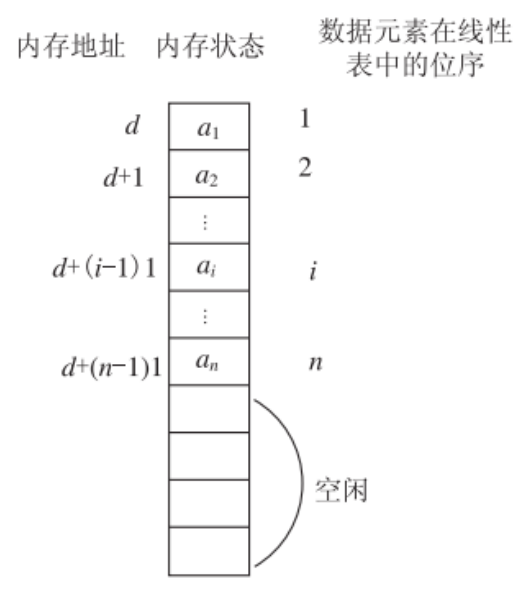
\includegraphics[width=0.6\textwidth]{assets/images/seqlist.png}
	\caption{线性表的逻辑结构示意图}
	\label{fig:seqlist} % 这里的标签名是用来引用的
	\cite{yan2012data}
\end{figure}

\subsection{系统设计}

\subsubsection{头文件和封装}

\paragraph{1. 头文件 }
此为代码用到的头文件，头文件为对数据结构的进一步封装，将在附录中给出。

\begin{lstlisting}
	#include <alib5/ds/vector.h>
	#include <alib5/aalgorithm.h>	
\end{lstlisting}

\paragraph{ 2.封装 } 此为代码对底层数据结构的一次封装用于实现ADT函数。

\begin{lstlisting}
	namespace hust_ds::sq_list{
		using namespace alib5::ds;
		/// 使用1-based的索引体系
		constexpr VectorTraits traits = [](){
			VectorTraits traits;
			// 1-based index support
			traits.offset = -1;
			return traits;
		}();
		/// 数据类型为int
		using Type = int;
		/// 使用std::allocator分配内存
		using Allocator = std::allocator<int>;
		/// 设置容器类型
		using Container = Vector<int,traits,Allocator>;
		/// 匹配头歌系统中的类型
		using List = Container*;
		/// 匹配头歌系统的Status设置
		enum class Status : int {
			Infeasible = -1,
			OK = 0,
			Error = 1,
		};
	}
\end{lstlisting}


\subsubsection{基本功能函数}

\begin{figure}[htbp]
	\centering
	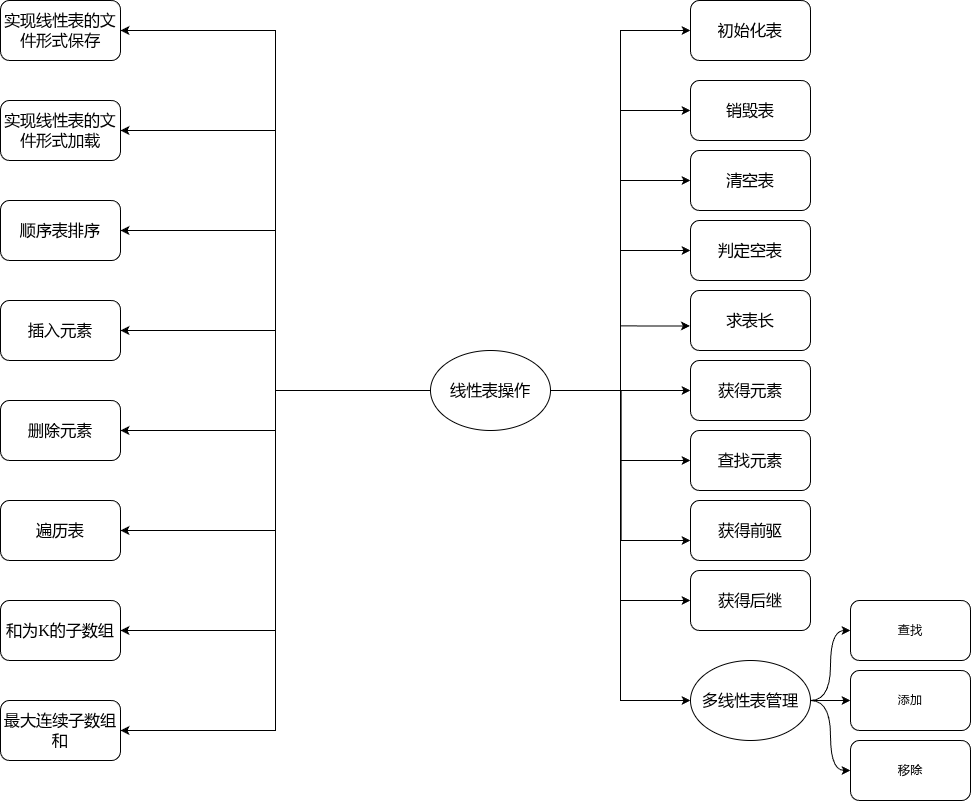
\includegraphics[width=1.0\textwidth]{assets/images/seqlist_needs.png}
	\caption{演示系统需要支持的功能}
	\label{fig:seqlist_structure} % 这里的标签名是用来引用的
\end{figure}


线性表的逻辑结构定义如下 \cite{yan2012data}：
\begin{equation*}
	\text{ADT List} \{
	\begin{aligned}
		&\text{数据对象：} D = \{a_i \mid a_i \in \text{ElemSet}, i = 1, 2, \dots, n, n \ge 0\} \\
		&\text{数据关系：} R_1 = \{\langle a_{i-1}, a_i \rangle \mid a_{i-1}, a_i \in D, i = 2, \dots, n\}
	\end{aligned}
	\}
\end{equation*}

遵循最小完备性与常用性相结合的原则，本实验实现了20种操作，具体功能如下：

\noindent
\begin{tabularx}{\textwidth}{p{4.5cm} X} % p{4.5cm}固定标签宽度，X自动适配剩余空间
	\textbf{InitList(L)} & 初始化表：构造一个空的线性表。 \\
	\textbf{DestroyList(L)} & 销毁表：销毁已存在的线性表 $L$。 \\
	\textbf{ClearList(L)} & 清空表：将线性表 $L$ 重置为空表。 \\
	\textbf{ListEmpty(L)} & 判定空表：若 $L$ 为空，返回 TRUE，否则返回 FALSE。 \\
	\textbf{ListLength(L)} & 求表长：返回 $L$ 中数据元素的个数。 \\
	\textbf{GetElem(L,i,e)} & 获得元素：用 $e$ 返回 $L$ 中第 $i$ 个数据元素的值。 \\
	\textbf{LocateElem(L,e,compare)} & 查找元素：返回表中首个与 $e$ 满足 \texttt{compare()} 关系的数据元素位序；不存在则返回 0。 \\
	\textbf{PriorElem(L,cur,pre)} & 获得前驱：若 \texttt{cur} 是 $L$ 的元素且非首元素，用 \texttt{pre} 返回其前驱。 \\
	\textbf{NextElem(L,cur,next)} & 获得后继：若 \texttt{cur} 是 $L$ 的元素且非末元素，用 \texttt{next} 返回其后继。 \\
	\textbf{ListInsert(L,i,e)} & 插入元素：在 $L$ 的第 $i$ 个位置前插入新元素 $e$。 \\
	\textbf{ListDelete(L,i,e)} & 删除元素：删除 $L$ 中第 $i$ 个数据元素，并用 $e$ 返回其值。 \\
	\textbf{ListTraverse(L,visit)} & 遍历表：依次对 $L$ 的每个元素调用 \texttt{visit()} 函数。 \\
	\textbf{MaxSubArray(L)} & 最大连续子数组和：计算并返回数组中和最大的连续子数组。 \\
	\textbf{SubArrayNum(L,k)} & 和为 K 的子数组：统计数组中所有和为 $k$ 的连续子数组个数。 \\
	\textbf{sortList(L)} & 顺序表排序：将线性表 $L$ 中的元素按升序排列。 \\
	\textbf{SaveList(L,FileName)} & 文件写入：将线性表 $L$ 的元素保存到指定文件中。 \\
	\textbf{LoadList(L,FileName)} & 文件读出：从指定文件读取数据并加载到线性表 $L$ 中。 \\
	\textbf{AddList/RemoveList} & 线性表管理：创建或移除集合中的特定线性表。 \\
	\textbf{LocateList/TraverseList} & 查找与遍历：查找指定线性表的索引或遍历所有线性表。 \\
	\textbf{SelectList(Lists, i)} & 选择表：将索引为 $i$ 的线性表设为当前操作对象。 \\
\end{tabularx}

\subsection{系统实现}

\subsubsection{演示系统框架}
本系统的交互框架主要封装在 \texttt{App} 类中，通过 \texttt{while(true)} 无限循环配合 \texttt{system("cls || clear")} 清屏命令，构建了一个跨平台、界面整洁的菜单驱动系统。
系统通过读取用户输入的命令字符串进行解析。为了支持多表操作，系统底层通过 \texttt{Vector<TableInstance> tables} 管理多个线性表实例，并利用 \texttt{active\_idx} 记录当前激活的线性表下标。用户可以通过 M1 至 M3 指令实现表的创建、切换和销毁；输入 1 至 17 的数字则通过 \texttt{switch-case} 语句路由至具体的底层数据结构算法模块。每次执行完毕后利用 \texttt{pause()} 函数暂停界面，提升了用户的交互体验。

\subsubsection{数据结构设计}
系统的底层数据结构未使用标准库容器，而是基于自行实现的模板类Vector，具有较好的定制性：

\textbf{1. 线性表（Vector 容器）}：通过泛型 \texttt{T} 和 \texttt{std::allocator} \cite{cppref} 实现内存分配。包含核心成员 \texttt{m\_data}（数据首地址指针）、\texttt{m\_length}（当前逻辑长度）和 \texttt{m\_capacity}（当前物理容量）。为了对齐课程教材的逻辑起点，引入了 \texttt{VectorTraits} 机制，配置 \texttt{offset = -1}，使得底层的 0-based 数组能够映射为上层的 1-based 逻辑位序。

\textbf{2. 实例管理表（TableInstance）}：封装了 \texttt{Vector<char> name}（用于存储字符串表名）以及 \texttt{List list}（即 \texttt{Vector<int>*} 指针），作为多表管理的最小单元。

\subsubsection{函数思想及实现}
说明：为保证系统的健壮性，本实现中所有基本操作函数在执行实质逻辑前，均会进行指针判空操作，若未初始化则直接拦截并返回 \texttt{Infeasible} 状态码。

\vspace{0.5em}
\noindent\textbf{1. 初始化线性表 (InitList)}
\newline\textbf{输入}：线性表指针的引用 (\texttt{List\&})
\newline\textbf{输出}：函数运行状态 (\texttt{Status})
\newline\textbf{函数思想描述}：判断传入的线性表指针是否为空。若非空说明已初始化，返回错误状态；若为空，则在堆区 \texttt{new} 一个 \texttt{Container} 对象，将首地址赋给引用指针。底层构造函数会自动初始化容量与长度。

\vspace{0.5em}
\noindent\textbf{2. 销毁线性表 (DestroyList)}
\newline\textbf{输入}：线性表指针的引用 (\texttt{List\&})
\newline\textbf{输出}：函数运行状态 (\texttt{Status})
\newline\textbf{函数思想描述}：检查指针有效性后，使用 \texttt{delete} 释放以该指针为首地址的堆内存区。为了防止悬垂指针问题，释放后立即将指针置为 \texttt{nullptr}。

\vspace{0.5em}
\noindent\textbf{3. 清空线性表 (ClearList)}
\newline\textbf{输入}：线性表指针的引用 (\texttt{List\&})
\newline\textbf{输出}：函数运行状态 (\texttt{Status})
\newline\textbf{函数思想描述}：调用底层 \texttt{Vector} 的 \texttt{clear()} 方法。该方法内部会判断数据类型是否为平凡析构类型，若非平凡则循环调用析构函数，最后将 \texttt{m\_length} 置为 0，而不释放物理容量（\texttt{m\_capacity} 保持不变），以便后续快速写入。

\vspace{0.5em}
\noindent\textbf{4. 判断线性表是否为空 (ListEmpty)}
\newline\textbf{输入}：线性表指针的引用 (\texttt{List\&})
\newline\textbf{输出}：\texttt{std::pair<bool, Status>}（包含布尔结果及运行状态）
\newline\textbf{函数思想描述}：首先检查表是否存在。若存在，则直接调用底层 \texttt{empty()} 接口判断 \texttt{m\_length} 是否为 0，通过 \texttt{C++17} 的结构化绑定特性返回包含结果和状态码的 \texttt{pair} 对。

\vspace{0.5em}
\noindent\textbf{5. 求线性表长度 (ListLength)}
\newline\textbf{输入}：线性表指针的引用 (\texttt{List\&})
\newline\textbf{输出}：整型变量（当前表中元素的数目）
\newline\textbf{函数思想描述}：校验有效性后，直接返回底层对象的 \texttt{length()} 方法结果，该操作的时间复杂度为 $O(1)$。

\vspace{0.5em}
\noindent\textbf{6. 访问元素 (GetElem)}
\newline\textbf{输入}：线性表引用 (\texttt{List\&})，整型位序 \texttt{i}，存储引用的变量 \texttt{e}
\newline\textbf{输出}：函数运行状态 (\texttt{Status})
\newline\textbf{函数思想描述}：判断传入的位序 \texttt{i} 的合法性。底层容器利用 \texttt{VectorTraits} 的 \texttt{offset} 属性，自动将逻辑索引 \texttt{i} 转换为物理索引 \texttt{i-1}。若不越界则通过引用参数 \texttt{e} 传出元素值，返回 \texttt{OK}。

\vspace{0.5em}
\noindent\textbf{7. 查找元素 (LocateElem)}
\newline\textbf{输入}：线性表引用 (\texttt{List\&})，待查元素 \texttt{e}，泛型比较器 \texttt{CompareFn\&\&}
\newline\textbf{输出}：整型变量（首个匹配元素的逻辑索引，失败返回 0）
\newline\textbf{函数思想描述}：采用泛型实现。通过将比较逻辑作为 \texttt{Lambda} 表达式传入底层的 \texttt{find()} 方法进行线性遍历。若查找到对应地址的指针 \texttt{ptr}，则利用指针相减（\texttt{ptr - begin()}）得出物理偏移，再通过减去 \texttt{traits.offset} 反算出以 1 为基准的逻辑索引。

\vspace{0.5em}
\noindent\textbf{8. 获取前驱元素 (PriorElem)}
\newline\textbf{输入}：线性表引用 (\texttt{List\&})，当前元素 \texttt{cur\_e}，存储引用的变量 \texttt{pre\_e}
\newline\textbf{输出}：函数运行状态 (\texttt{Status})
\newline\textbf{函数思想描述}：利用 \texttt{find()} 方法定位首个匹配项指针 \texttt{ptr}。若未找到或该指针等于 \texttt{begin()}（即首元素，无前驱），则返回错误；否则通过 \texttt{*(ptr - 1)} 获取前驱值赋予 \texttt{pre\_e}。

\vspace{0.5em}
\noindent\textbf{9. 获取后继元素 (NextElem)}
\newline\textbf{输入}：线性表引用 (\texttt{List\&})，当前元素 \texttt{cur\_e}，存储引用的变量 \texttt{next\_e}
\newline\textbf{输出}：函数运行状态 (\texttt{Status})
\newline\textbf{函数思想描述}：与获取前驱类似。找到目标指针 \texttt{ptr} 后，判断其是否为容器的 \texttt{end()} 或 \texttt{end()-1}（即尾元素，无后继）。合法时，通过 \texttt{*(ptr + 1)} 获取后继并返回 \texttt{OK}。

\vspace{0.5em}
\noindent\textbf{10. 插入元素 (ListInsert)}
\newline\textbf{输入}：线性表引用 (\texttt{List\&})，插入位序 \texttt{i}，待插入元素 \texttt{e}
\newline\textbf{输出}：函数运行状态 (\texttt{Status})
\newline\textbf{函数思想描述}：调用底层容器的 \texttt{insert()}。若当前 \texttt{m\_length + 1 > m\_capacity}，系统触发两倍动态扩容，分配新空间并完成元素拷贝迁移。插入时，从尾部开始将 \texttt{i} 之后的元素逐个后移一个单元，腾出空间后写入新元素 \texttt{e}。

\vspace{0.5em}
\noindent\textbf{11. 删除元素 (ListDelete)}
\newline\textbf{输入}：线性表引用 (\texttt{List\&})，删除位序 \texttt{i}，存储变量引用 \texttt{e}
\newline\textbf{输出}：函数运行状态 (\texttt{Status})
\newline\textbf{函数思想描述}：首先进行上下界校验 ($1 \le i \le \mathrm{length}$)。调用底层 \texttt{remove()} 方法，将待删除元素通过移动语义转存至 \texttt{e} 中。随后将其后的元素依次前移覆盖目标内存，逻辑长度自减，返回 \texttt{OK}。

\vspace{0.5em}
\noindent\textbf{12. 遍历线性表 (ListTraverse)}
\newline\textbf{输入}：线性表引用 (\texttt{List\&})，泛型函数对象 \texttt{VisitFn\&\&}
\newline\textbf{输出}：函数运行状态 (\texttt{Status})
\newline\textbf{函数思想描述}：将遍历操作和业务逻辑（如打印）解耦。利用 C++11 的 \texttt{for-each} 语法迭代线性表，对每个元素执行传入的 \texttt{visit} 回调函数。

\vspace{0.5em}
\noindent\textbf{13. 求最大连续子数组和 (MaxSubArray) [附加功能]}
\newline\textbf{输入}：线性表引用 (\texttt{List\&})
\newline\textbf{输出}：整型变量（最大和）
\newline\textbf{算法描述}：采用动态规划的思想 \cite{cormen2009introduction}。初始化全局最大值 \texttt{max\_val} 和当前累计和 \texttt{curr\_max}。遍历线性表，通过状态转移方程 $\mathrm{curr\_max} = \max(\mathrm{list}[i], \mathrm{curr\_max} + \mathrm{list}[i])$ 不断舍弃产生负收益的前缀段，实时更新全局最值。
\newline\textbf{算法复杂度}：相比暴力的 $O(n^2)$，该算法仅需一次遍历，时间复杂度为 $O(n)$，空间复杂度为 $O(1)$。

\vspace{0.5em}
\noindent\textbf{14. 求特定和的连续子数组数目 (SubArrayNum) [附加功能]}
\newline\textbf{输入}：线性表引用 (\texttt{List\&})，目标和 \texttt{k}
\newline\textbf{输出}：整型变量（符合条件的子数组数目）
\newline\textbf{算法描述}：采用空间换时间的策略。复用底层的 \texttt{Container} 动态构建长度为 \texttt{len+1} 的前缀和数组 $P$。原数组区间 $[i, j]$ 的和可直接利用差分思想表示为 $P[j+1] - P[i]$。通过双重循环枚举前缀和差值，寻找等于目标 $k$ 的区间。
\newline\textbf{算法复杂度}：时间复杂度为 $O(n^2)$，空间复杂度为 $O(n)$。

\vspace{0.5em}
\noindent\textbf{15. 线性表排序 (SortList) [附加功能]}
\newline\textbf{输入}：线性表引用 (\texttt{List\&})
\newline\textbf{输出}：函数运行状态 (\texttt{Status})
\newline\textbf{算法描述}：基于自实现算法库引入了 \textbf{希尔排序 (Shell Sort)}。相比直接调用标准库的快速排序，希尔排序无需依赖栈或系统递归调用，避免了自实现底层结构时无法依赖标准库递归排序的循环依赖问题。
为了进一步优化性能，本系统采用了数学上经过优化的 \textbf{Knuth 增量序列}。同时，在底层实现中结合了 C++11 的 \texttt{std::move} \cite{cppref} 移动语义与泛型迭代器，避免了元素交换时的冗余深拷贝。其核心算法结构如下（包含模板元编程的完整源码详见附录）\cite{cormen2009introduction}：

\begin{lstlisting}
	// 1. 根据区间长度计算 Knuth 增量初始值 (h = 3*h + 1)
	size_t gap = 1;
	while (gap < len / 3) {
		gap = 3 * gap + 1; 
	}
	
	// 2. 核心排序逻辑（基于分组的带有间隙的插入排序）
	while (gap > 0) {
		// 遍历每一个增量分组
		for (size_t begin_pos = 0; begin_pos < gap; ++begin_pos) {
			// 在组内执行插入排序
			for (size_t c_begin = begin_pos + gap; c_begin < len; c_begin += gap) {
				IterType j = begin + c_begin;
				// 利用移动语义提取当前元素，避免拷贝
				value_t val = std::move(*j); 
				
				// 依据自定义 compare 比较并寻找插入位置，跨度为 gap
				while (j > (begin + begin_pos) && compare(val, *(j - gap))) {
					*j = std::move(*(j - gap)); // 元素按 gap 跨度后移
					j -= gap;
				}
				*j = std::move(val); // 元素填入最终的目标位置
			}
		}
		gap = gap / 3; // 缩小增量，进入下一轮
	}
\end{lstlisting}

\noindent\textbf{算法复杂度}：采用 Knuth 序列后，在百万级数据量下的时间复杂度稳定在 $O(n^{1.11})$ 左右（与普通快排的 $O(n\log n)$ 相当，且不存在最坏退化情况），结合 \texttt{std::move} 优化，空间复杂度仅为 $O(1)$。

\vspace{0.5em}
\noindent\textbf{16. 保存线性表 (SaveList) [附加功能]}
\newline\textbf{输入}：线性表引用 (\texttt{List\&})，文件路径字符串
\newline\textbf{输出}：函数运行状态 (\texttt{Status})
\newline\textbf{函数思想描述}：以二进制只写模式（\texttt{"wb"}）打开文件。在文件头写入 \texttt{"SEQL"} 魔数（Magic Number）用于格式识别，随后利用 \texttt{fwrite} 依次写入元素个数 (\texttt{length})、每个元素的字节大小 (\texttt{sizeof(Type)}) 以及内存块数据。

\vspace{0.5em}
\noindent\textbf{17. 加载线性表 (LoadList) [附加功能]}
\newline\textbf{输入}：线性表引用 (\texttt{List\&})，文件路径字符串
\newline\textbf{输出}：函数运行状态 (\texttt{Status})
\newline\textbf{函数思想描述}：以二进制只读模式打开文件。首先读取前 4 字节并用 \texttt{memcmp} 与魔数 \texttt{"SEQL"} 比较，若不匹配则停止读取以防出错。随后校验 \texttt{sizeof(Type)}，数据对齐无误后清理当前表内容，重新分配内存并通过 \texttt{fread} 一次性将文件数据读入内存。

\vspace{0.5em}
\noindent\textbf{18. 多表管理操作 (create\_table / switch\_table / remove\_table)}
\newline\textbf{输入}：用户输入指令及内部映射表
\newline\textbf{输出}：对应管理状态的变化
\newline\textbf{函数思想描述}：作为整个系统的管理模块，\texttt{create\_table} 创建 \texttt{TableInstance} 实例并加入管理容器（采用 \texttt{std::move} 避免深拷贝）；\texttt{switch\_table} 通过修改 \texttt{active\_idx} 来切换当前操作的表；\texttt{remove\_table} 在移除前调用 \texttt{DestroyList} 避免内存泄漏，并从管理容器中删除对应实例。

\subsection{系统测试}

\subsubsection{测试环境与总体测试集设计}
系统的核心演示框架主菜单界面如图 \ref{fig:menu} 所示。为了验证顺序表 ADT 各项基本功能及附加算法的正确性、健壮性和鲁棒性，本实验设计了 4 个维度的测试集进行交叉覆盖测试：

\begin{itemize}
	\item \textbf{测试集 1（基础功能与文件存取）}：重点验证单表状态下的增删改查、属性获取以及二进制文件保存与读取功能。目标数据序列：\texttt{1 3 5 7 9}。
	\item \textbf{测试集 2（附加算法）}：通过包含正负交替数据的序列，重点验证最大连续子数组和、目标和子串计数及希尔排序功能。目标数据序列：\texttt{-2 1 -3 4 -1 2 1 -5 4}。
	\item \textbf{测试集 3（边界与异常处理）}：验证系统对未初始化访问、重复构建/销毁、越界读写以及空节点前后继查询的非法操作拦截能力。
	\item \textbf{测试集 4（多表管理）}：验证多实例管理下，数据表的创建、切换、各表数据互不影响以及销毁时的动态调整机制。
\end{itemize}

\begin{figure}[htbp]
	\centering
	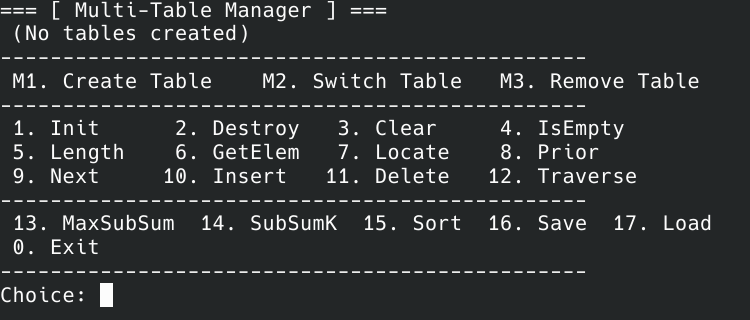
\includegraphics[width=0.6\textwidth]{assets/images/sq_test/menu.png}
	\caption{演示系统主菜单界面}
	\label{fig:menu}
\end{figure}

\subsubsection{测试集 1：基本功能与文件操作测试}
\begin{table}[htbp]
	\centering
	\caption{测试集 1 核心功能测试用例明细}
	\vspace{0.5em}
	% 借助 array 宏包，使用 >{\centering\arraybackslash} 让 p 列文字居中
	\begin{tabular}{|>{\centering\arraybackslash}p{3cm}|>{\centering\arraybackslash}p{3.5cm}|>{\centering\arraybackslash}p{4.5cm}|c|}
		\hline
		\textbf{测试项} & \textbf{测试输入动作} & \textbf{预期结果} & \textbf{实际结果} \\ \hline
		建表与初始化 & 创建 TestList1，输入 1 & 提示创建成功，初始化返回 OK(0) & 一致 \\ \hline
		连续插入元素 & 依次插入 1, 3, 5, 7, 9 & 遍历输出 \texttt{1 3 5 7 9} & 一致 \\ \hline
		求长与判空 & 输入 5，输入 4 & 长度为 5，IsEmpty 为 FALSE & 一致 \\ \hline
		随机访问与查找 & 获取位序 3，查找 5 & 返回元素 5，返回首个位序 3 & 一致 \\ \hline
		前驱与后继 & 求 5 的前驱，5 的后继 & 5 的前驱为 3，后继为 7 & 一致 \\ \hline
		删除操作 & 删除位序 2 的元素 & 遍历输出变为 \texttt{1 5 7 9} & 一致 \\ \hline
		文件保存与清空 & 保存到 test1.bin，执行 Clear & 文件生成，遍历为空表 & 一致 \\ \hline
		文件读取与恢复 & 从 test1.bin 读取数据 & 遍历输出恢复为 \texttt{1 5 7 9} & 一致 \\ \hline
		内存销毁 & 执行 Destroy (2) & 返回 OK(0)，内存正确释放 & 一致 \\ \hline
	\end{tabular}
	\label{tab:test_suite_1}
\end{table}

\textbf{测试过程与截图验证：}

首先创建多表管理单元并完成底层内存初始化，随后依次插入测试集数据并进行遍历。
\begin{figure}[htbp]
	\centering
	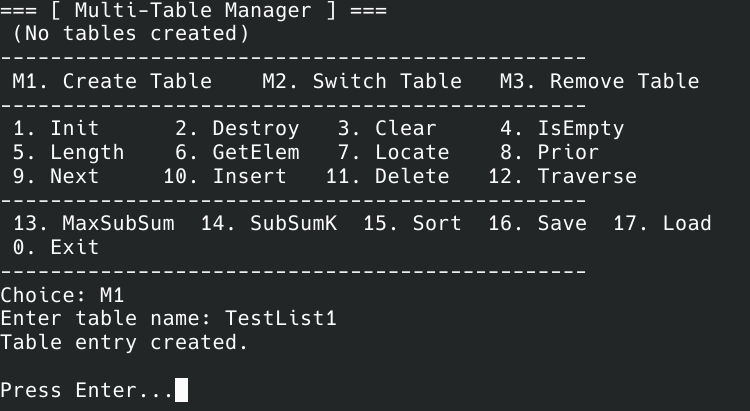
\includegraphics[width=0.6\textwidth]{assets/images/sq_test/create_list.png}
	\caption{创建测试表实例 TestList1}
	\label{fig:ts1_create}
\end{figure}
\begin{figure}[htbp]
	\centering
	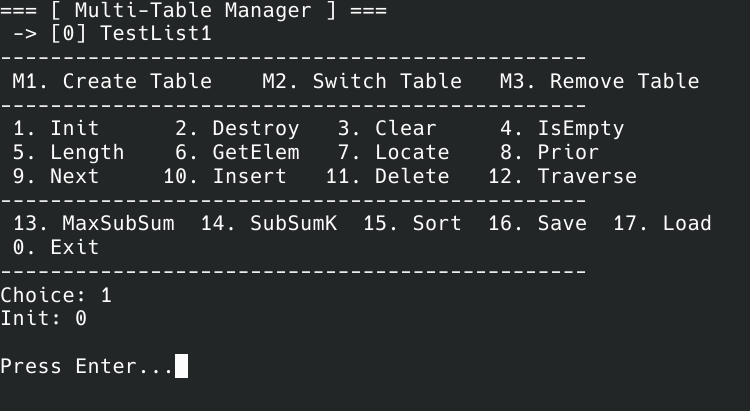
\includegraphics[width=0.6\textwidth]{assets/images/sq_test/init_list.png}
	\caption{底层顺序表 InitList 初始化分配}
	\label{fig:ts1_init}
\end{figure}
\begin{figure}[htbp]
	\centering
	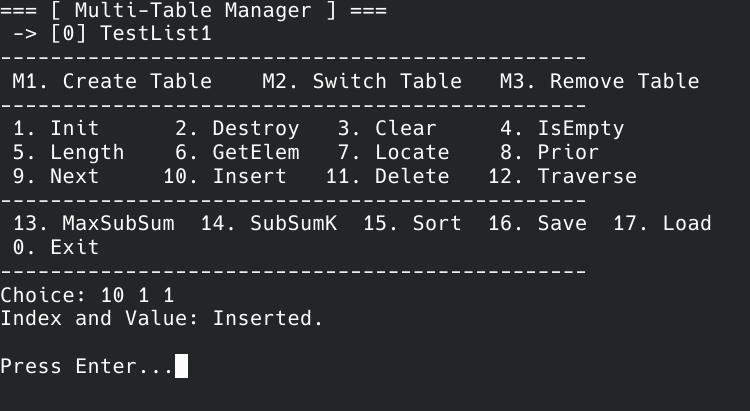
\includegraphics[width=0.6\textwidth]{assets/images/sq_test/insert_data.png}
	\caption{依次插入测试数据}
	\label{fig:ts1_insert}
\end{figure}
\begin{figure}[htbp]
	\centering
	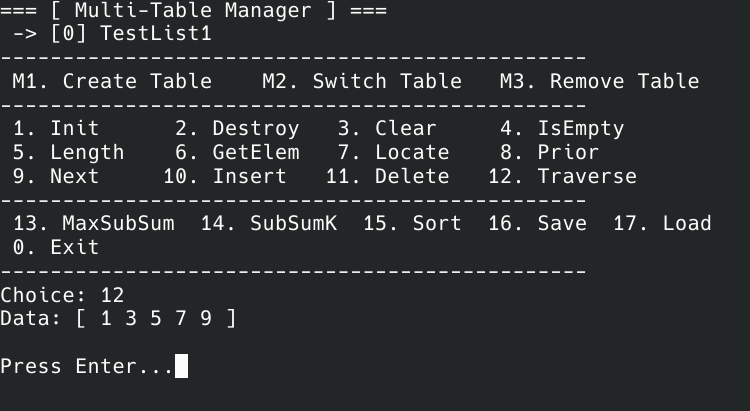
\includegraphics[width=0.6\textwidth]{assets/images/sq_test/foreach_1.png}
	\caption{插入数据后 Traverse 遍历结果}
	\label{fig:ts1_foreach1}
\end{figure}

针对当前数据集合，进行属性查询与元素检索：
\begin{figure}[htbp]
	\centering
	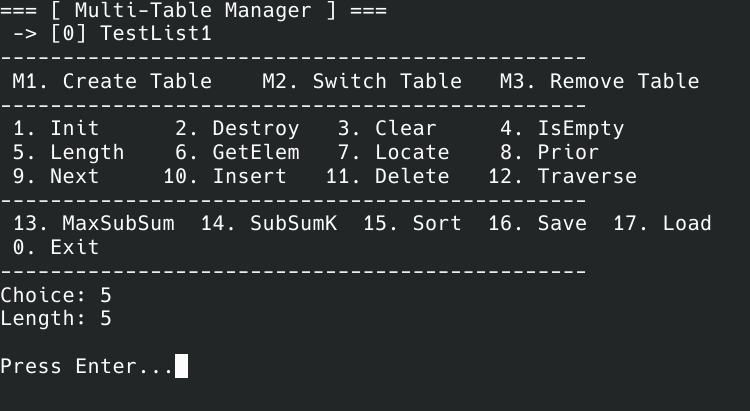
\includegraphics[width=0.6\textwidth]{assets/images/sq_test/len.png}
	\caption{测试求取当前表长}
	\label{fig:ts1_len}
\end{figure}
\begin{figure}[htbp]
	\centering
	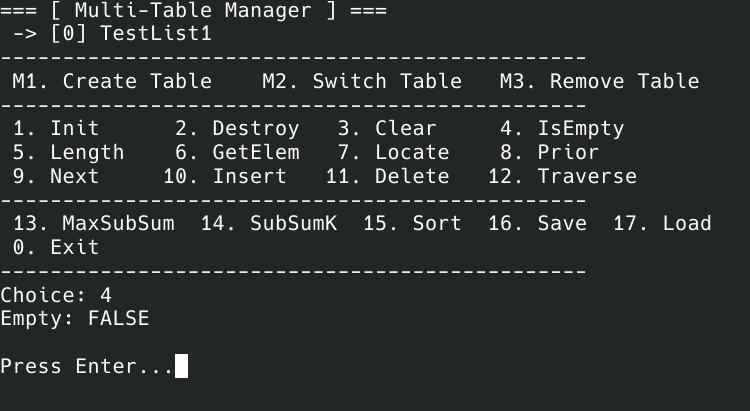
\includegraphics[width=0.6\textwidth]{assets/images/sq_test/empty.png}
	\caption{测试空表逻辑判断}
	\label{fig:ts1_empty}
\end{figure}
\begin{figure}[htbp]
	\centering
	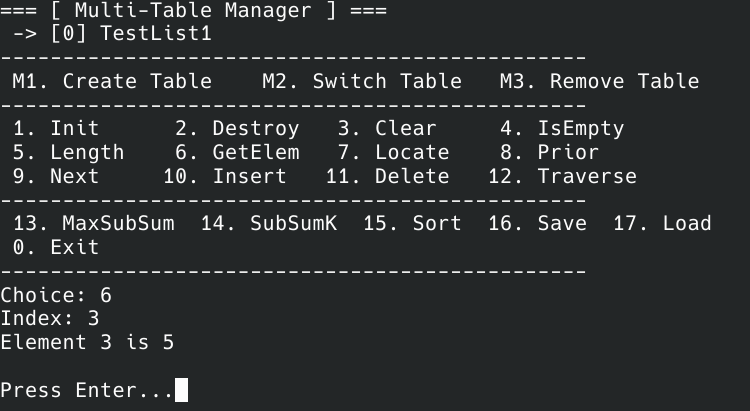
\includegraphics[width=0.6\textwidth]{assets/images/sq_test/3_rd.png}
	\caption{通过 GetElem 获取逻辑索引为 3 的元素}
	\label{fig:ts1_3rd}
\end{figure}
\begin{figure}[htbp]
	\centering
	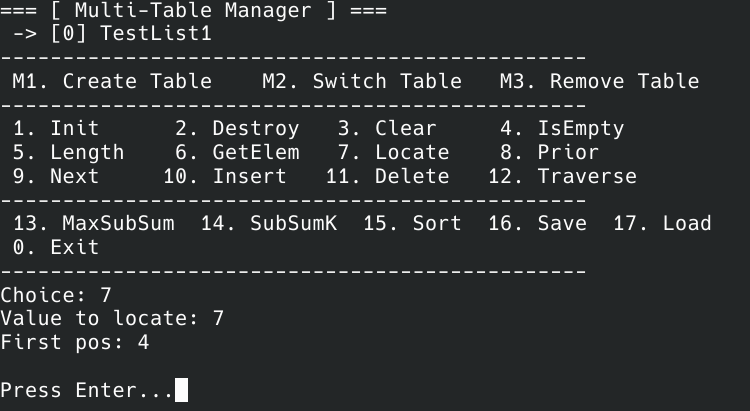
\includegraphics[width=0.6\textwidth]{assets/images/sq_test/locate.png}
	\caption{通过 Locate 检索元素位序}
	\label{fig:ts1_locate}
\end{figure}
\begin{figure}[htbp]
	\centering
	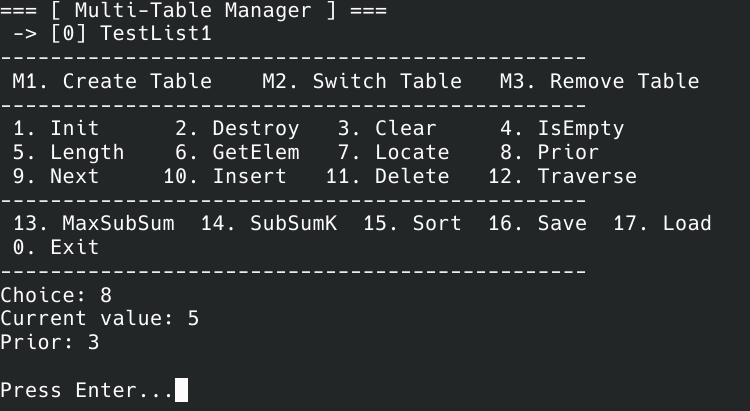
\includegraphics[width=0.6\textwidth]{assets/images/sq_test/prior.png}
	\caption{获取目标元素的前驱}
	\label{fig:ts1_prior}
\end{figure}
\begin{figure}[htbp]
	\centering
	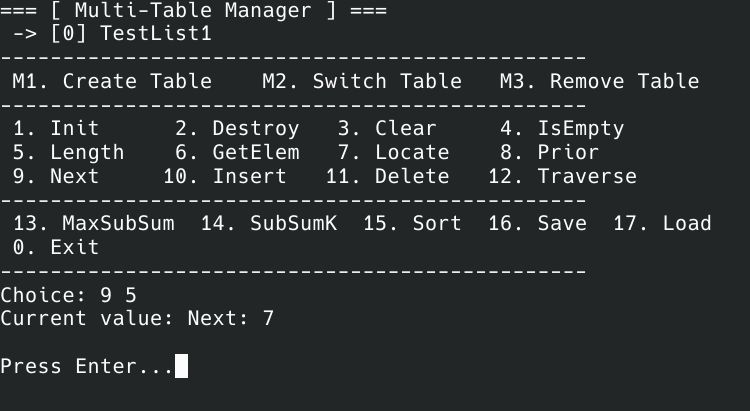
\includegraphics[width=0.6\textwidth]{assets/images/sq_test/next.png}
	\caption{获取目标元素的后继}
	\label{fig:ts1_next}
\end{figure}

为验证逻辑结构的动态维护能力，进行定点删除操作，并在确认数据更新后测试二进制文件存取能力。
\begin{figure}[htbp]
	\centering
	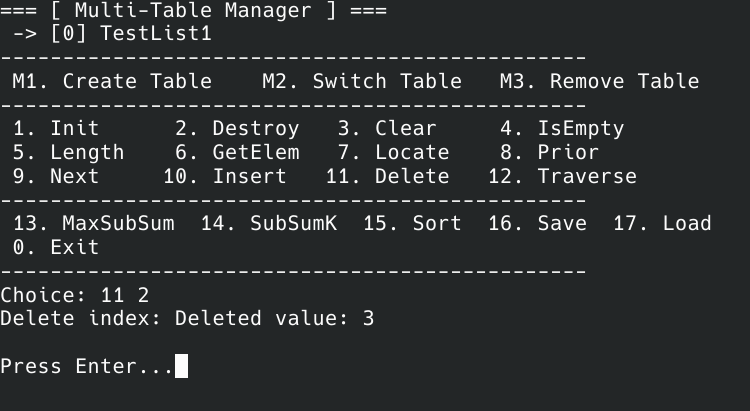
\includegraphics[width=0.6\textwidth]{assets/images/sq_test/delete.png}
	\caption{执行 ListDelete 删除特定位置元素}
	\label{fig:ts1_delete}
\end{figure}
\begin{figure}[htbp]
	\centering
	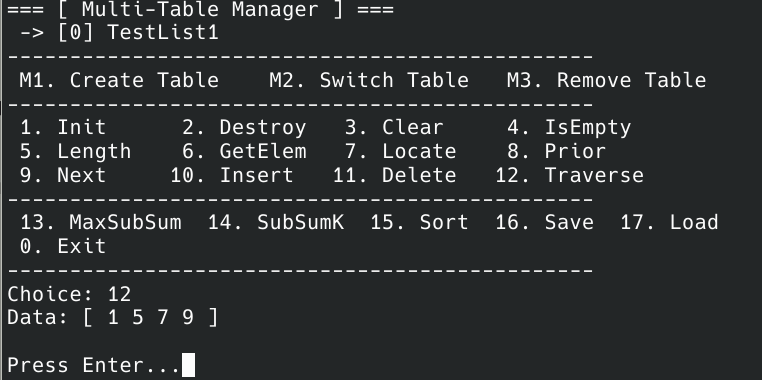
\includegraphics[width=0.6\textwidth]{assets/images/sq_test/foreach_2.png}
	\caption{删除操作后的 Traverse 验证}
	\label{fig:ts1_foreach2}
\end{figure}
\begin{figure}[htbp]
	\centering
	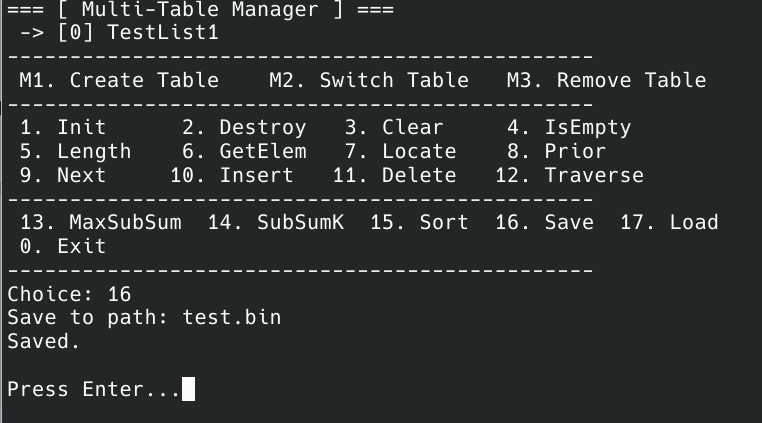
\includegraphics[width=0.6\textwidth]{assets/images/sq_test/save.png}
	\caption{将当前内存数据保存为 bin 格式文件}
	\label{fig:ts1_save}
\end{figure}
\begin{figure}[htbp]
	\centering
	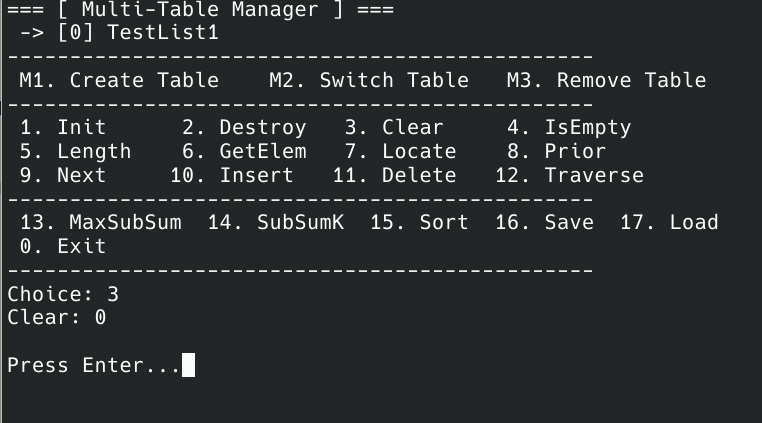
\includegraphics[width=0.6\textwidth]{assets/images/sq_test/clear.png}
	\caption{利用 Clear 功能清空表内元素}
	\label{fig:ts1_clear}
\end{figure}
\begin{figure}[htbp]
	\centering
	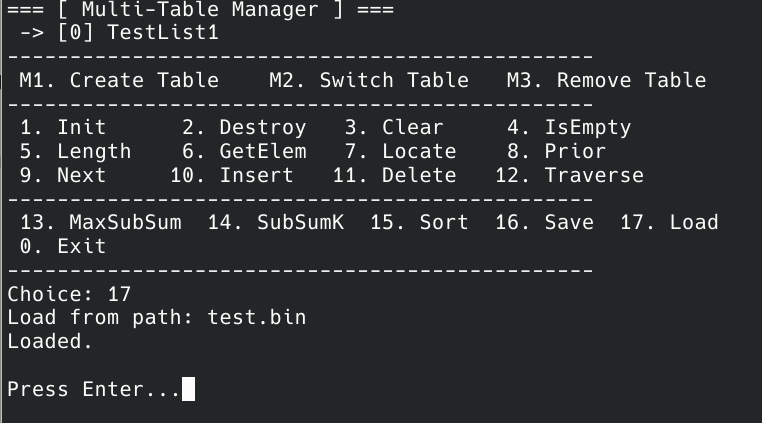
\includegraphics[width=0.6\textwidth]{assets/images/sq_test/load.png}
	\caption{从 bin 格式文件中读取并加载数据}
	\label{fig:ts1_load}
\end{figure}
\begin{figure}[htbp]
	\centering
	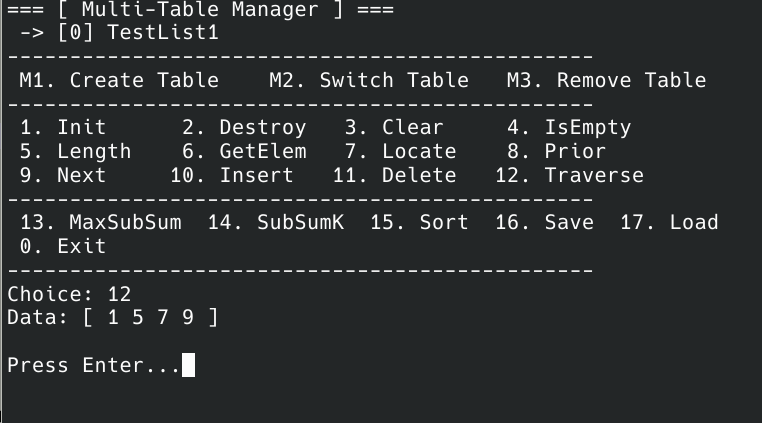
\includegraphics[width=0.6\textwidth]{assets/images/sq_test/foreach_3.png}
	\caption{Load 操作完成后遍历确认数据完整恢复}
	\label{fig:ts1_foreach3}
\end{figure}
\begin{figure}[htbp]
	\centering
	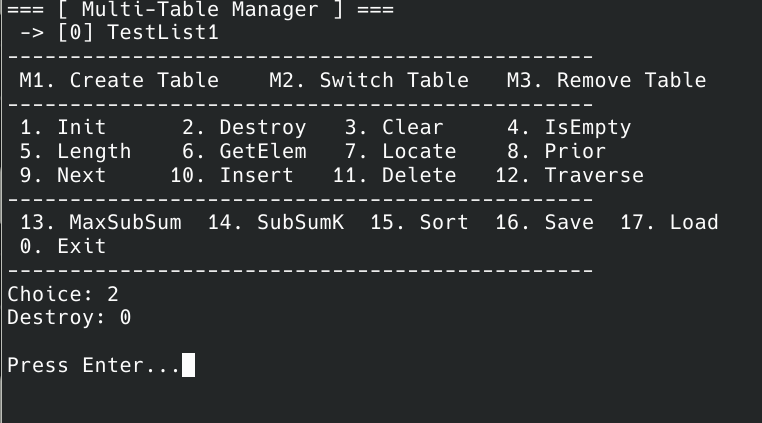
\includegraphics[width=0.6\textwidth]{assets/images/sq_test/destroy.png}
	\caption{执行 Destroy 销毁表并释放堆内存}
	\label{fig:ts1_destroy}
\end{figure}

\subsubsection{测试集 2：算法与附加功能测试}

本部分重点测试自实现顺序表上运行附加算法的表现。构建包含正负数的集合：\texttt{-2 1 -3 4 -1 2 1 -5 4}。
\begin{figure}[htbp]
	\centering
	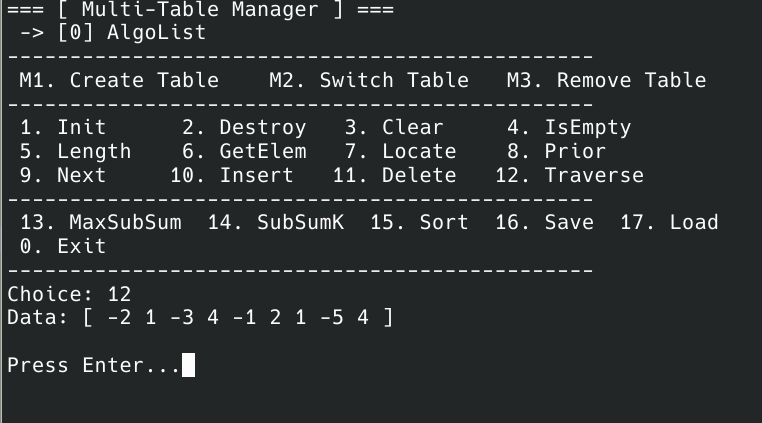
\includegraphics[width=0.6\textwidth]{assets/images/sq_test/algoready.png}
	\caption{算法测试集基础数据构建完毕}
	\label{fig:ts2_ready}
\end{figure}

\textbf{算法点 1：求解最大连续子数组和 (MaxSubArray)}
系统采用了 $O(n)$ 复杂度的动态规划实现，对于当前集合，最大和的子段为 \texttt{[4, -1, 2, 1]}，预期和为 6。实际输出结果与理论一致：
\begin{figure}[htbp]
	\centering
	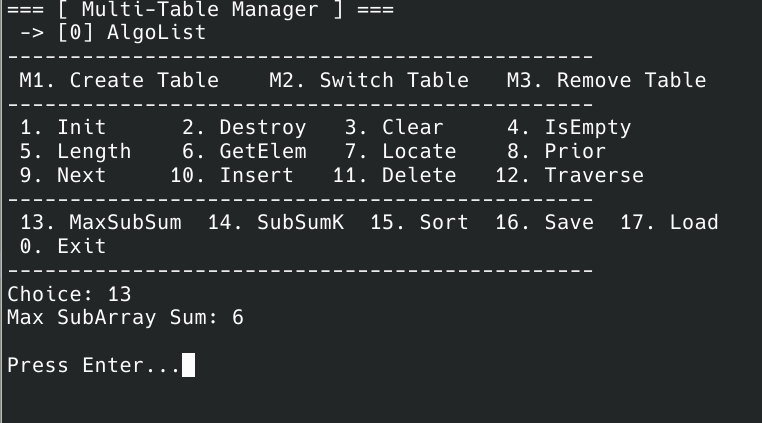
\includegraphics[width=0.6\textwidth]{assets/images/sq_test/max_sum.png}
	\caption{最大连续子数组和求解结果}
	\label{fig:ts2_maxsum}
\end{figure}

\textbf{算法点 2：统计和为 $K$ 的连续子数组数目 (SubArrayNum)}
测试令目标和 $K=3$。系统通过前缀和预处理算法计算得出匹配次数为 5。这 5 组满足条件的区间在逻辑上拆解如下（与实际验证完全符合）：

\begin{itemize}
	\item 下标 3 $\sim$ 4：\texttt{[4, -1]}，求和：$4 + (-1) = 3$
	\item 下标 5 $\sim$ 6：\texttt{[2, 1]}，求和：$2 + 1 = 3$
	\item 下标 1 $\sim$ 5：\texttt{[1, -3, 4, -1, 2]}，求和：$1 + (-3) + 4 + (-1) + 2 = 3$
	\item 下标 2 $\sim$ 6：\texttt{[-3, 4, -1, 2, 1]}，求和：$(-3) + 4 + (-1) + 2 + 1 = 3$
	\item 下标 1 $\sim$ 8：\texttt{[1, -3, 4, -1, 2, 1, -5, 4]}，求和：$1 + (-3) + 4 + (-1) + 2 + 1 + (-5) + 4 = 3$
\end{itemize}

\begin{figure}[htbp]
	\centering
	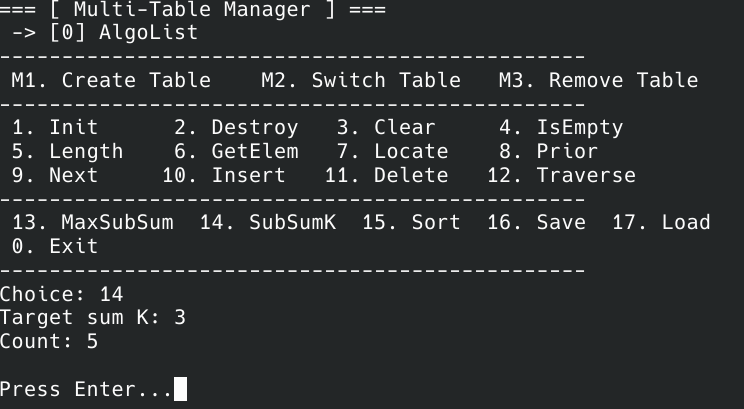
\includegraphics[width=0.6\textwidth]{assets/images/sq_test/sumk.png}
	\caption{特定和子数组数目统计结果}
	\label{fig:ts2_sumk}
\end{figure}

\textbf{算法点 3：底层希尔排序 (SortList)}
调用内置算法模块的 Knuth 序列希尔排序对集合进行递增重组，排序结果稳定且准确：
\begin{figure}[htbp]
	\centering
	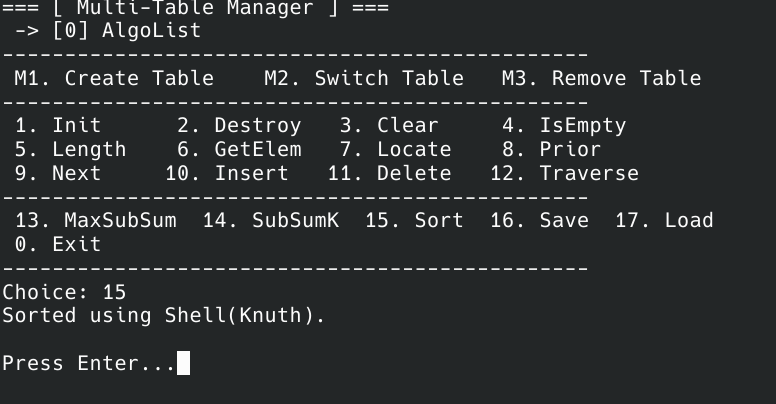
\includegraphics[width=0.6\textwidth]{assets/images/sq_test/sort.png}
	\caption{触发 Shell Sort 排序}
	\label{fig:ts2_sort}
\end{figure}
\begin{figure}[htbp]
	\centering
	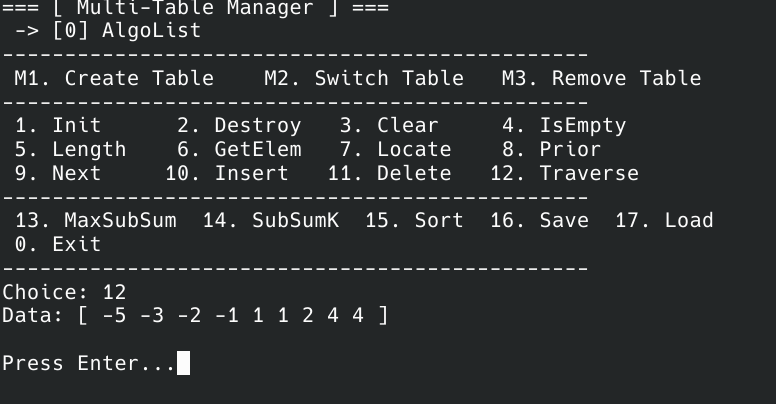
\includegraphics[width=0.6\textwidth]{assets/images/sq_test/after_sort.png}
	\caption{排序后的线性表有序形态}
	\label{fig:ts2_aftersort}
\end{figure}

\subsubsection{测试集 3：异常处理与边界测试}

健壮的系统需要能正确处理各种越界、空操作及非法调用。本节测试集中展示了系统底层异常捕获机制 \texttt{\_panic\_bounds} 与上层枚举状态码 \texttt{Infeasible / Error} 的协同拦截效果。

\begin{figure}[htbp]
	\centering
	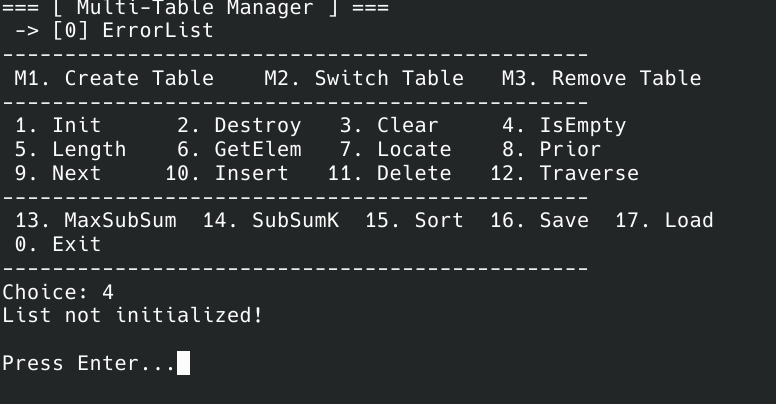
\includegraphics[width=0.6\textwidth]{assets/images/sq_test/not_init.png}
	\caption{测试：未初始化时拒绝执行读写功能}
	\label{fig:ts3_notinit}
\end{figure}
\begin{figure}[htbp]
	\centering
	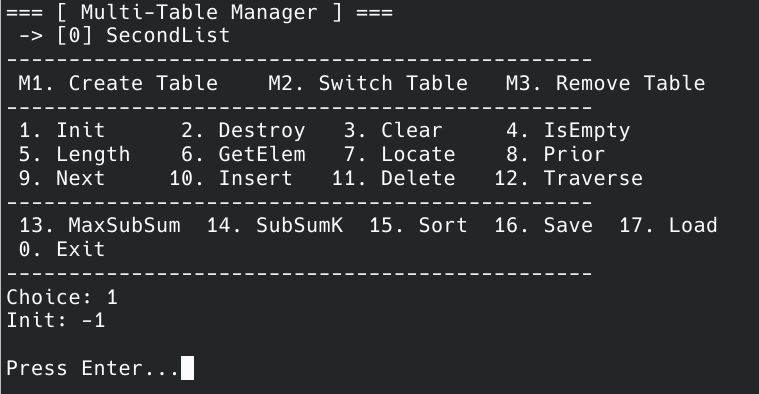
\includegraphics[width=0.6\textwidth]{assets/images/sq_test/reinit.png}
	\caption{测试：防止内存泄漏的重复 Init 拦截}
	\label{fig:ts3_reinit}
\end{figure}
\begin{figure}[htbp]
	\centering
	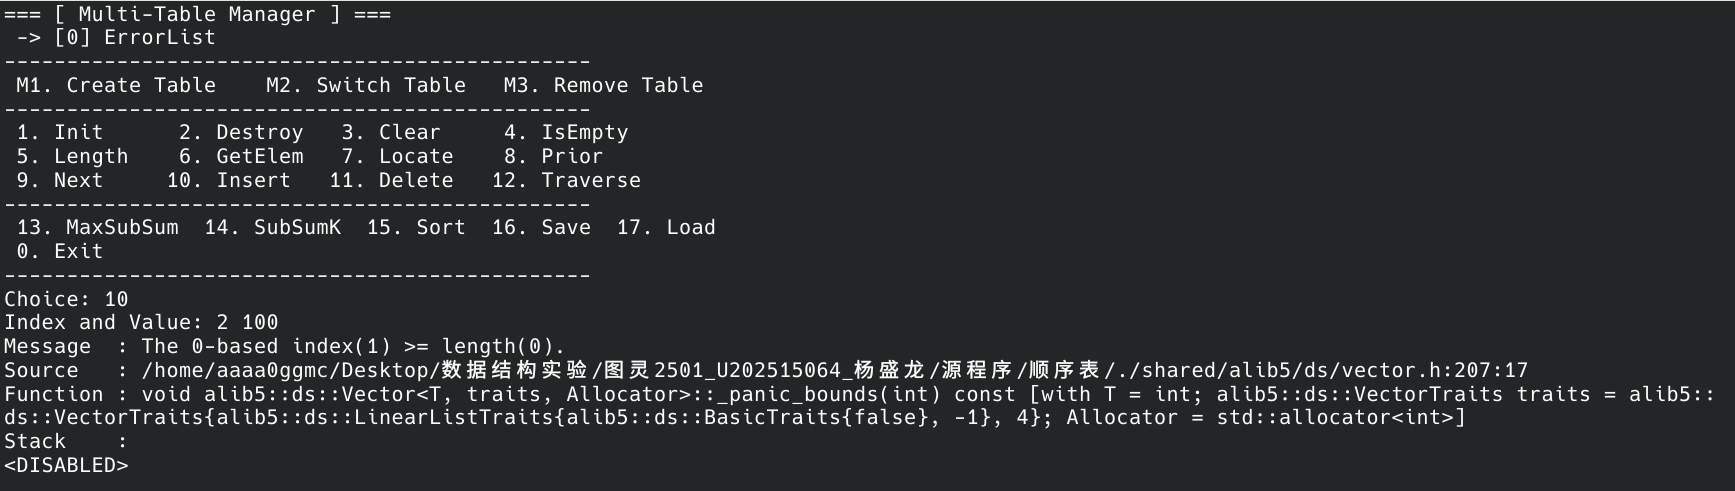
\includegraphics[width=0.6\textwidth]{assets/images/sq_test/alert_of_insert.png}
	\caption{测试：越界插入的错误提示}
	\label{fig:ts3_alert_insert}
\end{figure}

对于查找与前后继检索中的异常情况，系统也进行了相应捕获：
\begin{figure}[htbp]
	\centering
	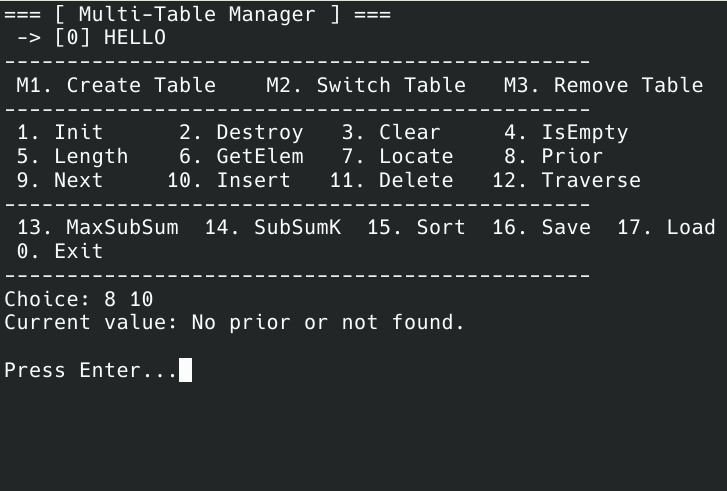
\includegraphics[width=0.6\textwidth]{assets/images/sq_test/no_prior.png}
	\caption{测试：首元素前驱越界访问拦截}
	\label{fig:ts3_no_prior}
\end{figure}
\begin{figure}[htbp]
	\centering
	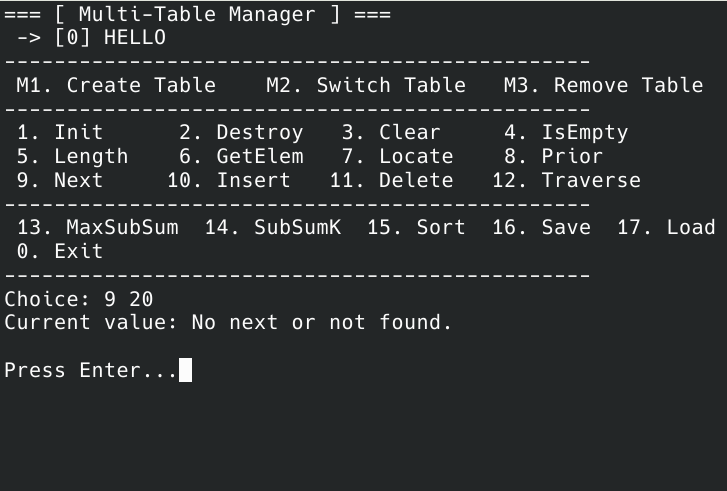
\includegraphics[width=0.6\textwidth]{assets/images/sq_test/no_next.png}
	\caption{测试：尾元素后继越界访问拦截}
	\label{fig:ts3_no_next}
\end{figure}
\begin{figure}[htbp]
	\centering
	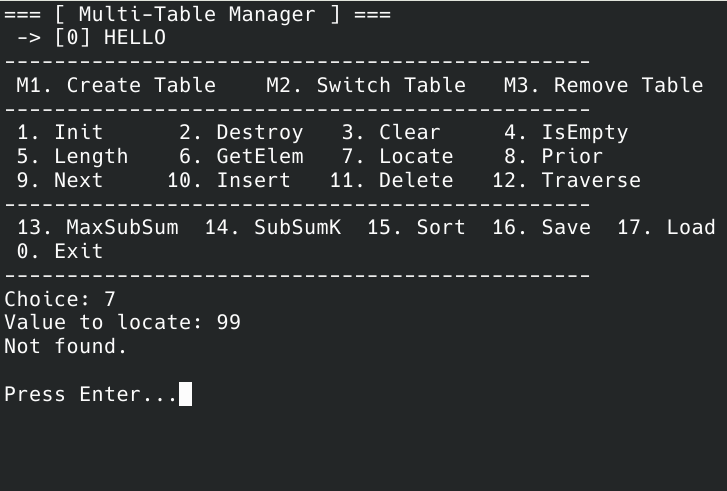
\includegraphics[width=0.6\textwidth]{assets/images/sq_test/nfound.png}
	\caption{测试：对不存在元素的查找匹配拦截}
	\label{fig:ts3_nfound}
\end{figure}
\begin{figure}[htbp]
	\centering
	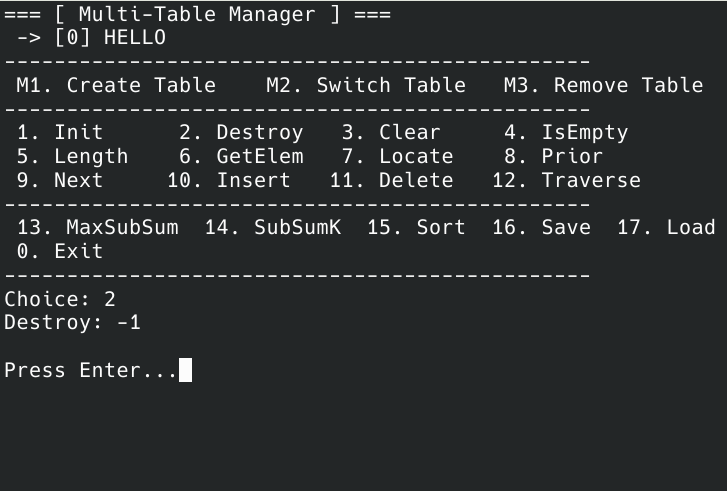
\includegraphics[width=0.6\textwidth]{assets/images/sq_test/redestr.png}
	\caption{测试：针对已销毁或未初始化的表重复执行 Destroy，系统拒绝并返回 -1}
	\label{fig:ts3_redestr}
\end{figure}

\subsubsection{测试集 4：多表管理与数据独立性测试}

首先创建基础表 1（L1），并确认其独立状态：
\begin{figure}[htbp]
	\centering
	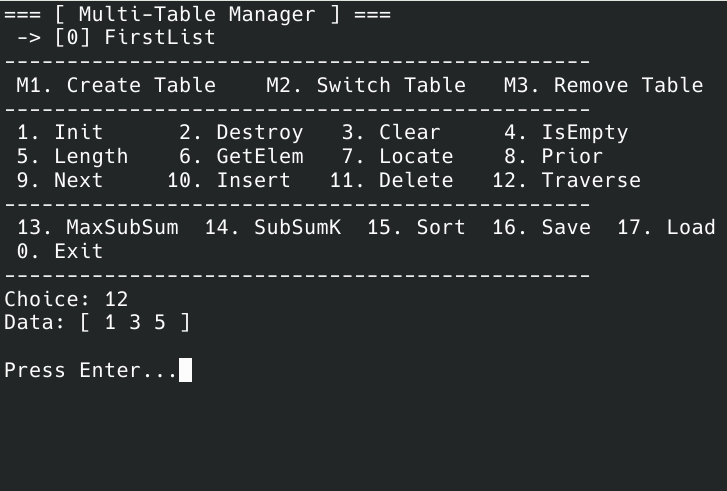
\includegraphics[width=0.6\textwidth]{assets/images/sq_test/l1.png}
	\caption{新建表 FirstList 的遍历状态}
	\label{fig:ts4_l1}
\end{figure}

随后新建表 2（SecondList）并切换至该表，可见两表数据互不影响：
\begin{figure}[htbp]
	\centering
	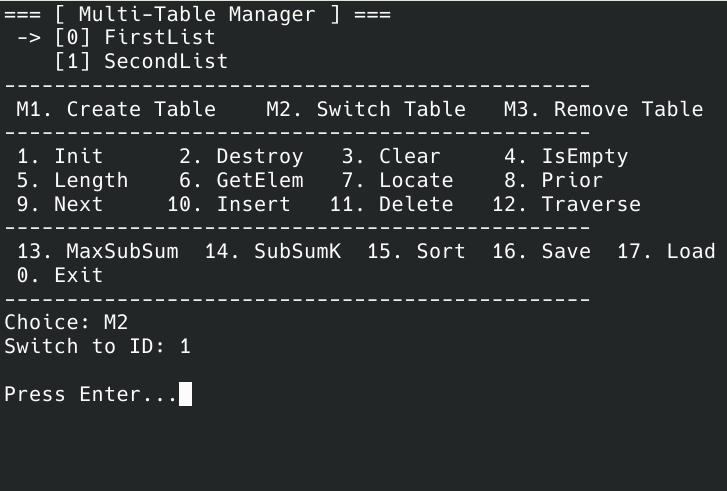
\includegraphics[width=0.6\textwidth]{assets/images/sq_test/switching.png}
	\caption{执行 Switch Table (M2) 切换至目标索引}
	\label{fig:ts4_switching}
\end{figure}
\begin{figure}[htbp]
	\centering
	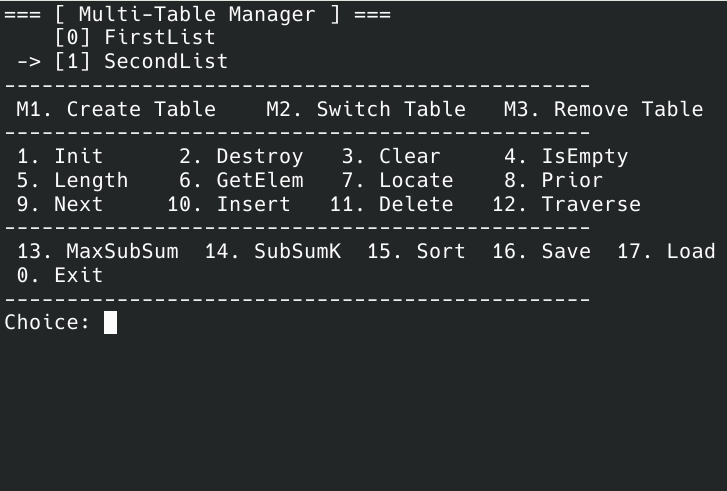
\includegraphics[width=0.6\textwidth]{assets/images/sq_test/switched.png}
	\caption{主菜单 UI 更新，当前激活标识 \texttt{->} 指向 SecondList}
	\label{fig:ts4_switched}
\end{figure}
\begin{figure}[htbp]
	\centering
	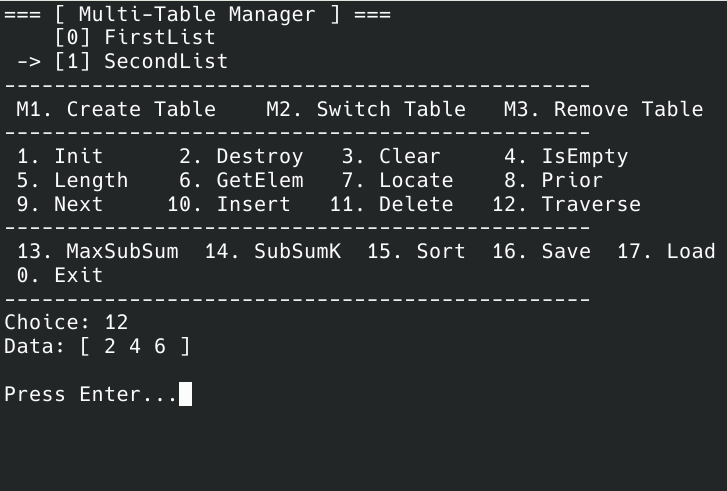
\includegraphics[width=0.6\textwidth]{assets/images/sq_test/l2.png}
	\caption{在 SecondList 中进行遍历操作，证实两表互不干扰}
	\label{fig:ts4_l2}
\end{figure}

通过 \texttt{M2} 命令切换回表 1，验证数据保持完整：
\begin{figure}[htbp]
	\centering
	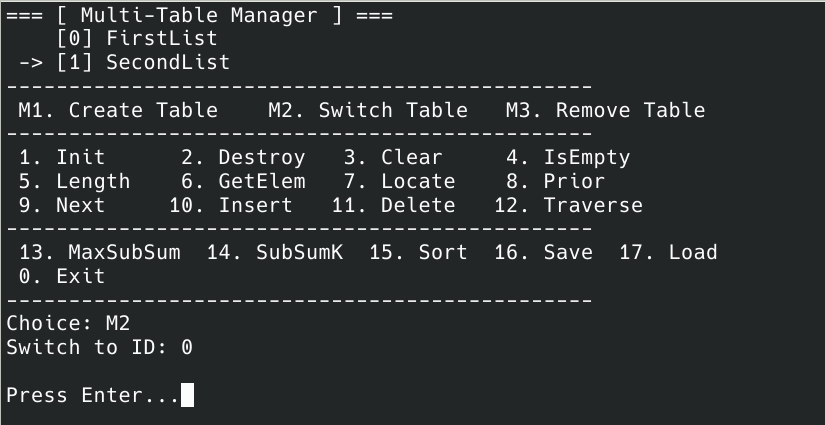
\includegraphics[width=0.6\textwidth]{assets/images/sq_test/l1_ing.png}
	\caption{发起向索引 0（FirstList）的切回操作}
	\label{fig:ts4_l1_ing}
\end{figure}
\begin{figure}[htbp]
	\centering
	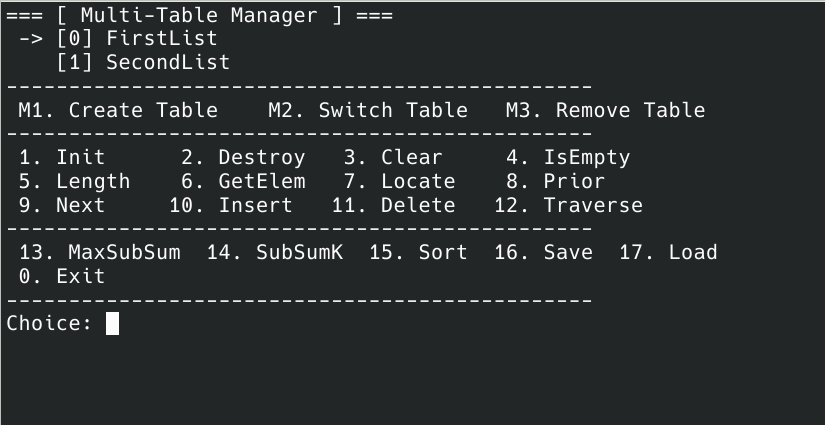
\includegraphics[width=0.6\textwidth]{assets/images/sq_test/l1_ed.png}
	\caption{当前激活的表再次变为 FirstList}
	\label{fig:ts4_l1_ed}
\end{figure}
\begin{figure}[htbp]
	\centering
	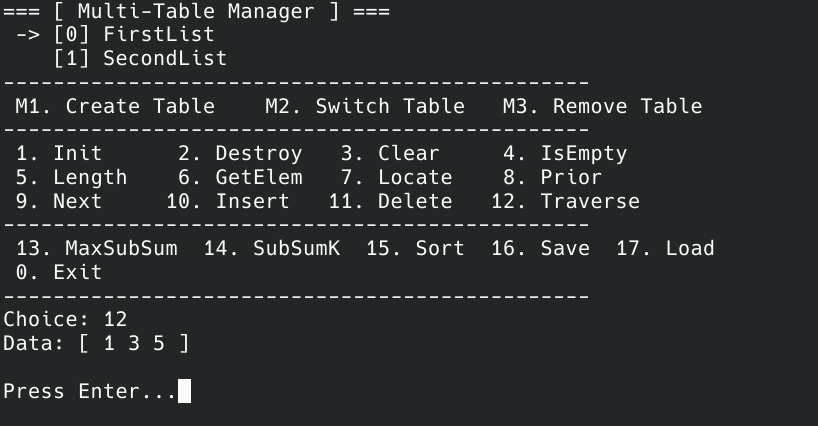
\includegraphics[width=0.6\textwidth]{assets/images/sq_test/l1_again.png}
	\caption{再次遍历 FirstList，其内部数据不受 SecondList 运行的影响}
	\label{fig:ts4_l1_again}
\end{figure}

测试销毁当前激活的表 1，系统应调用底层 \texttt{DestroyList} 回收内存，并将底层的 \texttt{tables} 向量前移：
\begin{figure}[htbp]
	\centering
	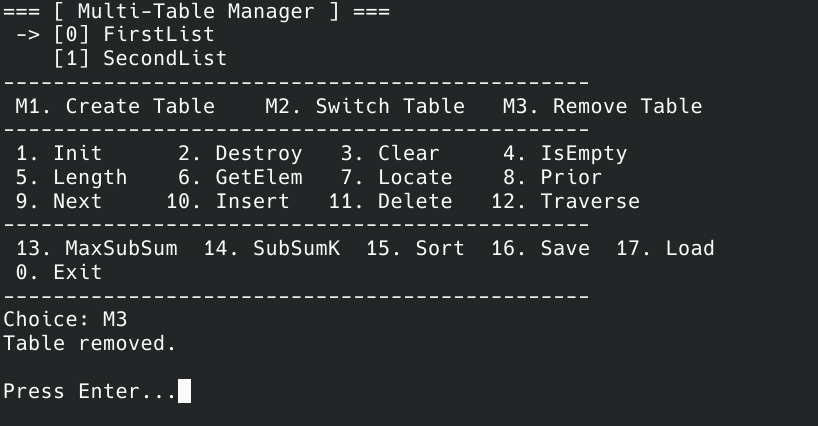
\includegraphics[width=0.6\textwidth]{assets/images/sq_test/del_l1_ing.png}
	\caption{执行 Remove Table (M3) 指令销毁 FirstList}
	\label{fig:ts4_del_l1_ing}
\end{figure}
\begin{figure}[htbp]
	\centering
	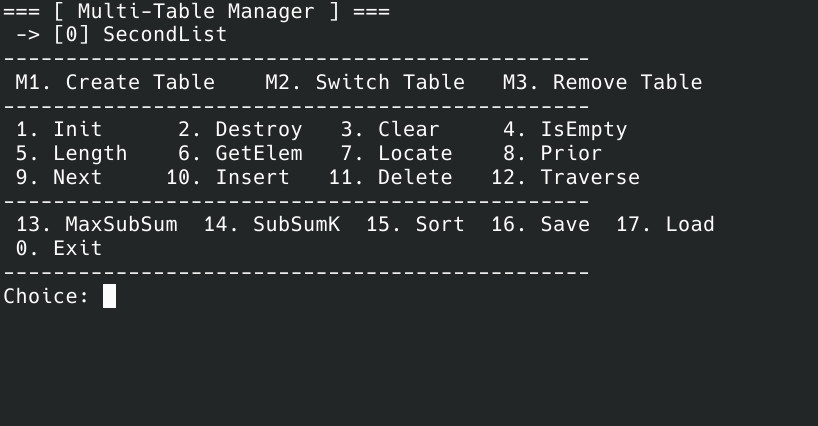
\includegraphics[width=0.6\textwidth]{assets/images/sq_test/del_l1_ed.png}
	\caption{销毁后管理视图更新：SecondList 自动前移至 0 索引，并被重新激活}
	\label{fig:ts4_del_l1_ed}
\end{figure}

最后进行边界测试，当尝试切换到一个超出范围的表索引（如表 1 已被删除，此时索引 1 越界）时：
\begin{figure}[htbp]
	\centering
	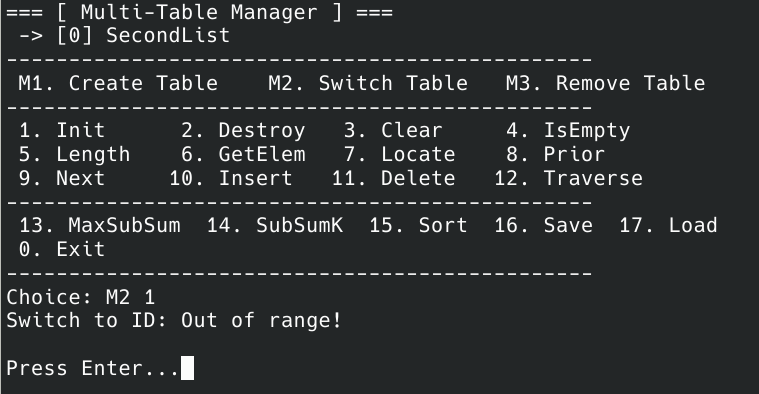
\includegraphics[width=0.6\textwidth]{assets/images/sq_test/cannot.png}
	\caption{越界切换保护：成功拦截对不存在的表实例的访问 (Out of range)}
	\label{fig:ts4_cannot}
\end{figure}

\newpage

\subsubsection{测试小结}
经过对四个维度的测试集的覆盖验证，本演示系统中的 20 项功能均达到了预期设计要求。
在常规的增删改查及文件保存测试中，系统表现出了良好的数据一致性；在附加算法测试中，无论是 $O(n)$ 复杂度的最大子串和求解，还是 Knuth 序列的希尔排序，均表现出了良好的性能；在多实例与异常边界测试中，系统自实现的防越界 \texttt{Panic} 机制以及基于枚举类型的 \texttt{Status} 状态码有效拦截了非法访问与未初始化操作，避免了段错误与内存泄漏的风险。测试结果证明了该程序逻辑的严谨性。

\subsection{实验小结}
本次实验不仅让我厘清了线性表的概念与基本运算，还让我从底层实现的角度（如自定义内存分配器 \texttt{std::allocator}、基于 \texttt{VectorTraits} 的索引偏移映射）理解了线性表物理地址连续性与逻辑位序之间的对应关系。

在系统开发与测试过程中，我遇到了一些工程问题。例如，\textbf{如何实现多表的独立管理与切换？} 没有采用容易污染命名空间的全局变量方案，而是设计了基于 \texttt{Vector<TableInstance>} 的管理结构和 \texttt{active\_idx} 索引机制，并利用 C++11 移动语义（\texttt{std::move}）避免了表实例切换和扩容时的冗余深拷贝，实现了多表的无开销切换。再如，\textbf{在实现排序功能时，如何避免自实现底层结构对标准库递归排序的依赖？} 如果直接调用带递归或借用堆栈的快速排序，有违从零手写底层结构的初衷。为此，我引入了基于 Knuth 增量序列的希尔排序，在确保底层代码独立性的同时达到了 $O(n^{1.11})$ 的较好性能。此外，利用魔数（Magic Number）进行二进制文件头校验，提升了程序 I/O 操作的安全性。

回顾整个实验过程，我认识到仅仅实现功能是不够的。在今后的实践中，我应当继续保持这种从数据结构底层出发的视角，去思考内存的精细管理、对象的生命周期以及泛型编程的扩展能力。同时，也应注意追求更低的时间复杂度（如本次实验中将 $O(n^2)$ 的最大子串和优化为 $O(n)$ 的动态规划实现）与较高的空间利用率，写出性能较好、健壮性较强的代码。

\newpage

\section{基于邻接表的图实现}
\subsection{问题描述}
图（Graph）是计算机科学中较为基础且表达能力较强的数据结构之一，用于表示物理或逻辑上具有"多对多"关联关系的对象集合。图本质上由顶点集（Vertex Set）和关系集（Edge/Arc Set）构成。在物理存储实现上，图主要分为邻接矩阵（顺序存储）和邻接表（链式存储）。邻接表通过为每个顶点维护一个单链表来记录其邻接点，在处理稀疏图时能节省内存空间。

本实验旨在构建一个交互式的图演示系统，通过命令行（CLI）驱动模式，完成图的基础运算（包括图的创建、销毁、顶点查找/赋值、增删顶点与弧、深度/广度优先遍历）以及附加功能（如求解距离小于 $K$ 的顶点集合、顶点间最短路径、连通分量计算等）的覆盖。同时，系统支持多图实例的统一管理与切换，集成了自定义文件格式的图保存与读取功能，通过完善的异常处理与结果展示，确保操作的健壮性与便捷性。

\begin{figure}[htbp]
	\centering
	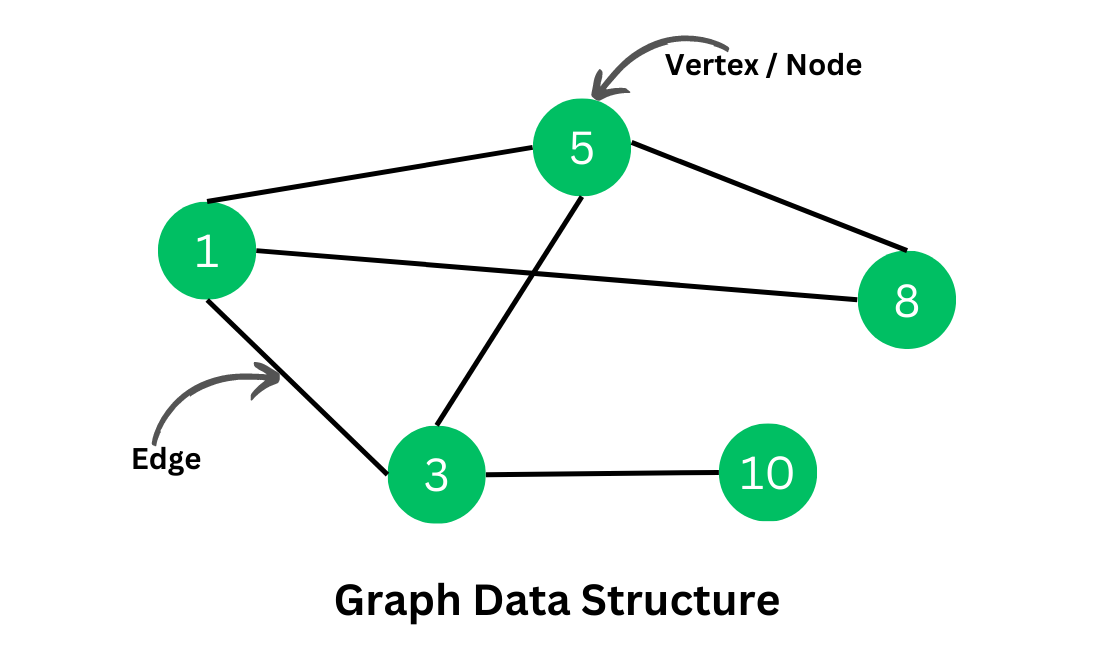
\includegraphics[width=0.6\textwidth]{assets/images/graph_st.png}
	\caption{基于邻接表的图逻辑结构示意图}
	\label{fig:graph_adjlist} % 这里的标签名是用来引用的
\end{figure}


\subsection{系统设计}

\subsubsection{头文件和封装}

\paragraph{1. 头文件 }
此为代码用到的标准库头文件，主要用于输入输出、字符串处理、动态数组（容器）、队列以及异常处理。

\newpage

\begin{lstlisting}[language=C++]
	#include <cstdio>
	#include <cstring>
	#include <stdexcept>
	#include <string>
	#include <vector>
	#include <queue>
	#include <utility>
\end{lstlisting}

\paragraph{ 2.数据结构封装 } 
此为代码对底层图结构的一次封装，没有使用纯粹的静态数组，而是利用\texttt{std::vector} 实现了动态邻接表。

\begin{lstlisting}[language=C++]
	namespace hust_ds::graph {
		/// 顶点的基础数据类型
		struct VertexType {
			int         key;      /// 唯一标识关键字
			std::string others;   /// 其他数据(负载)
		};
		
		/// 边表节点（弧）
		struct ArcNode {
			int      adjvex;      /// 该弧指向的顶点在顶点数组中的位序
			ArcNode* nextarc;     /// 指向下一条弧的指针
		};
		
		/// 顶点表节点
		struct VNode{
			VertexType data;      /// 顶点信息
			ArcNode*   firstarc;  /// 第一条依附该顶点的弧
		};
		
		/// 邻接表表示的图物理结构
		struct ALGraph{
			std::vector<VNode> vertices; /// 动态顶点表
			int arcnum;                  /// 图的边数
		};
		
		/// 顶点信息结束标志
		using Graph = ALGraph*;
		constexpr int DEF_END = -1; /// 图构建的结束标志
	}
\end{lstlisting}

\subsubsection{基本功能函数}

图的逻辑结构定义如下：\cite{yan2012data}
\begin{equation*}
	\text{ADT Graph} \{
	\begin{aligned}
		&\text{数据对象：} V = \{v_i \mid v_i \in \text{VertexSet}, i = 1, 2, \dots, n, n > 0\} \\
		&\text{数据关系：} VR = \{\langle v, w \rangle \mid v, w \in V\} \text{ (有向) 或 } (v, w) \text{ (无向)}
	\end{aligned}
	\}
\end{equation*}

遵循最小完备性与常用性相结合的原则，本实验实现了创建、销毁、遍历等12种基本操作，及5种附加操作：

\noindent
\begin{tabularx}{\textwidth}{p{4.5cm} X} % p{4.5cm}固定标签宽度，X自动适配剩余空间
	\textbf{CreateGraph(G,V,VR)} & 创建图：按给定的顶点集和关系集构造图（无向图），确保关键字唯一。 \\
	\textbf{DestroyGraph(G)} & 销毁图：释放图 $G$ 占用的全部内存空间。 \\
	\textbf{LocateVex(G,u)} & 查找顶点：返回关键字为 $u$ 的顶点在邻接表中的位序；不存在则返回 -1。 \\
	\textbf{PutVex(G,u,value)} & 顶点赋值：将关键字为 $u$ 的顶点信息更新为 $value$。 \\
	\textbf{FirstAdjVex(G,u)} & 首个邻接点：返回位序 $u$ 的顶点的第一个邻接顶点的位序。 \\
	\textbf{NextAdjVex(G,v,w)} & 下一个邻接点：返回位序 $v$ 顶点相对于位序 $w$ 的下一个邻接顶点位序。 \\
	\textbf{InsertVex(G,v)} & 插入顶点：在图 $G$ 中增加新顶点 $v$。 \\
	\textbf{DeleteVex(G,v)} & 删除顶点：删除图 $G$ 中关键字为 $v$ 的顶点及其关联的所有弧。 \\
	\textbf{InsertArc(G,v,w)} & 插入弧：在无向图中增加弧 $\langle v,w \rangle$ 及 $\langle w,v \rangle$。 \\
	\textbf{DeleteArc(G,v,w)} & 删除弧：在无向图中删除弧 $\langle v,w \rangle$ 及 $\langle w,v \rangle$。 \\
	\textbf{DFSTraverse(G,visit)} & 深度遍历：对图进行深度优先遍历，依次调用 \texttt{visit()}。 \\
	\textbf{BFSTraverse(G,visit)} & 广度遍历：对图进行广度优先遍历，依次调用 \texttt{visit()}。 \\
	\textbf{VerticesSetLessThanK} & 距离限值集：[附加] 返回与顶点 $v$ 距离小于 $k$ 的顶点集合。 \\
	\textbf{ShortestPathLength} & 最短路径：[附加] 返回顶点 $v$ 与顶点 $w$ 的最短路径长度。 \\
	\textbf{ConnectedComponents} & 连通分量：[附加] 统计并返回图的连通分量个数。 \\
	\textbf{SaveGraph/LoadGraph} & 文件存取：[附加] 将图保存至磁盘文件，或从文件中读取。 \\
	\textbf{CLI Multi-Graph} & 多图管理：[附加] 支持创建、切换、查找及移除多个图实例。 \\
\end{tabularx}

\subsection{系统实现}

\subsubsection{演示系统框架}
本系统没有采用传统的硬编码数字菜单，而是采用 \texttt{CLIApp} 类封装了一个类似 Shell 的命令行交互界面。通过 \texttt{std::getline} 获取用户的完整命令字符串，借助 \texttt{std::istringstream} 读取指令与参数，利用 \texttt{if-else} 路由到对应的底层图算法。
系统通过 \texttt{std::vector<GraphInstance> graphs} 管理多个图，\texttt{active\_idx} 指向当前激活的图。不仅支持 \texttt{create\_graph}、\texttt{switch\_graph} 进行多环境切换，还将所有底层 \texttt{throw std::runtime\_error} 抛出的异常在主循环的 \texttt{catch} 块中统一拦截并打印，提升了系统的容错能力和用户体验。

\subsubsection{数据结构设计}
系统的底层未使用定长数组，而是采用动态结构：

\textbf{1. 顶点基础与节点（VertexType / VNode / ArcNode）}：\texttt{VertexType} 抽象了负载，其中 \texttt{key} 是唯一的身份标识。\texttt{ArcNode} 是链表节点，仅记录目标顶点在数组中的位序(adjvex)以及下一条弧的指针。\texttt{VNode} 则是数组元素，包含了自身数据和出边链表的头指针 \texttt{firstarc}。

\textbf{2. 邻接表图（ALGraph）}：核心是一个基于 \texttt{C++ STL} 的 \texttt{std::vector<VNode> vertices} 动态数组。这样的设计使图具备了动态扩容的能力，也让 \texttt{DeleteVex} 等原本在静态数组中难以实现的操作得以方便地执行。

\subsubsection{函数思想及实现}
说明：为保证系统的健壮性，本实现中所有基本操作函数在执行实质逻辑前，均会进行指针判空与越界校验，若非法则直接 \texttt{throw} 标准异常，交由上层 UI 捕获。

\vspace{0.5em}
\noindent\textbf{1. 初始化与销毁图 (InitGraph / DestroyGraph)}
\newline\textbf{输入}：图指针的引用 (\texttt{Graph\&})
\newline\textbf{函数思想描述}：\texttt{InitGraph} 负责在堆区 \texttt{new} 一个 \texttt{ALGraph} 实例。\texttt{DestroyGraph} 则调用内部辅助函数 \texttt{detail::clear\_edges}，遍历 \texttt{vertices} 数组，利用 \texttt{while} 循环释放所有 \texttt{ArcNode} 链表节点的内存，最后 \texttt{delete G} 并将指针置空，避免内存泄漏。

\vspace{0.5em}
\noindent\textbf{2. 创建无向图 (CreateGraph)}
\newline\textbf{输入}：图引用 (\texttt{Graph\&})，顶点集数组 \texttt{V}，关系集数组 \texttt{VR}
\newline\textbf{函数思想描述}：首先清空当前图中可能的残余数据。遍历 \texttt{V}，校验 \texttt{key} 唯一性后将其 \texttt{emplace\_back} 存入 \texttt{vertices}。随后遍历关系集 \texttt{VR}，通过 \texttt{LocateVex} 获取 $v$ 和 $w$ 的位序。检查防自环、防重边后，利用**头插法**在位序 $v$ 和 $w$ 的单链表中分别插入一个新的 \texttt{ArcNode}，完成无向图的对称插入。

\vspace{0.5em}
\noindent\textbf{3. 查找与赋值 (LocateVex / PutVex)}
\newline\textbf{输入}：目标关键字 \texttt{u} 及新值 \texttt{value}
\newline\textbf{函数思想描述}：\texttt{LocateVex} 通过线性遍历 \texttt{vertices} 数组匹配 \texttt{key}，返回该顶点在数组中的索引（位序），若未找到返回 -1。\texttt{PutVex} 在赋值前进行逻辑校验：如果新值更改了 \texttt{key}，必须确保新 \texttt{key} 不会与图中其他顶点的 \texttt{key} 冲突，验证通过后直接覆写对应位序的 \texttt{data}。

\vspace{0.5em}
\noindent\textbf{4. 邻接点查询 (FirstAdjVex / NextAdjVex)}
\newline\textbf{输入}：顶点的位序 \texttt{u}，或相对邻接点位序 \texttt{v, w}
\newline\textbf{函数思想描述}：\texttt{FirstAdjVex} 直接通过索引访问 \texttt{vertices[u]}，返回其 \texttt{firstarc} 指向的 \texttt{adjvex}（若为空则返回 -1）。\texttt{NextAdjVex} 则需从 $v$ 的 \texttt{firstarc} 开始遍历单链表，直到找到 \texttt{adjvex == w} 的节点，然后返回其后继节点的 \texttt{adjvex}。

\vspace{0.5em}
\noindent\textbf{5. 插入与删除顶点 (InsertVex / DeleteVex)}
\newline\textbf{输入}：图引用 (\texttt{Graph\&})，顶点对象 \texttt{v} 或 关键字 \texttt{key}
\newline\textbf{函数思想描述}：\texttt{InsertVex} 校验唯一性后，直接调用 \texttt{std::vector::emplace\_back} 添加。
\texttt{DeleteVex} 是最复杂的基础操作。不仅需要释放待删除顶点自身的所有出边，还必须遍历**其余所有顶点**的边表，删除指向该顶点的弧。完成关系清理后，调用 \texttt{erase} 将其从 \texttt{vector} 中移除。
**核心难点**：由于底层使用了 \texttt{vector} 且中途删除了元素，原本在删除点之后的顶点的"位序"全部减 1。因此，算法最后必须进行一次全局修正，遍历所有边表，将所有 \texttt{adjvex > loc} 的值减 1，从而保持物理索引与逻辑拓扑的一致性。

\vspace{0.5em}
\noindent\textbf{6. 插入与删除弧 (InsertArc / DeleteArc)}
\newline\textbf{输入}：图引用 (\texttt{Graph\&})，关键字 \texttt{v, w}
\newline\textbf{函数思想描述}：\texttt{InsertArc} 查找到双方的位序后，采用头插法分别将对方加入自己的邻接表，并更新 \texttt{arcnum}。\texttt{DeleteArc} 采用经典的单链表删除节点逻辑（借助 \texttt{pre} 和 \texttt{p} 双指针），在 $v$ 的链表中删 $w$，在 $w$ 的链表中删 $v$。

\vspace{0.5em}
\noindent\textbf{7. 深度优先遍历 (DFSTraverse)}
\newline\textbf{输入}：图引用 (\texttt{Graph\&})，泛型访问器 \texttt{VisitFn\&\&}
\newline\textbf{函数思想描述}：借助辅助数组 \texttt{std::vector<bool> visited} 记录访问状态。通过内部静态结构体 \texttt{DFSHelper} 实现递归逻辑。外层使用循环遍历所有顶点，保证在非连通图的情况下，所有连通分量都能被深度优先递归遍历到。

\vspace{0.5em}
\noindent\textbf{8. 广度优先遍历 (BFSTraverse)}
\newline\textbf{输入}：图引用 (\texttt{Graph\&})，泛型访问器 \texttt{VisitFn\&\&}
\newline\textbf{函数思想描述}：基于 \texttt{std::queue<int>} 队列实现层序遍历。同样采用外层循环确保遍历所有非连通子图。访问某顶点后将其入队，在队列非空时弹出队头，并将其所有未访问的邻接点标记为已访问并压入队列。

\vspace{0.5em}
\noindent\textbf{9. [附加] 求距离小于 $K$ 的顶点集合 (VerticesSetLessThanK)}
\newline\textbf{输入}：起始顶点关键字 \texttt{v}，阈值 \texttt{k}
\newline\textbf{算法描述}：这是基于 BFS 算法的变体。队列中存储的不再是单一索引，而是 \texttt{std::pair<int, int>} \cite{cppref} 记录 \texttt{(当前位序, 距离)}。当弹出节点的距离小于 $k$ 时，将其加入结果集；若子节点距离预测 \texttt{dist + 1 >= k} 则进行剪枝，不再将其加入队列。

\vspace{0.5em}
\noindent\textbf{10. [附加] 最短路径长度 (ShortestPathLength)}
\newline\textbf{输入}：起点 \texttt{v} 和 终点 \texttt{w}
\newline\textbf{算法描述}：在无权图中，最短路径本质上就是广度优先遍历的层数。可以尝试利用 \texttt{std::queue<std::pair<int, int>>} 从起点逐层向外扩展，一旦在拓展下一层邻接点时发现目标 $w$，立即返回 \texttt{dist + 1}，实现了 $O(V+E)$ 复杂度的最短路求解。

\vspace{0.5em}
\noindent\textbf{11. [附加] 连通分量个数 (ConnectedComponentsNums)}
\newline\textbf{输入}：图引用 (\texttt{Graph\&})
\newline\textbf{算法描述}：遍历图的 \texttt{visited} 数组。每发现一个未被访问的节点，说明发现了一个新的连通分量，计数器 \texttt{+1}，并立即以此节点为起点触发一次 BFS，将该连通分量中的所有顶点标记为已访问。最终返回计数器值。

\vspace{0.5em}
\noindent\textbf{12. [附加] 文件保存与读取 (SaveGraph / LoadGraph)}
\newline\textbf{输入}：图引用 (\texttt{Graph\&})，文件路径字符串
\newline\textbf{函数思想描述}：

\textbf{保存（Save）}：采用结构化的文本格式保存。文件头写入自定义的魔数（Magic Number）\texttt{AGRH} 用于格式校验。接着写入顶点数与边数；随后按行写入每个顶点的 \texttt{key} 和 \texttt{others}；最后写入关系，利用 \texttt{-1} 作为每个顶点单链表邻接信息的结束符。

\textbf{加载（Load）}：读取文件魔数进行匹配，随后清理当前内存。按数量重建 \texttt{vertices}，最后在重构邻接表时，为了保持原有顺序，采用了尾插法维护 \texttt{tail} 指针，还原图的内存拓扑结构。

\vspace{0.5em}
\noindent\textbf{13. [附加] 多图管理功能}
\newline\textbf{输入}：用户命令行指令
\newline\textbf{函数思想描述}：在 \texttt{main.cpp} 中通过维护 \texttt{GraphInstance} 列表实现了多图。通过 \texttt{create\_graph} 创建新图并自动切换至该图，\texttt{switch\_graph} 支持索引或名称的双模查找切换；\texttt{remove\_graph} 在底层调用 \texttt{DestroyGraph} 避免内存泄漏后，结合 \texttt{std::vector::erase} 删除实例并自动调整当前激活索引。

\subsection{系统测试}
\subsubsection{测试环境与总体测试集设计}
系统的核心演示框架通过类 Shell 的命令行界面（CLI）进行交互。为了验证图 ADT（邻接表）各项基本功能及附加算法的正确性、健壮性和鲁棒性，本实验设计了 4 个维度的测试集进行交叉覆盖测试。由于采用标准输入流重定向解析机制，以下测试用例可直接作为文本块批量粘贴执行：

\begin{itemize}
	\item \textbf{测试集 1（基础构建与遍历测试）}：验证多图环境下的图实例创建、空图初始化，以及顶点/边关系的连续录入（\texttt{build}）。同时验证无向图对深度优先搜索（DFS）和广度优先搜索（BFS）层级逻辑的正确表达。
	\item \textbf{测试集 2（拓扑动态维护与关系查询）}：重点验证在运行态动态插入顶点、插入弧、删除顶点（联动边表删除）、删除弧操作。并检验更新顶点负载（\texttt{put}）、查询首个邻接点（\texttt{firstadj}）及后续邻接点（\texttt{nextadj}）是否能精准反映拓扑变化。
	\item \textbf{测试集 3（附加算法与文件存取）}：构造一个具有多条路径和多个非连通子图的图。验证连通分量计数、无权最短路径求解、距离小于 K 的顶点集提取等附加功能；同时测试将当前图保存至本地磁盘并完整读取加载的全流程。
	\item \textbf{测试集 4（多图管理与边界处理）}：测试同时挂载多个图环境，验证实例的切换及数据独立；并故意输入非法操作（如越界查找、重复节点构建、删除不存在的值），以验证系统的拦截与异常抛出机制。
\end{itemize}

\begin{figure}[htbp]
	\centering
	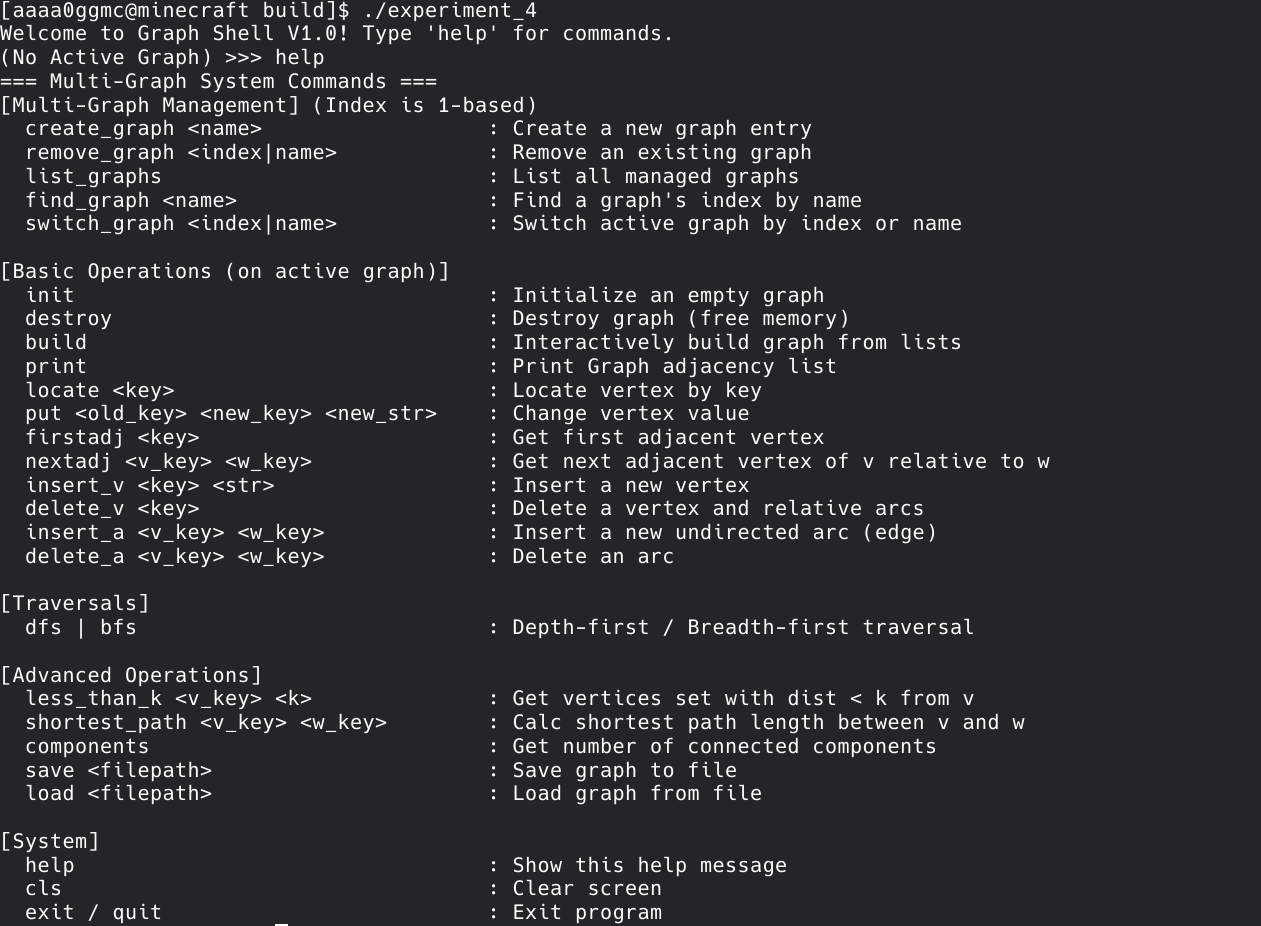
\includegraphics[width=1.0\textwidth]{assets/images/graph_menu.png}
	\caption{图演示系统的菜单}
	\label{fig:graph_menu} % 这里的标签名是用来引用的
\end{figure}


具体测试执行脚本流如下（注：此命令行执行序列严格遵循 CLI 解析规则）：

\paragraph{测试集 1} 基础构建与遍历测试
\begin{lstlisting}
	create_graph graph_base
	init
	build
	1 A 2 B 3 C 4 D 5 E -1 end
	1 2 1 3 2 4 3 5 -1 -1
	print
	dfs
	bfs
\end{lstlisting}

\paragraph{测试集 2} 拓扑动态维护与关系查询
\begin{lstlisting}
	create_graph graph_dynamic
	init
	build
	10 X 20 Y 30 Z -1 end
	10 20 20 30 -1 -1
	print
	insert_v 40 W
	insert_a 10 40
	print
	put 10 100 NEW_X
	firstadj 100
	nextadj 20 100
	delete_v 30
	delete_a 100 20
	print
\end{lstlisting}

\paragraph{测试集 3} 附加算法与文件存取
\begin{lstlisting}
	create_graph graph_adv
	init
	build
	1 N1 2 N2 3 N3 4 N4 5 N5 6 N6 -1 end
	1 2 2 3 1 3 4 5 -1 -1
	print
	components
	shortest_path 1 3
	less_than_k 1 3
	save graph_backup.txt
	destroy
	list_graphs
	load graph_backup.txt
	print
\end{lstlisting}

\paragraph{测试集 4} 多图管理与边界处理
\begin{lstlisting}
	create_graph env_A
	init
	create_graph env_B
	init
	switch_graph env_A
	insert_v 1 dataA
	switch_graph env_B
	insert_v 2 dataB
	print
	switch_graph env_A
	print
	locate 99
	firstadj 999
	insert_v 1 dup_data
	shortest_path 8 9
	list_graphs
	remove_graph env_A
	list_graphs
\end{lstlisting}

\subsubsection{测试集 1：基础构建与遍历测试}

本测试集旨在验证单图环境下的生命周期管理（创建与初始化）、批量图数据录入以及核心的深度优先与广度优先遍历算法的准确性。构建的测试用例如表 \ref{tab:graph_test_suite_1} 所示。

\begin{table}[htbp]
	\centering
	\caption{测试集 1 核心功能测试用例明细}
	\vspace{0.5em}
	\begin{tabular}{|>{\centering\arraybackslash}p{3cm}|>{\centering\arraybackslash}p{3.5cm}|>{\centering\arraybackslash}p{4.5cm}|c|}
		\hline
		\textbf{测试项} & \textbf{测试输入动作} & \textbf{预期结果} & \textbf{实际结果} \\ \hline
		建图与初始化 & 执行 \texttt{create\_graph} 与 \texttt{init} & 提示创建成功，分配内存空间 & 一致 \\ \hline
		批量顶点与弧录入 & \texttt{build} 输入 5 个顶点与 4 条边 & 成功建立邻接表，无向图对称插入 & 一致 \\ \hline
		邻接表结构打印 & 执行 \texttt{print} 打印邻接表 & 输出各顶点的出边表，拓扑结构吻合 & 一致 \\ \hline
		深度优先遍历 & 执行 \texttt{dfs} 遍历全图 & 沿着深度方向探索，输出 \texttt{1 3 5 2 4} & 一致 \\ \hline
		广度优先遍历 & 执行 \texttt{bfs} 遍历全图 & 按照层级逐层扩展，输出 \texttt{1 3 2 5 4} & 一致 \\ \hline
	\end{tabular}
	\label{tab:graph_test_suite_1}
\end{table}

\textbf{测试过程与验证：}
系统成功解析并执行了图的构建，建立的拓扑为：顶点 1 连接 2 和 3，顶点 2 连接 4，顶点 3 连接 5。在随后的 DFS 遍历中，系统优先探查深层节点；而在 BFS 遍历中，系统严格依照队列逻辑实现了层次遍历。运行输出与预期逻辑完全一致，如图 \ref{fig:graph_ts1} 所示。

\begin{figure}[htbp]
	\centering
	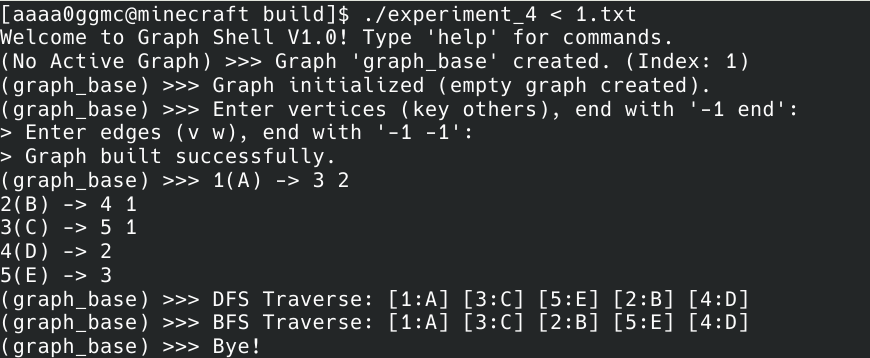
\includegraphics[width=0.8\textwidth]{assets/images/graphs/1.png}
	\caption{测试集 1 运行结果：图的基础构建与深度/广度遍历}
	\label{fig:graph_ts1}
\end{figure}

\subsubsection{测试集 2：拓扑动态维护与关系查询测试}

本部分重点验证底层 \texttt{std::vector} 与单链表结合时，动态增删操作的内存安全性以及节点关系位移的准确性。
初始录入节点 \texttt{10(X), 20(Y), 30(Z)} 及弧线。随后进行动态拓扑操作：
\begin{itemize}
	\item \textbf{动态增改：} 插入顶点 \texttt{40(W)} 并为其与 \texttt{10} 增加弧。利用 \texttt{put} 操作将 \texttt{10(X)} 更新为 \texttt{100(NEW\_X)}，数据顺利覆写。
	\item \textbf{邻接关系查询：} 查找顶点 \texttt{100} 的首个邻接点，准确返回 \texttt{40(W)}；查找顶点 \texttt{20} 相对于 \texttt{100} 的下一个邻接点，准确返回空（不存在）。
	\item \textbf{动态删减：} 删除顶点 \texttt{30}，系统不仅删除了该节点，还同时在 \texttt{20(Y)} 的邻接表中删除了指向 \texttt{30} 的残余弧，同时完成了全局位序修正。最后执行 \texttt{delete\_a} 移除弧线。
\end{itemize}

最终通过 \texttt{print} 输出的拓扑完全符合历经上述复杂操作后的终态，如图 \ref{fig:graph_ts2} 所示。

\begin{figure}[htbp]
	\centering
	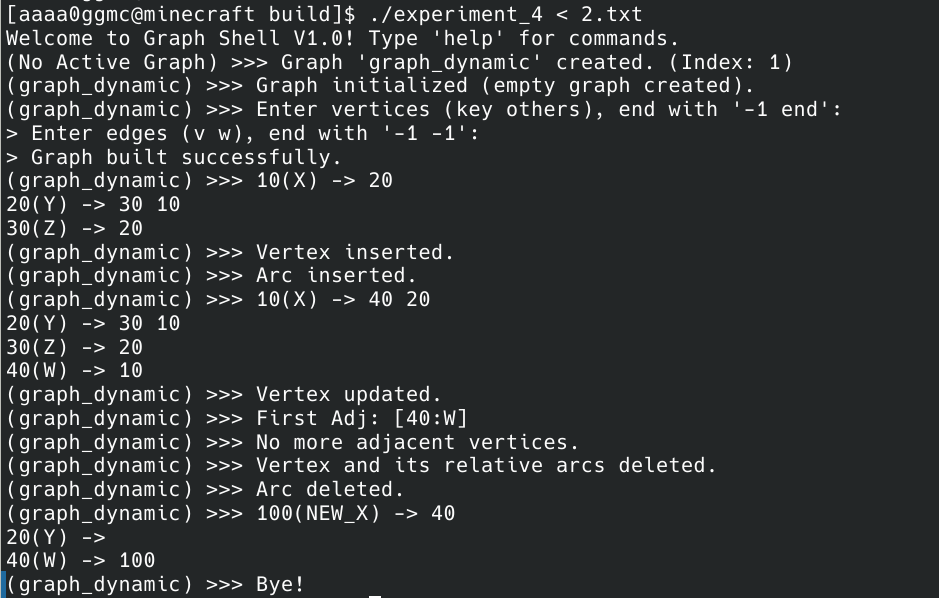
\includegraphics[width=0.8\textwidth]{assets/images/graphs/2.png}
	\caption{测试集 2 运行结果：顶点/弧的动态增删与节点关系查询}
	\label{fig:graph_ts2}
\end{figure}

\subsubsection{测试集 3：附加算法与文件存取测试}

为了测试系统对复杂非连通图的附加算法处理能力，构造了一个含有三个连通分量的图结构：节点 1,2,3 构成三角形连通块，节点 4,5 构成线段，节点 6 独立。

\begin{itemize}
	\item \textbf{附加算法：} 运行 \texttt{components} 成功统计出连通分量个数为 \textbf{3}。求解节点 1 到 3 的最短路径（\texttt{shortest\_path}）准确返回距离 \textbf{1}。提取距节点 1 距离小于 3 的顶点集合，准确返回了当前连通块内的 \texttt{1, 2, 3}。
	\item \textbf{保存与读取：} 利用 \texttt{save} 指令将当前复杂的图结构通过自定义的协议格式保存至 \texttt{graph\_backup.txt} 文件。随后通过 \texttt{destroy} 释放内存，确认 \texttt{list\_graphs} 表明图数据已清空。最后执行 \texttt{load} 读取该文件并 \texttt{print}，可见原有的拓扑及负载信息均被完整还原。
\end{itemize}

\begin{figure}[htbp]
	\centering
	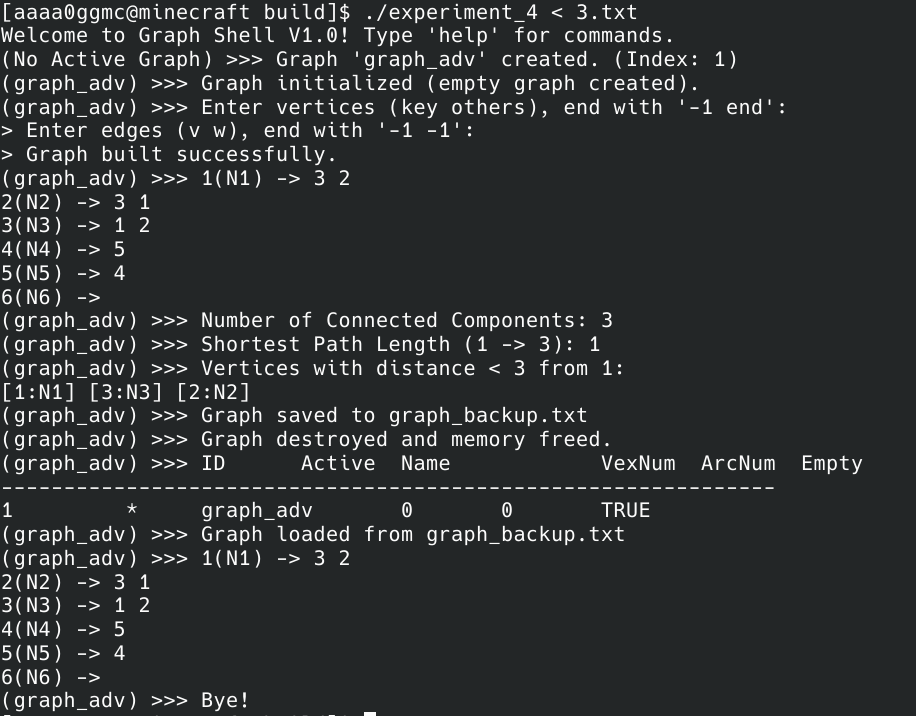
\includegraphics[width=0.8\textwidth]{assets/images/graphs/3.png}
	\caption{测试集 3 运行结果：连通分量/最短路径及文件存取}
	\label{fig:graph_ts3}
\end{figure}

\subsubsection{测试集 4：多图管理与边界处理测试}

健壮的系统需要能正确处理非法调用。本测试集在挂载两个独立图环境（\texttt{env\_A} 与 \texttt{env\_B}）的背景下，进行了多种异常测试：

\begin{itemize}
	\item \textbf{重复初始化检测：} 尝试对已存在的 \texttt{env\_A} 再次 \texttt{init}，系统正确捕获并抛出 \texttt{[Error] Graph is already inited}。
	\item \textbf{空指针越界检测：} 尝试在未初始化的 \texttt{env\_B} 中插入顶点，系统正确拦截 \texttt{[Error] Graph is null}，未发生段错误。
	\item \textbf{多环境隔离与键值防重：} 切换上下文互不干扰。在同一图中插入重复的 \texttt{key} 会触发唯一性校验 \texttt{Duplicate vertex key}。
	\item \textbf{无效查找拦截：} 查询图中不存在的顶点或者计算不存在节点的最短路径，均被 \texttt{Vertex not found} 异常捕获机制处理。
	\item \textbf{管理操作：} 执行 \texttt{remove\_graph} 销毁 \texttt{env\_A}，当前激活的图正确切换并更新管理视图。
\end{itemize}

\begin{figure}[htbp]
	\centering
	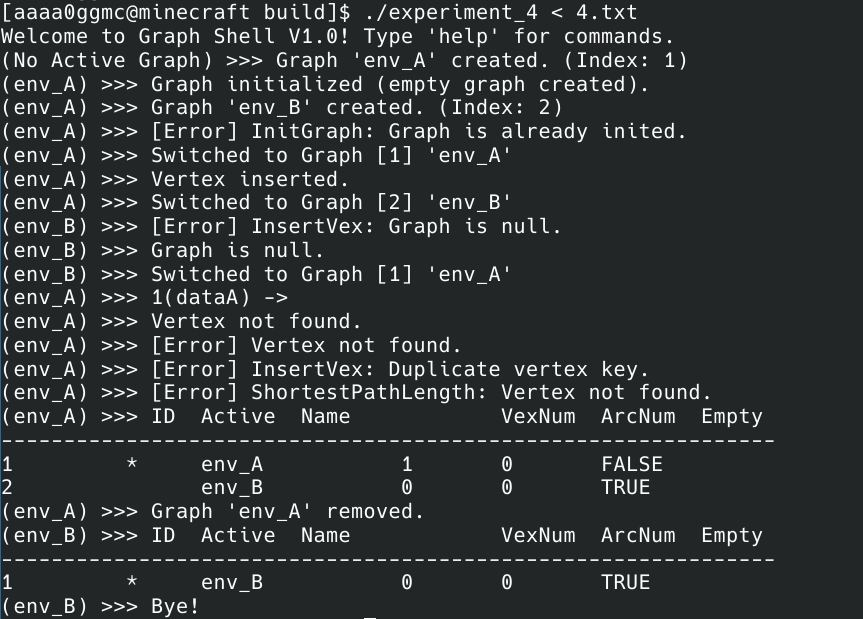
\includegraphics[width=0.8\textwidth]{assets/images/graphs/4.png}
	\caption{测试集 4 运行结果：多图环境切换与异常拦截}
	\label{fig:graph_ts4}
\end{figure}

\subsubsection{测试小结与功能实现清单}
经过四大维度的测试，本图演示系统顺利通过了所有的用例。底层代码中利用 C++ \texttt{std::runtime\_error} 与上层 \texttt{try-catch} 结合的架构发挥了较好作用，使得非法操作不会导致程序崩溃。同时，多图管理功能提升了系统的使用便利性和测试效率。所有 17 项要求的功能均完整实现并在本实验中验证通过，具体实现情况汇总如表 \ref{tab:feature_status} 所示。


\begin{table}[htbp]
	\centering
	\caption{图数据结构与算法演示系统总体功能实现清单}
	\vspace{0.5em}
	\setlength{\tabcolsep}{4pt}
	\renewcommand{\arraystretch}{1.15}
	\begin{tabular}{|l|l|c|p{5.2cm}|}
		\hline
		\textbf{功能模块} & \textbf{函数接口名称} & \textbf{完成状态} & \textbf{备注说明} \\ \hline
		\multirow{2}{*}{初始化与销毁} 
		& CreateGraph / InitGraph & $\checkmark$ & 具备重复建图与防自环机制 \\ \cline{2-4}
		& DestroyGraph & $\checkmark$ & 清理底层邻接表及动态内存区 \\ \hline
		
		\multirow{3}{*}{顶点与关系检索} 
		& LocateVex / PutVex & $\checkmark$ & 唯一性校验及信息重置 \\ \cline{2-4}
		& FirstAdjVex & $\checkmark$ & 基于单链表头指针快速检索 \\ \cline{2-4}
		& NextAdjVex & $\checkmark$ & 链表顺序遍历，鲁棒性良好 \\ \hline
		
		\multirow{2}{*}{动态拓扑维护} 
		& InsertVex / DeleteVex & $\checkmark$ & 附带自动连带删除及位序同步 \\ \cline{2-4}
		& InsertArc / DeleteArc & $\checkmark$ & 支持双向对称增删无向图弧段 \\ \hline
		
		\multirow{2}{*}{全图遍历} 
		& DFSTraverse & $\checkmark$ & 基于递归，可跨连通分量遍历 \\ \cline{2-4}
		& BFSTraverse & $\checkmark$ & 基于队列实现，防环路死循环 \\ \hline
		
		\multirow{3}{*}{附加算法} 
		& VerticesSetLessThanK & $\checkmark$ & 层序扩散附带深度剪枝算法 \\ \cline{2-4}
		& ShortestPathLength & $\checkmark$ & 基于 BFS 的 $O(V+E)$ 最短路 \\ \cline{2-4}
		& ConnectedComponentsNums & $\checkmark$ & 配合布尔向量全域扫描计数 \\ \hline
		
		\multirow{2}{*}{系统工程} 
		& SaveGraph / LoadGraph & $\checkmark$ & 自定义 AGRH 魔数头与尾插法重建 \\ \cline{2-4}
		& Multi-Graph CLI Shell & $\checkmark$ & 支持多图数据独立与命令行交互 \\ \hline
	\end{tabular}
	\label{tab:feature_status}
\end{table}

\newpage

\subsection{实验小结}
本次基于邻接表的图数据结构实验，是一次从线性逻辑向非线性拓扑逻辑跨越的重要实践。在本次实验中，我没有使用传统定长数组，而是采用 \texttt{std::vector} 动态数组结合单链表的复合物理结构，构建了一个支持动态扩容、健壮性较好的图 ADT。

在核心基本操作的实现中，我体会到了非线性数据结构状态维护的复杂性。尤其是 \texttt{DeleteVex}（删除顶点）操作，不仅需要释放自身的出边链表，还需全局扫描并删除其他顶点指向自身的弧；更具挑战的是，从动态数组中移除顶点会导致后续所有顶点的物理位序（索引）发生 $-1$ 的偏移，为此我专门设计了全局位序修正算法，确保了物理存储与逻辑拓扑的一致性。

在附加功能方面，我将图的基础遍历算法（DFS / BFS）进行了扩展应用：利用基于队列的层序扩展实现了无权图的最短路径求解及特定距离顶点集的提取；利用辅助布尔向量 \texttt{visited} 结合连通性探查实现了连通分量的精准统计。此外，通过引入自定义的 \texttt{AGRH} 文件魔数校验与尾插法重建机制，实现了复杂图结构的保存与读取。最后，配合基于命令行模式的多图管理界面，使得整个演示系统在算法实现的同时也具备较好的工程完整度。

\newpage

\section{课程的收获和建议}

\subsection{基于顺序存储结构的线性表实现}

\textbf{1. 实验收获：}
通过手写实现一个类似于 \texttt{std::vector} 的底层顺序表，我对其内部的内存管理机制有了较深入的理解。过去只知道调用标准库，现在我不仅掌握了动态两倍扩容（\texttt{capacity} 与 \texttt{length} 的关系）、内存的申请与释放，还学会了利用 C++11 的 \texttt{std::move} 移动语义来避免深拷贝，对元素插入和希尔排序的性能有所优化。
此外，为了兼容教材中从 $1$ 开始的逻辑位序与计算机从 $0$ 开始的物理内存位序，我引入了泛型编程中的 \texttt{VectorTraits} 机制，通过配置偏移量（\texttt{offset = -1}）解决了这一问题，锻炼了我的底层抽象封装能力。

\textbf{2. 课程建议：}
传统的顺序表实验指导书偏向于纯 C 语言风格（如使用 \texttt{malloc/free} 和 \texttt{Status} 宏定义）。建议在未来的课程设计中，可以适当鼓励或引入现代 C++（C++11/14/17）的特性，如模板（Template）、智能指针、结构化绑定（Structured Binding）以及 Lambda 表达式（如本次实验中的泛型 \texttt{visit} 遍历和 \texttt{compare} 比较）。这不仅能让代码更加安全清晰，也有助于学生更好地衔接现代工业界的数据结构开发标准。

\subsection{基于邻接表的图实现}

\textbf{1. 实验收获：}
图的实现拓宽了我的算法思维。我认识到邻接表作为一种适合稀疏图的物理结构，在快速获取顶点出边时较为高效，但在查询入边或删除顶点时却需要 $O(V+E)$ 的全局扫描代价，这让我理解了"数据结构需要针对具体场景进行选择"这一原则。
同时，本次图实验也提升了我的工程化代码组织能力。利用 \texttt{try-catch} 机制结合 \texttt{std::runtime\_error} 的抛出，我减少了过去到处判断错误码的冗余逻辑。底层算法遇到非法参数（如防自环、防重边、防越界）直接抛出异常，由最外层的 CLI UI 框架统一拦截并友好提示，使得程序遭遇非法输入时不会崩溃。

\textbf{2. 课程建议：}
实验指导书中要求利用传入 \texttt{V[]} 和 \texttt{VR[]} 静态数组的方式来初始化图，这在现代动态数据处理中显得不够灵活。
建议后续课程可以增加"通过标准格式文本文件（如类似 GraphML、JSON 或是自定义边表配置文本）来直接解析构建图"的要求，或者像本次系统一样要求实现一个交互式的命令流构建器。这样不仅能让学生掌握图的逻辑关系，还能同时锻炼字符串解析、流处理及状态机设计能力，使实验体系更具实用性与综合性。

\nocite{*} %% 作用是不对文献进行引用，但可以生成文献列表

\bibliographystyle{Experimental_Report}
\bibliography{Experimental_Report}
\setcounter{secnumdepth}{0}

\appendix
\section{附录A 共用代码}
\paragraph{alib5/algorithm/sort.h} 此头文件提供针对于RandomAccessIterator的较通用排序
\begin{lstlisting}
#ifndef ALIB5_ALGO_SORT_H_INCLUDED
#define ALIB5_ALGO_SORT_H_INCLUDED
#include <utility>
#include <iterator>

namespace alib5::algo::sort{
	template<class T> using default_compare = std::less<T>;
	template<class Fn> auto wrap_compare(Fn && fn){
		return [f = std::forward<decltype(fn)>(fn)]<class Tp>(const Tp & a,const Tp & b,bool reverse){
			return reverse ? f(b,a) : f(a,b);
		};
	}
	
	template<class Fn> auto wrap_inject(Fn && fn){
		return [f = std::forward<decltype(fn)>(fn)](std::size_t prev,std::size_t aft){
			if constexpr(!std::is_same_v<std::decay_t<decltype(f)>,std::nullptr_t>){
				f(prev,aft);
			}
		};
	}
	
	template<class Fn,class T> concept IsCompareFn = 
	requires(Fn && fn,const T& a,const T& b,bool & m){
		{ fn(a,b) } -> std::convertible_to<bool>;
	};
	template<class Fn> concept IsInjectFn = 
	requires(Fn && fn,std::size_t swap_prev,std::size_t swap_aft){
		fn(swap_prev,swap_aft);
	} || 
	requires(){
		std::is_same_v<std::decay_t<Fn>,std::nullptr_t>;
	};
	template<class T> concept IsIterator = 
	std::random_access_iterator<T> ||
	std::is_pointer_v<T>;
	
	template<class T> concept IsRandomAccessIterator = 
	std::random_access_iterator<T> ||
	std::is_pointer_v<T>;
	
	/// 支持随机访问和forward访问
	template<class T> concept IsGenericIterator = 
	std::forward_iterator<T> ||
	std::random_access_iterator<T> ||
	std::is_pointer_v<T>;
	
	enum class ShellGapType{
		Div2,
		Knuth,
		Hibbard
	};
	
	/// 简单的希尔排序 时间复杂度O(n^1.3) - O(n^2) Tier:D 
	/// 就是带上gap的插入排序
	template<ShellGapType GapType = ShellGapType::Div2,
	IsIterator IterType,
	IsCompareFn<typename std::iterator_traits<IterType>::value_type> CompareFn,
	IsInjectFn InjectFn = std::nullptr_t
	> 
	void shell(
	IterType begin,
	IterType end,
	CompareFn&& i_compare,
	bool reverse = false,
	InjectFn && i_inject = nullptr
	){
		using value_t = std::iterator_traits<IterType>::value_type;
		auto compare = wrap_compare(std::forward<CompareFn>(i_compare));
		auto inject = wrap_inject(std::forward<InjectFn>(i_inject));
		if(begin == end)return;
		
		size_t len = std::distance(begin,end);
		size_t gap = 1;
		
		if constexpr(GapType == ShellGapType::Div2){
			gap = len / 2;
		}else if constexpr(GapType == ShellGapType::Knuth){
			while(gap < len / 3)gap = 3 * gap + 1;
		}else if constexpr(GapType == ShellGapType::Hibbard){
			while(gap <= len) gap = (gap << 1) | 1;
			gap >>= 2;
			if(gap == 0)gap = 1;
		}
		
		auto gap_fn = [&](){
			if constexpr(GapType == ShellGapType::Div2) {
				gap >>= 1;
			}else if constexpr(GapType == ShellGapType::Knuth){
				gap = gap / 3;
			}else if constexpr(GapType == ShellGapType::Hibbard){
				gap >>= 1;
			}
		};
		
		while(gap > 0){
			for(size_t begin_pos = 0;begin_pos < gap;++begin_pos){
				for(size_t c_begin = begin_pos + gap;c_begin < len;c_begin += gap){
					IterType s_begin = begin + c_begin;
					IterType j = s_begin;
					value_t val = std::move(*s_begin);
					
					while(j > (begin + begin_pos) && compare(val,*(j - gap),reverse)){
						*j = std::move(*(j - gap));
						inject(std::distance(begin,j - gap),std::distance(begin,j));
						j -= gap;
					}
					*j = std::move(val);
				}
			}
			gap_fn();
		}
	}
}
#endif
\end{lstlisting}

\paragraph{alib5/ds/traits.h} 提供基础的定义(base.h仅包含了这个文件)
\begin{lstlisting}
#ifndef ALIB5_DS_TRAITS
#define ALIB5_DS_TRAITS
#include <type_traits>

namespace alib5::ds{
	/// 所有数据结构共有的traits
	struct BasicTraits{
		/// 发生错误的时候是否抛出异常
		bool throw_exception_instead_of_panic;
		
		constexpr BasicTraits(){
			throw_exception_instead_of_panic = false;
		}
	};
	
	
	/// 所有线性表共有的访问逻辑
	struct LinearListTraits : public BasicTraits{
		/// 偏移量，一般是0,也就是0-based访问，也可以是1-based
		/// 默认值：0 ，如果选择1-based,值为-1
		int offset;
		
		constexpr LinearListTraits(){
			offset = 0;
		}
	};
	
	/// 动态顺序表的traits
	struct VectorTraits : public LinearListTraits{
		/// 初始化/发生扩容的时候最小大小
		/// 用户可以硬性设置capacity为0，不过扩容的时候会选取max(min_capacity,capacity)
		/// 默认值: 4
		std::size_t min_capacity;
		
		constexpr VectorTraits(){
			min_capacity = 4;
		}
	};
	
	/// 链表traits
	struct ForwardListTraits : public LinearListTraits {
	};
};

#endif
\end{lstlisting}


\paragraph{alib5/ds/vector.h} 提供底层的Vector
\begin{lstlisting}
#ifndef ALIB5_DS_VECTOR
#define ALIB5_DS_VECTOR
#include <alib5/ds/base.h>
#include <alib5/adebug.h>
#include <type_traits>
#include <cstring>
#include <memory>

namespace alib5::ds{
	
	template<
	class T,
	VectorTraits traits = VectorTraits(),
	class Allocator = std::allocator<T> 
	>
	struct Vector{
		/// 这里实现通用的分配逻辑，可以更加方便地处理内存
		using value_type = T;
		using AllocatorTraits = std::allocator_traits<Allocator>;
		using Alloc = typename AllocatorTraits::template rebind_alloc<T>;
		
		Alloc allocator;
		
		Vector(const Allocator & alloc = Allocator()):allocator(alloc){}
		Vector(Allocator && alloc):allocator(std::move(alloc)){}
		
		/// 预留空间，capacity可以小于当前的capacity，效果等于shrink
		void reserve(size_t capacity);
		
		/// 确保至少有这么多空间，不会shrink只会扩增
		void ensure(size_t capacity){
			if(capacity > this->m_capacity){
				reserve(capacity);
			}
		}
		
		/// 重新设置大小,会把超过的数据直接截断，不影响capacity
		/// 后面的args为对每个对象构造的参数
		/// 要求： args均为copyable
		template<class... Args>
		void resize(size_t size,Args... args);
		
		//// 数据量大小关系
		/// 数据大小
		size_t size() const { return m_length; }
		size_t length() const { return size(); }
		/// 数据容量
		size_t capacity() const { return m_capacity; }
		/// 是否为空
		bool empty() const { return !size(); }
		/// 是否为满
		bool full() const { return size() == m_capacity; }
		
		/// 遍历上
		T* begin(){ return m_data; }
		T* end(){ return m_data + m_length; }
		const T* begin() const { return m_data; }
		const T* end() const { return m_data + m_length; }
		const T* cbegin() const { return m_data; }
		const T* cend() const { return m_data + m_length; }
		
		//// 查找函数，因为存入的数据没啥特征，所以时间复杂度为O(N)
		/// 返回指针，如果查询不到返回end()
		/// 这是通用版本，要求的comparefn第一个参数为const T&,第二个能接受Tp
		template<class Tp,class CompareFn>
		requires requires(const T& data,Tp & val,CompareFn & fn){ 
			{ fn(data,val) } -> std::convertible_to<bool>; 
		}
		const T* find(Tp && value,CompareFn && fn) const {
			for(const T& element : *this){
				if(fn(element,std::forward<Tp>(value)))return &element;
			}
			return end();
		}
		/// 非const版本
		template<class Tp,class CompareFn>
		requires requires(const T& data,Tp & val,CompareFn & fn){ 
			{ fn(data,val) } -> std::convertible_to<bool>; 
		}
		T* find(Tp && value,CompareFn && fn){
			return const_cast<T*>(((const Vector &)(*this)).find<Tp>(
			std::forward<Tp>(value),
			std::forward<CompareFn>(fn)
			));
		}
		
		/// 元素加入 & 插入
		/// 返回插入的指针
		T* insert(int index,T && value){
			return _insert(index + traits.offset, std::move(value));
		}
		T* insert(int index,const T & value){
			T v = value;
			return insert(index,std::move(v));
		}
		/// 这里支持迭代器
		T* insert(T* it,T && value){
			return _insert(it - begin(),std::move(value));
		}
		T* insert(T* it,const T & value){
			T v = value;
			return insert(it,std::move(v));
		}
		/// 往后面添加元素 O(1) 操作
		T* push_back(T && value){
			return _insert(m_length,std::move(value));
		}
		T* push_back(const T& value){
			T v = value;
			return _insert(m_length,std::move(v)); 
		}
		/// 往前面添加元素 O(L) 操作
		T* push_front(T && value){
			return _insert(0,std::move(value));
		}
		T* push_front(const T& value){
			T v = value;
			return _insert(0,std::move(v)); 
		}
		
		/// 元素的删除
		void erase(int index){
			_erase(index + traits.offset);
		}
		void erase(T* it){
			_erase(it - begin());
		}
		T remove(int index){
			T data = std::move((*this)[index]);
			_erase(index + traits.offset);
			return std::move(data);
		}
		T remove(T * it){
			return std::move(remove(it - begin()));
		}
		T pop_back(){
			return std::move(remove(end() - 1));
		}
		/// O(L) 操作
		T pop_front(){
			return std::move(remove(begin()));
		}
		/// 清除所有数控
		void clear(){
			if(!std::is_trivially_destructible_v<T>){
				for(size_t i = 0;i < m_length;++i){
					m_data[i].~T();
				}
			}
			m_length = 0;
		}
		
		//// 元素访问
		/// 访问不存在的index的时候返回nullptr
		T* at(int index){
			return _at(traits.offset + index);
		}
		const T* at(int index) const {
			return _at(traits.offset + index);
		}
		/// 编写访问
		const T& operator[](int index) const {
			const T * ptr = at(index);
			if(ptr)return *ptr;
			_panic_bounds(index);
			// 这里绝对不会被访问到，但是还是显示声明一下
			return *ptr;
		}
		T& operator[](int index){
			return const_cast<T&>(((const Vector &)(*this))[index]);
		}
		
		/// 这里都是基于0-based的方法，下划线开头
		const T* _at(int index) const {
			if(index < 0 || index >= m_length)return nullptr;
			return &m_data[index];
		}
		T* _at(int index){
			return const_cast<T*>(((const Vector &)(*this))._at(
			index
			));
		}
		// 插入新的元素
		T* _insert(int index,T && value);
		/// 删除对应位置的元素
		void _erase(int index);
		// index越界报错
		void _panic_bounds(int index) const {
			if constexpr(traits.throw_exception_instead_of_panic){
				throw std::out_of_range("Index out of bounds!");
			}else{
				panicf_if(index < 0,"The 0-based index({}) < 0.",index);
				panicf_if(index >= m_length,"The 0-based index({}) >= length({}).",index,m_length);
			}
		}
		
		/// @todo 也许我永远都不会做下面的几个功能了，等我用到了再做
		///     1. assgin
		///     2. insert
		
		/// 支持一下move
		Vector(Vector && vec){
			m_capacity = vec.m_capacity;
			m_data = vec.m_data;
			m_length = vec.m_length;
			
			vec.m_length = 0;
			vec.m_data = nullptr;
			vec.m_capacity = 0;
		}
		
		/// 支持一下copy
		Vector(const Vector & vec){
			reserve(vec.m_capacity);
			for(const T & element : vec){
				push_back(element);
			}
		}
		
		/// 析构函数，释放资源
		~Vector(){
			if(m_data){
				if constexpr(!std::is_trivially_destructible_v<T>){
					for(size_t i = 0;i < m_length;++i){
						m_data[i].~T();
					}
				}
				allocator.deallocate(m_data,m_capacity);
			}
		}
		private:
		/// 具体的数据
		T * m_data { nullptr };
		/// 数据预留大小
		size_t m_capacity { 0 };
		/// 当前数据的长度
		size_t m_length { 0 };
	};
}

namespace alib5::ds{
	template<
	class T,
	VectorTraits traits,
	class Allocator
	>
	template<
	class... Args
	>
	void Vector<T,traits,Allocator>::resize(size_t size,Args... args){
		ensure(size);
		// 如果非平凡，那么需要析构
		if constexpr(!std::is_trivial_v<T>){
			if(size < m_length){
				for(size_t i = size;i < m_length;++i){
					m_data[i].~T();
				}
			}
		}
		if(size > m_length){
			for(size_t i = m_length;i < size;++i){
				// 因为args要构造这么多次，本身要求就是要copyable，不然这不炸了吗？
				new (m_data + i) T(args...);
			}
		}
		m_length = size;
	}
	
	template<
	class T,
	VectorTraits traits,
	class Allocator
	>
	void Vector<T,traits,Allocator>::reserve(size_t new_capacity){
		// 也就是说支持在当前大小往下面shrink
		if(new_capacity > m_length && new_capacity != m_capacity){
			T * new_data = allocator.allocate(new_capacity);
			
			/// 如果复制操作时平凡的，使用memcpy一般会比其他情况更好？
			if constexpr(std::is_trivially_copyable_v<value_type>){
				if(m_data)std::memcpy(new_data,m_data,sizeof(value_type) * m_length);
			}else{
				for(size_t i = 0;i < m_length;++i){
					new (new_data + i) T(std::move(m_data[i]));
				}
				// 拆开不拆开一样的
				for(size_t i = 0;i < m_length;++i){
					m_data[i].~T();
				}
			}
			allocator.deallocate(m_data,m_capacity);
			
			// re-bind
			m_data = new_data;
			m_capacity = new_capacity;
		}
	}
	
	template<
	class T,
	VectorTraits traits,
	class Allocator
	>
	void Vector<T,traits,Allocator>::_erase(int index){
		if(index < 0 || index > m_length) [[unlikely]] _panic_bounds(index);
		if(index == m_length)return;
		
		// 析构这个位置，然后move后面的
		// 对于pop_back这种可以先move出去然后析构也不是问题
		if constexpr(!std::is_trivially_destructible_v<T>){
			m_data[index].~T();
		}
		
		if(index + 1 != m_length){
			for(int i = index + 1;i < m_length;++i){
				new (m_data + i - 1) T(std::move(m_data[i]));
			}
			
			// 最后一个位置有一个未初始化的数据
			if constexpr(!std::is_trivially_destructible_v<T>){
				m_data[m_length - 1].~T();
			}
		}
		
		m_length -= 1;
	}
	
	template<
	class T,
	VectorTraits traits,
	class Allocator
	>
	T* Vector<T,traits,Allocator>::_insert(int index,T && value){
		/// 排除错误情况
		// 这里是允许m_length这个位置的出现的
		if(index < 0 || index > m_length) [[unlikely]] _panic_bounds(index);
		
		T * focus_data = m_data;
		/// 这里是记录扩容
		size_t new_capacity = 0;
		
		// 考虑到性能原因，扩容移动一起做而不是使用ensure
		if(index + 1 > m_capacity){
			new_capacity = std::max(
			traits.min_capacity,
			(size_t)index + 1
			) * 2;
			
			T * new_data = allocator.allocate(new_capacity);
			
			// 对前面的数据进行迁移
			for(size_t i = 0;i < index;++i){
				new (new_data + i) T(std::move(m_data[i]));
			}
			
			m_data = new_data;
		}
		
		// 移动后面的数据
		for(int i = m_length - 1;i >= index; --i){
			new (m_data + i + 1) T(std::move(focus_data[i]));
		}
		
		new (m_data + index) T(std::move(value));
		m_length += 1;
		
		/// 这里是对于扩容的对象进行清理
		if(new_capacity) [[unlikely]] {
			// 析构focus_data旧的位置的数据
			if constexpr(!std::is_trivially_destructible_v<T>){
				// 前面已经加了个1可，因此这里减回来
				size_t old_length = m_length - 1;
				for(size_t i = 0;i < old_length;++i){
					focus_data[i].~T();
				}
			}
			allocator.deallocate(focus_data,m_capacity);
			// 最后设置capacity
			m_capacity = new_capacity;
		}
		
		return m_data + index;
	}
}

#endif
\end{lstlisting}

\paragraph{alib5/ds/forward\_list.h} 提供一个单链表的基础数据结构
\begin{lstlisting}
#ifndef ALIB5_DS_FWD_LIST
#define ALIB5_DS_FWD_LIST
#include <alib5/ds/base.h>
#include <alib5/adebug.h>
#include <memory>
#include <utility>
#include <stdexcept>
#include <concepts>

namespace alib5::ds{
	
	template<
	class T,
	ForwardListTraits traits = ForwardListTraits(),
	class Allocator = std::allocator<T>
	>
	class ForwardList{
		public:
		using value_type = T;
		
		struct Node {
			T data;
			Node* next;
			template<class... Args>
			Node(Args&&... args) : data(std::forward<Args>(args)...), next(nullptr) {}
		};
		
		using AllocatorTraits = std::allocator_traits<Allocator>;
		using NodeAlloc = typename AllocatorTraits::template rebind_alloc<Node>;
		
		NodeAlloc allocator;
		Node* m_head { nullptr };
		
		private:
		template<class... Args>
		Node* create_node(Args&&... args){
			Node* node = allocator.allocate(1);
			std::allocator_traits<NodeAlloc>::construct(allocator, node, std::forward<Args>(args)...);
			return node;
		}
		
		void destroy_node(Node* node){
			std::allocator_traits<NodeAlloc>::destroy(allocator, node);
			allocator.deallocate(node, 1);
		}
		public:
		ForwardList(const Allocator& alloc = Allocator()) : allocator(alloc) {}
		ForwardList(Allocator&& alloc) : allocator(std::move(alloc)) {}
		
		~ForwardList(){
			clear();
		}
		
		/// 不断往下探，情况后面的数据
		void clear(){
			Node* curr = m_head;
			while(curr){
				Node* next = curr->next;
				destroy_node(curr);
				curr = next;
			}
			m_head = nullptr;
		}
		
		bool empty() const {
			return m_head == nullptr;
		}
		
		size_t size() const {
			size_t len = 0;
			for (Node* p = m_head; p; p = p->next) {
				++len;
			}
			return len;
		}
		size_t length() const { return size(); }
		
		T* at(int index){
			return _at(index + traits.offset);
		}
		const T* at(int index) const {
			return _at(index + traits.offset);
		}
		
		const T& operator[](int index) const {
			const T* ptr = at(index);
			if (ptr) return *ptr;
			_panic_bounds(index + traits.offset);
			return *ptr;
		}
		T& operator[](int index){
			return const_cast<T&>(((const ForwardList&)(*this))[index]);
		}
		
		/// 基于 0-based 的内部访问
		const T* _at(int index) const {
			if (index < 0) return nullptr;
			Node* p = m_head;
			for (int i = 0; i < index && p; ++i) p = p->next;
			return p ? &(p->data) : nullptr;
		}
		T* _at(int index){
			return const_cast<T*>(((const ForwardList&)(*this))._at(index));
		}
		
		template<class Tp, class CompareFn>
		requires requires(const T& data, Tp& val, CompareFn& fn){ 
			{ fn(data, val) } -> std::convertible_to<bool>; 
		}
		const T* find(Tp&& value, CompareFn&& fn) const {
			for (Node* p = m_head; p; p = p->next) {
				if (fn(p->data, std::forward<Tp>(value))) return &(p->data);
			}
			return nullptr;
		}
		template<class Tp, class CompareFn>
		T* find(Tp&& value, CompareFn&& fn) {
			return const_cast<T*>(((const ForwardList&)(*this)).find<Tp>(
			std::forward<Tp>(value),
			std::forward<CompareFn>(fn)
			));
		}
		
		/// 获得前驱
		bool prior_elem(const T& cur_e, T& pre_e) const {
			if (!m_head || !m_head->next) return false;
			Node* p = m_head;
			while (p->next) {
				if (p->next->data == cur_e) {
					pre_e = p->data;
					return true;
				}
				p = p->next;
			}
			return false;
		}
		
		/// 获得后继 NextElem
		bool next_elem(const T& cur_e, T& next_e) const {
			Node* p = m_head;
			while(p && p->next){
				if(p->data == cur_e){
					next_e = p->next->data;
					return true;
				}
				p = p->next;
			}
			return false;
		}
		
		/// 插入元素 ListInsert (应用 offset)
		Node* insert(int index, T&& value){
			return _insert(index + traits.offset, std::move(value));
		}
		Node* insert(int index, const T& value){
			T v = value;
			return insert(index, std::move(v));
		}
		
		/// 往头部和尾部添加元素的便捷方法
		Node* push_front(T&& value){ return _insert(0, std::move(value)); }
		Node* push_front(const T& value){ T v = value; return _insert(0, std::move(v)); }
		
		T remove(int index){
			return _erase(index + traits.offset);
		}
		T pop_front(){
			return _erase(0);
		}
		
		template<class VisitFn>
		void traverse(VisitFn&& visit) const {
			for (Node* p = m_head; p; p = p->next) {
				visit(p->data);
			}
		}
		
		void reverse(){
			Node* prev = nullptr;
			Node* curr = m_head;
			while (curr) {
				Node* next = curr->next;
				curr->next = prev;
				prev = curr;
				curr = next;
			}
			m_head = prev;
		}
		
		void remove_nth_from_end(int n){
			if (n <= 0 || !m_head) return;
			Node** slow = &m_head;
			// 记录“尾部”
			Node* fast = m_head;
			for(int i = 0; i < n; ++i){
				if (!fast) return; // 不足 n 个
				fast = fast->next;
			}
			while(fast){
				fast = fast->next;
				slow = &((*slow)->next);
			}
			Node* to_delete = *slow;
			*slow = to_delete->next;
			destroy_node(to_delete);
		}
		
		/// 链表排序 sortList (Bubble Sort 纯交换指针区域)
		template<class CompareFn>
		void sort(CompareFn&& cmp){
			if(!m_head || !m_head->next) return;
			bool swapped;
			Node* end_node = nullptr;
			do{
				swapped = false;
				Node** curr = &m_head;
				
				while(*curr && (*curr)->next && (*curr)->next != end_node){
					Node* a = *curr;
					Node* b = a->next;
					
					if(cmp(b->data, a->data)){ 
						// 断开原链接，重新连接达到交换效果，不移动 data
						a->next = b->next;
						b->next = a;
						*curr = b;
						swapped = true;
					}
					curr = &((*curr)->next);
				}
				end_node = *curr;
			} while (swapped);
		}
		
		Node* _insert(int index, T&& value);
		T _erase(int index);
		
		void _panic_bounds(int index) const {
			if constexpr(traits.throw_exception_instead_of_panic){
				throw std::out_of_range("Index out of bounds!");
			}else{
				panicf_if(index < 0, "The 0-based index({}) < 0.", index);
				panicf_if(true, "The 0-based index({}) is out of bounds.", index);
			}
		}
	};
}

namespace alib5::ds{
	template<
	class T,
	ForwardListTraits traits,
	class Allocator
	>
	typename ForwardList<T, traits, Allocator>::Node* 
	ForwardList<T, traits, Allocator>::_insert(int index, T&& value){
		if(index < 0) [[unlikely]] _panic_bounds(index);
		
		if(index == 0){
			Node* new_node = create_node(std::move(value));
			new_node->next = m_head;
			m_head = new_node;
			return m_head;
		}
		
		Node* p = m_head;
		for(int i = 0; i < index - 1 && p; ++i){
			p = p->next;
		}
		
		if(!p) [[unlikely]] _panic_bounds(index);
		
		Node* new_node = create_node(std::move(value));
		new_node->next = p->next;
		p->next = new_node;
		return new_node;
	}
	
	template<
	class T,
	ForwardListTraits traits,
	class Allocator
	>
	T ForwardList<T, traits, Allocator>::_erase(int index) {
		if(!m_head || index < 0) [[unlikely]] _panic_bounds(index);
		
		if(index == 0){
			Node* to_delete = m_head;
			m_head = m_head->next;
			T data = std::move(to_delete->data);
			destroy_node(to_delete);
			return data;
		}
		
		Node* p = m_head;
		for(int i = 0; i < index - 1 && p->next; ++i){
			p = p->next;
		}
		
		if(!p->next) [[unlikely]] _panic_bounds(index);
		
		Node* to_delete = p->next;
		p->next = to_delete->next;
		T data = std::move(to_delete->data);
		destroy_node(to_delete);
		
		return data;
	}
	
}
#endif
\end{lstlisting}

\paragraph{alib5/ds/bin\_tree.h} 提供基础的二叉树结构
\begin{lstlisting}
#ifndef ALIB5_DS_BIN_TREE
#define ALIB5_DS_BIN_TREE
#include <iostream>

namespace alib5::ds{
	template<class T>
	struct BinTree{
		/// 实际上保存的数据
		T data;
		
		/// 左边左边，个人不习惯lchild,rchild，不如left right
		BinTree<T> * left = nullptr;
		/// 右边
		BinTree<T> * right = nullptr;
		
		/// 给自己数据赋值
		void set(T & value){
			data = value;
		}
		
		/// 给左边赋值，自动创建新的
		void set_left(T & value){
			if(!left)left = new BinTree<T>;
			left->data = value;
		}
		
		/// 给右边赋值，自动创建新的
		void set_right(T & value){
			if(!right)right = new BinTree<T>;
			right->data = value;
		}
		
		/// 左边是否是空的，为啥没有empty()呢，因为根节点本来就不是空的了
		bool left_empty(){
			return left == nullptr;
		}
		
		bool right_empty(){
			return right == nullptr;
		}
		
		/// 计算深度，使用递归的DFS
		int depth(int base = 1){
			int left_max = base;
			int right_max = base;
			
			if(left)left_max = left->depth(base + 1);
			if(right)right_max = right->depth(base + 1);
			
			return std::max(left_max,right_max);
		}
		
		void clear_left(){
			if(left){
				left->clear_left();
				left->clear_right();
				
				delete left;
				left = nullptr;
			}else throw std::runtime_error("Left node is empty");
			// 我觉得还是干脆抛出异常吧，省心一点
		}
		
		void clear_right(){
			if(right){
				right->clear_left();
				right->clear_right();
				
				delete right;
				right = nullptr;
			}else throw std::runtime_error("Right node is empty");
		}
	};
}

#endif
\end{lstlisting}
\newpage

\section{附录B 基于顺序存储结构线性表实现的源程序}
\paragraph{hust\_ds/sq\_list.h} ADT封装
\begin{lstlisting}
	#ifndef HUST_DS_SQ_LIST_H
	#define HUST_DS_SQ_LIST_H
	#include <alib5/ds/vector.h>
	#include <alib5/aalgorithm.h>
	
	namespace hust_ds::sq_list{
		using namespace alib5::ds;
		constexpr VectorTraits traits = [](){
			VectorTraits traits;
			// 1-based index support
			traits.offset = -1;
			return traits;
		}();
		
		using Type = int;
		using Allocator = std::allocator<int>;
		using Container = Vector<int,traits,Allocator>;
		using List = Container*;
		
		enum class Status : int {
			Infeasible = -1,
			OK = 0,
			Error = 1,
		};
		
		inline Status InitList(List& list){
			using enum Status;
			if(list)return Infeasible;
			list = new Container();
			return OK;
		}
		
		inline Status DestroyList(List& list){
			using enum Status;
			if(!list)return Infeasible;
			delete list;
			list = nullptr;
			return OK;
		}
		
		inline Status ClearList(List& list){
			using enum Status;
			if(!list)return Infeasible;
			list->clear();
			return OK;
		}
		
		inline std::pair<bool,Status> ListEmpty(List & list){
			using enum Status;
			if(!list)return {false,Infeasible};
			return {list->empty(),OK};
		}
		
		inline int ListLength(List & list){
			if(!list)return -1;
			return static_cast<int>(list->length());
		}
		
		inline Status GetElem(List & list,int i,Type & e){
			using enum Status;
			if(!list)return Infeasible;
			Type * ptr = list->at(i);
			if(!ptr)return Error;
			e = *ptr;
			return OK;
		}
		
		template<class CompareFn>
		inline int LocateElem(List & list,Type e,CompareFn && compare){
			if(!list)return 0;
			Type * ptr = list->find(e,std::forward<CompareFn>(compare));
			if(ptr == list->end())return 0;
			// 反算 1-based index: ptr - begin() - offset
			return static_cast<int>(ptr - list->begin() - traits.offset);
		}
		
		inline Status PriorElem(List & list,Type cur_e,Type & pre_e){
			using enum Status;
			if(!list)return Infeasible;
			// 查找第一个匹配项
			Type * ptr = list->find(cur_e,[](const Type& a,const Type& b){return a == b;});
			if(ptr == list->end() || ptr == list->begin())return Error;
			pre_e = *(ptr - 1);
			return OK;
		}
		
		inline Status NextElem(List & list,Type cur_e,Type & next_e){
			using enum Status;
			if(!list)return Infeasible;
			Type * ptr = list->find(cur_e,[](const Type& a,const Type& b){return a == b;});
			if(ptr == list->end() || ptr + 1 == list->end())return Error;
			next_e = *(ptr + 1);
			return OK;
		}
		
		inline Status ListInsert(List & list,int i,Type e){
			using enum Status;
			if(!list)return Infeasible;
			// Vector内部会处理 offset 并在越界时 panic 或 throw
			// 1-based index: i=1 对应 offset=-1 后的 0
			list->insert(i,e);
			return OK;
		}
		
		inline Status ListDelete(List & list,int i,Type & e){
			using enum Status;
			if(!list)return Infeasible;
			if(i < 1 || i > (int)list->length())return Error;
			e = list->remove(i);
			return OK;
		}
		
		template<class VisitFn>
		inline Status ListTraverse(List & list,VisitFn && visit){
			using enum Status;
			if(!list)return Infeasible;
			for(auto & element : *list){
				visit(element);
			}
			return OK;
		}
		
		inline int MaxSubArray(List& list){
			if(!list || list->empty())return 0;
			
			// 不断计算累加和
			int max_val = (*list)[1];
			int curr_max = (*list)[1];
			for(size_t i = 2;i <= list->length();++i){
				// 如果list[i] < 0那么此时我重新开始算的话收益反而更低
				// 因此应该保留，类似 -1 1 2 3 4 -1 5 
				// 到第二个-1时如果抛弃就只有-1了
				curr_max = std::max((*list)[i], curr_max + (*list)[i]);
				max_val = std::max(max_val, curr_max);
			}
			return max_val;
		}
		
		inline int SubArrayNum(List& list, int k){
			if(!list || list->empty()) return 0;
			size_t len = list->length();
			
			// 复用 Container 存储前缀和 P[0...len]
			// p[1] 对应 P[0] = 0, p[2] 对应 P[1]...
			Container p; p.resize(len + 1, 0);
			for(size_t i = 1; i <= len; ++i) 
			p[i+1] = p[i] + (*list)[i];
			
			int count = 0;
			// 双重循环找差值为 k 的两项
			for(size_t j = 1; j <= len; ++j)for(size_t i = 0; i < j; ++i)
			if(p[j+1] - p[i+1] == k){
				count++;
			}
			return count;
		}
		
		inline Status SortList(List& list){
			if(!list)return Status::Infeasible;
			// 使用希尔排序
			// 原因： 因为快排我这里面用到了std::vector模拟堆栈
			// 这在数据结构里面应该是鸡和蛋的问题，所以使用几乎无状态
			// 同时效率也不错的shell排序是更好的选择
			// 经过测试Knuth的时间复杂度在2^20左右的数据量下约为 O(N^1.1132945334842599)，因此还挺好
			// 对比之下快排(三数取中 + Hoare分区)是 O(N^1.0120299377159614)
			alib5::algo::sort::shell<alib5::algo::sort::ShellGapType::Knuth>(
			list->begin(),
			list->end(),
			std::less<Type>()
			);
			return Status::OK;
		}
		
		/// 文件特征 SEQL[Length][SizeofType][Data...]
		/// 这里的SizeofType是拿来校验的
		inline Status SaveList(List& list, const char* filename){
			if(!list)return Status::Infeasible;
			
			FILE* fp = fopen(filename, "wb");
			if(!fp)return Status::Error;
			// 特殊序列，只要是为了保证没有读错文件然后boom
			fwrite("SEQL", 1, 4, fp);
			
			size_t len = list->length();
			size_t sz = sizeof(Type);
			
			fwrite(&len, sizeof(size_t), 1, fp);
			fwrite(&sz, sizeof(size_t), 1, fp);
			fwrite(list->begin(), sz, len, fp);
			fclose(fp);
			return Status::OK;
		}
		
		inline Status LoadList(List& list, const char* filename){
			if(!list)return Status::Infeasible;
			
			FILE* fp = fopen(filename, "rb");
			if(!fp)return Status::Error;
			
			char magic[4]; 
			fread(magic, 1, 4, fp);
			if(memcmp(magic, "SEQL", 4) != 0){ 
				fclose(fp); 
				return Status::Error; 
			}
			
			size_t len, sz;
			
			fread(&len, sizeof(size_t), 1, fp);
			fread(&sz, sizeof(size_t), 1, fp);
			
			if(sz != sizeof(Type)){
				fclose(fp); 
				return Status::Error; 
			}
			
			list->clear(); 
			list->resize(len);
			
			fread(list->begin(), sz, len, fp);
			fclose(fp);
			return Status::OK;
		}
	}
	
	#endif
\end{lstlisting}

\paragraph{main.cpp} 主程序
\begin{lstlisting} 
	#include <iostream>
	#include <string>
	#include <limits>
	#include <hust_ds/sq_list.h>
	
	using namespace hust_ds::sq_list;
	
	struct TableInstance{
		Vector<char> name;
		List list = nullptr;
		
		// 默认构造，Vector内部会自行初始化
		TableInstance() = default;
		// 为了方便 Vector 扩容时的搬运
		TableInstance(TableInstance&&) = default;
	};
	
	class App{
		private:
		// 管理层也使用自家的 Vector
		Vector<TableInstance> tables;
		int active_idx = -1;
		
		void pause(){
			std::cout << "\nPress Enter...";
			std::cin.ignore(std::numeric_limits<std::streamsize>::max(), '\n');
			std::cin.get();
		}
		
		List& curr(){
			return tables._at(active_idx)->list; 
		}
		
		// 辅助：将 std::string 转为 Vector<char>
		void set_name(Vector<char>& vec, const std::string& str){
			vec.clear();
			for(char c : str) vec.push_back(c);
			vec.push_back('\0'); // 方便后续逻辑或调试
		}
		
		// 辅助：打印 Vector<char>
		void print_name(const Vector<char>& vec){
			for(const char& c : vec) if(c != '\0') std::cout << c;
		}
		
		public:
		void run(){
			std::string cmd;
			while(true){
				system("cls || clear");
				std::cout << "=== [ Multi-Table Manager ] ===\n";
				if(tables.empty()) std::cout << " (No tables created)\n";
				else {
					for(int i = 0; i < (int)tables.size(); ++i){
						std::cout << (i == active_idx ? " -> " : "    ") << "[" << i << "] ";
						print_name(tables._at(i)->name);
						std::cout << "\n";
					}
				}
				std::cout << "-----------------------------------------------\n"
				<< " M1. Create Table    M2. Switch Table   M3. Remove Table\n"
				<< "-----------------------------------------------\n"
				<< " 1. Init      2. Destroy   3. Clear     4. IsEmpty\n"
				<< " 5. Length    6. GetElem   7. Locate    8. Prior\n"
				<< " 9. Next     10. Insert   11. Delete   12. Traverse\n"
				<< "-----------------------------------------------\n"
				<< " 13. MaxSubSum  14. SubSumK  15. Sort  16. Save  17. Load\n"
				<< " 0. Exit\n"
				<< "-----------------------------------------------\n"
				<< "Choice: ";
				
				if(!(std::cin >> cmd)) break;
				if(cmd == "0") break;
				if(cmd == "M1") { create_table(); continue; }
				if(cmd == "M2") { switch_table(); continue; }
				if(cmd == "M3") { remove_table(); continue; }
				
				try { handle_op(std::stoi(cmd)); } 
				catch(...) { std::cout << "Invalid Command!\n"; pause(); }
			}
		}
		
		void create_table(){
			std::cout << "Enter table name: "; std::string n; std::cin >> n;
			TableInstance ti;
			set_name(ti.name, n);
			ti.list = nullptr; // 初始未 InitList
			tables.push_back(std::move(ti));
			if(active_idx == -1) active_idx = 0;
			std::cout << "Table entry created.\n"; pause();
		}
		
		void switch_table(){
			std::cout << "Switch to ID: "; int id; std::cin >> id;
			if(id >= 0 && id < (int)tables.size()) active_idx = id;
			else std::cout << "Out of range!\n"; pause();
		}
		
		void remove_table(){
			if(active_idx == -1) return;
			if(curr()) DestroyList(curr());
			tables._erase(active_idx);
			active_idx = tables.empty() ? -1 : 0;
			std::cout << "Table removed.\n"; pause();
		}
		
		void handle_op(int op){
			if(active_idx == -1 && op != 0){ std::cout << "Create a table entry first!\n"; pause(); return; }
			Status s; int i, k; Type e, res; std::string path;
			
			switch(op){
				case 1: std::cout << "Init: " << (int)InitList(curr()) << "\n"; break;
				case 2: std::cout << "Destroy: " << (int)DestroyList(curr()) << "\n"; break;
				case 3: std::cout << "Clear: " << (int)ClearList(curr()) << "\n"; break;
				case 4: {
					auto [empty, st] = ListEmpty(curr());
					if(st == Status::OK) std::cout << "Empty: " << (empty ? "TRUE" : "FALSE") << "\n";
					else std::cout << "List not initialized!\n";
					break;
				}
				case 5: std::cout << "Length: " << ListLength(curr()) << "\n"; break;
				case 6: 
				std::cout << "Index: "; std::cin >> i;
				if(GetElem(curr(), i, e) == Status::OK) std::cout << "Element " << i << " is " << e << "\n";
				else std::cout << "Error or Out of bounds!\n";
				break;
				case 7:
				std::cout << "Value to locate: "; std::cin >> e;
				i = LocateElem(curr(), e, [](const Type& a, const Type& b){ return a == b; });
				if(i) std::cout << "First pos: " << i << "\n";
				else std::cout << "Not found.\n";
				break;
				case 8:
				std::cout << "Current value: "; std::cin >> e;
				if(PriorElem(curr(), e, res) == Status::OK) std::cout << "Prior: " << res << "\n";
				else std::cout << "No prior or not found.\n";
				break;
				case 9:
				std::cout << "Current value: "; std::cin >> e;
				if(NextElem(curr(), e, res) == Status::OK) std::cout << "Next: " << res << "\n";
				else std::cout << "No next or not found.\n";
				break;
				case 10:
				std::cout << "Index and Value: "; std::cin >> i >> e;
				if(ListInsert(curr(), i, e) == Status::OK) std::cout << "Inserted.\n";
				break;
				case 11:
				std::cout << "Delete index: "; std::cin >> i;
				if(ListDelete(curr(), i, e) == Status::OK) std::cout << "Deleted value: " << e << "\n";
				break;
				case 12:
				std::cout << "Data: [ ";
				ListTraverse(curr(), [](const Type& v){ std::cout << v << " "; });
				std::cout << "]\n"; break;
				case 13: 
				if(ListLength(curr()) > 0) std::cout << "Max SubArray Sum: " << MaxSubArray(curr()) << "\n";
				else std::cout << "List is empty!\n";
				break;
				case 14: 
				std::cout << "Target sum K: "; std::cin >> k;
				std::cout << "Count: " << SubArrayNum(curr(), k) << "\n";
				break;
				case 15: 
				if(SortList(curr()) == Status::OK) std::cout << "Sorted using Shell(Knuth).\n";
				break;
				case 16: 
				std::cout << "Save to path: "; std::cin >> path;
				if(SaveList(curr(), path.c_str()) == Status::OK) std::cout << "Saved.\n";
				break;
				case 17: 
				std::cout << "Load from path: "; std::cin >> path;
				if(LoadList(curr(), path.c_str()) == Status::OK) std::cout << "Loaded.\n";
				break;
				default: std::cout << "Invalid option.\n"; break;
			}
			pause();
		}
	};
	
	int main(){
		App app;
		app.run();
		return 0;
	}
\end{lstlisting}
\newpage

\section{附录C 基于链式存储结构线性表实现的源程序}
\paragraph{hust\_ds/fwd\_list.h} ADT实现
\begin{lstlisting}
	#ifndef HUST_DS_FWD_LIST_H
	#define HUST_DS_FWD_LIST_H
	#include <alib5/ds/forward_list.h>
	#include <cstdio>
	#include <cstring>
	#include <functional>
	
	namespace hust_ds::fwd_list{
		using namespace alib5::ds;
		constexpr ForwardListTraits traits = [](){
			ForwardListTraits traits;
			// 1-based index support
			traits.offset = -1;
			return traits;
		}();
		
		using Type = int;
		using Allocator = std::allocator<int>;
		using Container = ForwardList<int,traits,Allocator>;
		using List = Container*;
		
		enum class Status : int {
			Infeasible = -1,
			OK = 0,
			Error = 1,
		};
		
		inline Status InitList(List& list){
			using enum Status;
			if(list)return Infeasible;
			list = new Container();
			return OK;
		}
		
		inline Status DestroyList(List& list){
			using enum Status;
			if(!list)return Infeasible;
			delete list;
			list = nullptr;
			return OK;
		}
		
		inline Status ClearList(List& list){
			using enum Status;
			if(!list)return Infeasible;
			list->clear();
			return OK;
		}
		
		inline std::pair<bool,Status> ListEmpty(List & list){
			using enum Status;
			if(!list)return {false,Infeasible};
			return {list->empty(),OK};
		}
		
		inline int ListLength(List & list){
			if(!list)return -1;
			return static_cast<int>(list->length());
		}
		
		inline Status GetElem(List & list,int i,Type & e){
			using enum Status;
			if(!list)return Infeasible;
			Type * ptr = list->at(i);
			if(!ptr)return Error;
			e = *ptr;
			return OK;
		}
		
		template<class CompareFn>
		inline int LocateElem(List & list,Type e,CompareFn && compare){
			if(!list)return 0;
			int pos = 1;
			auto p = list->m_head;
			while(p){
				if(compare(p->data, e))return pos;
				p = p->next;
				pos++;
			}
			return 0;
		}
		
		inline Status PriorElem(List & list,Type cur_e,Type & pre_e){
			using enum Status;
			if(!list)return Infeasible;
			if(list->prior_elem(cur_e, pre_e))return OK;
			return Error;
		}
		
		inline Status NextElem(List & list,Type cur_e,Type & next_e){
			using enum Status;
			if(!list)return Infeasible;
			if(list->next_elem(cur_e, next_e))return OK;
			return Error;
		}
		
		inline Status ListInsert(List & list,int i,Type e){
			using enum Status;
			if(!list)return Infeasible;
			// 1-based index: i=1 对应 offset=-1 后的 0
			list->insert(i,e);
			return OK;
		}
		
		inline Status ListDelete(List & list,int i,Type & e){
			using enum Status;
			if(!list)return Infeasible;
			if(i < 1 || i > (int)list->length())return Error;
			e = list->remove(i);
			return OK;
		}
		
		template<class VisitFn>
		inline Status ListTraverse(List & list,VisitFn && visit){
			using enum Status;
			if(!list)return Infeasible;
			list->traverse(std::forward<VisitFn>(visit));
			return OK;
		}
		
		//// 附加功能包装
		
		inline Status ReverseList(List & list){
			using enum Status;
			if(!list)return Infeasible;
			list->reverse();
			return OK;
		}
		
		inline Status RemoveNthFromEnd(List & list, int n){
			using enum Status;
			if(!list)return Infeasible;
			list->remove_nth_from_end(n);
			return OK;
		}
		
		inline Status SortList(List& list){
			if(!list)return Status::Infeasible;
			list->sort(std::less<Type>());
			return Status::OK;
		}
		
		/// 文件特征 FWDL[Length][SizeofType][Data...]
		inline Status SaveList(List& list, const char* filename){
			if(!list)return Status::Infeasible;
			
			FILE* fp = fopen(filename, "wb");
			if(!fp)return Status::Error;
			
			fwrite("FWDL", 1, 4, fp);
			
			size_t len = list->length();
			size_t sz = sizeof(Type);
			
			fwrite(&len, sizeof(size_t), 1, fp);
			fwrite(&sz, sizeof(size_t), 1, fp);
			
			// 链表内存不连续，采用遍历的方式依次落盘
			list->traverse([&](const Type& data){
				fwrite(&data, sz, 1, fp);
			});
			
			fclose(fp);
			return Status::OK;
		}
		
		inline Status LoadList(List& list, const char* filename){
			if(!list)return Status::Infeasible;
			
			FILE* fp = fopen(filename, "rb");
			if(!fp)return Status::Error;
			
			char magic[4]; 
			fread(magic, 1, 4, fp);
			if(memcmp(magic, "FWDL", 4) != 0){ 
				fclose(fp); 
				return Status::Error; 
			}
			
			size_t len, sz;
			
			fread(&len, sizeof(size_t), 1, fp);
			fread(&sz, sizeof(size_t), 1, fp);
			
			if(sz != sizeof(Type)){
				fclose(fp); 
				return Status::Error; 
			}
			
			list->clear(); 
			
			// 为了使得插入维持在 O(N) 的时间复杂度，我们每次采用头插法 O(1)
			// 全部读取完毕后再利用纯指针逆置 reverse() 达到顺序加载，整体耗时仍为 O(N)
			for(size_t i = 0; i < len; ++i){
				Type element;
				fread(&element, sz, 1, fp);
				list->push_front(std::move(element));
			}
			list->reverse();
			
			fclose(fp);
			return Status::OK;
		}
	}
	
	#endif
\end{lstlisting}

\paragraph{main.cpp} 主程序
\begin{lstlisting}
	#include <iostream>
	#include <string>
	#include <limits>
	#include <hust_ds/fwd_list.h>
	#include <alib5/ds/vector.h> // 需要用到 Vector 来做多表管理
	
	using namespace hust_ds::fwd_list;
	
	struct TableInstance{
		alib5::ds::Vector<char> name;
		List list = nullptr;
		
		// 默认构造，Vector内部会自行初始化
		TableInstance() = default;
		// 为了方便 Vector 扩容时的搬运
		TableInstance(TableInstance&&) = default;
	};
	
	class App{
		private:
		// 管理层也使用自家的 Vector
		alib5::ds::Vector<TableInstance> tables;
		int active_idx = -1;
		
		void pause(){
			std::cout << "\nPress Enter...";
			std::cin.ignore(std::numeric_limits<std::streamsize>::max(), '\n');
			std::cin.get();
		}
		
		List& curr(){
			return tables._at(active_idx)->list; 
		}
		
		// 辅助：将 std::string 转为 Vector<char>
		void set_name(alib5::ds::Vector<char>& vec, const std::string& str){
			vec.clear();
			for(char c : str) vec.push_back(c);
			vec.push_back('\0'); // 方便后续逻辑或调试
		}
		
		void print_name(const alib5::ds::Vector<char>& vec){
			for(const char& c : vec) if(c != '\0') std::cout << c;
		}
		
		public:
		void run(){
			std::string cmd;
			while(true){
				system("cls || clear");
				std::cout << "=== [ Multi-Table Manager (Linked List) ] ===\n";
				if(tables.empty()) std::cout << " (No tables created)\n";
				else {
					for(int i = 0; i < (int)tables.size(); ++i){
						std::cout << (i == active_idx ? " -> " : "    ") << "[" << i << "] ";
						print_name(tables._at(i)->name);
						std::cout << "\n";
					}
				}
				std::cout << "-----------------------------------------------\n"
				<< " M1. Create Table    M2. Switch Table   M3. Remove Table\n"
				<< "-----------------------------------------------\n"
				<< " 1. Init      2. Destroy   3. Clear     4. IsEmpty\n"
				<< " 5. Length    6. GetElem   7. Locate    8. Prior\n"
				<< " 9. Next     10. Insert   11. Delete   12. Traverse\n"
				<< "-----------------------------------------------\n"
				<< " 13. Reverse  14. RmNthEnd 15. Sort     16. Save  17. Load\n"
				<< " 0. Exit\n"
				<< "-----------------------------------------------\n"
				<< "Choice: ";
				
				if(!(std::cin >> cmd)) break;
				if(cmd == "0") break;
				if(cmd == "M1") { create_table(); continue; }
				if(cmd == "M2") { switch_table(); continue; }
				if(cmd == "M3") { remove_table(); continue; }
				
				try { handle_op(std::stoi(cmd)); } 
				catch(...) { std::cout << "Invalid Command!\n"; pause(); }
			}
		}
		
		void create_table(){
			std::cout << "Enter table name: "; std::string n; std::cin >> n;
			TableInstance ti;
			set_name(ti.name, n);
			ti.list = nullptr; // 初始未 InitList
			tables.push_back(std::move(ti));
			if(active_idx == -1) active_idx = 0;
			std::cout << "Table entry created.\n"; pause();
		}
		
		void switch_table(){
			std::cout << "Switch to ID: "; int id; std::cin >> id;
			if(id >= 0 && id < (int)tables.size()) active_idx = id;
			else std::cout << "Out of range!\n"; pause();
		}
		
		void remove_table(){
			if(active_idx == -1) return;
			if(curr()) DestroyList(curr());
			tables._erase(active_idx);
			active_idx = tables.empty() ? -1 : 0;
			std::cout << "Table removed.\n"; pause();
		}
		
		void handle_op(int op){
			if(active_idx == -1 && op != 0){ std::cout << "Create a table entry first!\n"; pause(); return; }
			Status s; int i; Type e, res; std::string path;
			
			switch(op){
				case 1: std::cout << "Init: " << (int)InitList(curr()) << "\n"; break;
				case 2: std::cout << "Destroy: " << (int)DestroyList(curr()) << "\n"; break;
				case 3: std::cout << "Clear: " << (int)ClearList(curr()) << "\n"; break;
				case 4: {
					auto [empty, st] = ListEmpty(curr());
					if(st == Status::OK) std::cout << "Empty: " << (empty ? "TRUE" : "FALSE") << "\n";
					else std::cout << "List not initialized!\n";
					break;
				}
				case 5: std::cout << "Length: " << ListLength(curr()) << "\n"; break;
				case 6: 
				std::cout << "Index: "; std::cin >> i;
				if(GetElem(curr(), i, e) == Status::OK) std::cout << "Element " << i << " is " << e << "\n";
				else std::cout << "Error or Out of bounds!\n";
				break;
				case 7:
				std::cout << "Value to locate: "; std::cin >> e;
				i = LocateElem(curr(), e, [](const Type& a, const Type& b){ return a == b; });
				if(i) std::cout << "First pos: " << i << "\n";
				else std::cout << "Not found.\n";
				break;
				case 8:
				std::cout << "Current value: "; std::cin >> e;
				if(PriorElem(curr(), e, res) == Status::OK) std::cout << "Prior: " << res << "\n";
				else std::cout << "No prior or not found.\n";
				break;
				case 9:
				std::cout << "Current value: "; std::cin >> e;
				if(NextElem(curr(), e, res) == Status::OK) std::cout << "Next: " << res << "\n";
				else std::cout << "No next or not found.\n";
				break;
				case 10:
				std::cout << "Index and Value: "; std::cin >> i >> e;
				if(ListInsert(curr(), i, e) == Status::OK) std::cout << "Inserted.\n";
				break;
				case 11:
				std::cout << "Delete index: "; std::cin >> i;
				if(ListDelete(curr(), i, e) == Status::OK) std::cout << "Deleted value: " << e << "\n";
				break;
				case 12:
				std::cout << "Data: [ ";
				ListTraverse(curr(), [](const Type& v){ std::cout << v << " "; });
				std::cout << "]\n"; break;
				case 13: 
				if(ReverseList(curr()) == Status::OK){
					std::cout << "List reversed. Current Data: [ ";
					ListTraverse(curr(), [](const Type& v){ std::cout << v << " "; });
					std::cout << "]\n";
				} else std::cout << "List not initialized!\n";
				break;
				case 14: 
				std::cout << "N from end to remove: "; std::cin >> i;
				if(RemoveNthFromEnd(curr(), i) == Status::OK){
					std::cout << "Removed. Current Data: [ ";
					ListTraverse(curr(), [](const Type& v){ std::cout << v << " "; });
					std::cout << "]\n";
				} else std::cout << "List not initialized!\n";
				break;
				case 15: 
				if(SortList(curr()) == Status::OK){
					std::cout << "Sorted using Bubble Sort (pointer swap). Current Data: [ ";
					ListTraverse(curr(), [](const Type& v){ std::cout << v << " "; });
					std::cout << "]\n";
				} else std::cout << "List not initialized!\n";
				break;
				case 16: 
				std::cout << "Save to path: "; std::cin >> path;
				if(SaveList(curr(), path.c_str()) == Status::OK) std::cout << "Saved.\n";
				break;
				case 17: 
				std::cout << "Load from path: "; std::cin >> path;
				if(LoadList(curr(), path.c_str()) == Status::OK) std::cout << "Loaded.\n";
				break;
				default: std::cout << "Invalid option.\n"; break;
			}
			pause();
		}
	};
	
	int main(){
		App app;
		app.run();
		return 0;
	}
\end{lstlisting}
\newpage

\section{附录D 基于二叉链表二叉树实现的源程序}
\paragraph{hust\_ds/bin\_tree.h} 二叉树ADT实现
\begin{lstlisting}
#ifndef HUST_DS_BIN_TREE_ADT_H
#define HUST_DS_BIN_TREE_ADT_H
#include <alib5/ds/bin_tree.h>
#include <cstdio>
#include <cstring>
#include <stdexcept>
#include <string>
#include <stack>
#include <queue>
#include <algorithm>
#include <utility>

namespace hust_ds::bin_tree {
	/// 数据类型，包含关键表示和附加字符串
	/// 使用十分安全的std::string进行管理
	struct ElemType{
		int         key;
		std::string others;
		
		ElemType():key(0) {}
		ElemType(int k):key(k) {}
		ElemType(int k,const std::string& o):key(k),others(o) {}
	};
	
	/// 物理结构
	using Node = alib5::ds::BinTree<ElemType>;
	/// 整个二叉树，使用指针，因为根节点在使用中不一定存在
	using Tree = Node*;                           
	
	//// 带线索的前序遍历build时的线索 ////
	/// 结束定义
	constexpr int DEF_END  = -1;
	/// 空子树   
	constexpr int DEF_NULL =  0;
	
	namespace detail {
		
		/// 递归清楚二叉树
		inline void clear_tree(Tree& t){
			if(!t) return;
			clear_tree(t->left);
			clear_tree(t->right);
			delete t;
			t = nullptr;
		}
		
		
		/// 防止delete node throw太多次
		inline bool delete_node_impl(Tree& t, int key) {
			if(!t) return false;
			
			if(t->data.key == key){
				Node* target = t;
				if(!t->left){ // 入度 0,1,2
					t = t->right;
				}else if (!t->right){ // 入度 0,1
					t = t->left;
				}else{ // 入度0,找到最边上的对象
					Node* lc = t->left;
					Node* rc = t->right;
					
					Node* rightmost = lc;
					while (rightmost->right)
					rightmost = rightmost->right;
					rightmost->right = rc;
					t = lc;
				}
				
				delete target;
				return true;
			}
			return delete_node_impl(t->left, key) ||
			delete_node_impl(t->right, key);
		}
		
	}
	
	
	/// 初始化二叉树，有数据时初始化报错
	/// 没数据时重复初始化没问题
	inline void InitBiTree(Tree& T){
		if(T != nullptr) throw std::runtime_error("Tree has been inited already.");
		T = nullptr;
	}
	
	/// 销毁二叉树，重复销毁报错
	inline void DestroyBiTree(Tree& T){
		if(T == nullptr) throw std::runtime_error("Tree has been destroyed already.");
		detail::clear_tree(T);
		T = nullptr;
	}
	
	
	/// 按照线索前序遍历创建二叉树
	inline void CreateBiTree(Tree& T, const ElemType definition[]){
		// 检查key是不是唯一的，重复的话报错
		for(int i = 0;definition[i].key != DEF_END;++i){
			if(definition[i].key == DEF_NULL) continue;
			
			// 其实对于小数据可以按位来看，算是一种哈希处理
			// 但是保险起见还是O(N) search
			for(int j = 0; j < i; ++j){
				if(definition[j].key == definition[i].key){
					throw std::runtime_error("CreateBiTree: duplicate key in definition");
				}
			}
		}
		
		// CreateBiTree的参数传入基本限制了，因此用builder这个辅助对象实现递归
		struct Builder{
			static void build(Tree& node,const ElemType def[],int& idx){
				if(def[idx].key == DEF_END){
					node = nullptr;
					return;
				}
				if(def[idx].key == DEF_NULL){
					node = nullptr;
					++idx;
					return;
				}
				
				node = new Node();
				node->data = def[idx];
				++idx;
				
				build(node->left,  def, idx);
				build(node->right, def, idx);
			}
		};
		
		int idx = 0;
		Builder::build(T, definition, idx);
	}
	
	
	/// 清除二叉树数据
	inline void ClearBiTree(Tree& T){
		detail::clear_tree(T);
		T = nullptr;
	}
	
	/// 判断二叉树是不是空的
	inline bool BiTreeEmpty(const Tree& T){
		return T == nullptr;
	}
	
	
	/// 返回二叉树的深度
	inline int BiTreeDepth(const Tree& T){
		if(!T) return 0;
		// 简单递归一下
		int ld = BiTreeDepth(T->left);
		int rd = BiTreeDepth(T->right);
		// 其实就是 0 + 1 + 1 + ... 一直加过去
		return std::max(ld, rd) + 1;
	}
	
	
	/// 找到key对应的node，这个没找到不抛出异常，而是返回nullptr
	inline Node* LocateNode(Tree T, int key){
		if(!T) return nullptr;
		if(T->data.key == key)return T;
		
		// 找左边找右边
		Node* p = LocateNode(T->left, key);
		if(p) return p;
		return LocateNode(T->right, key);
	}
	
	/// 给指定key的节点赋值
	inline void Assign(Tree T, int key, const ElemType& value){
		Node* target = LocateNode(T, key);
		if(!target){
			throw std::runtime_error("Assign: node with key not found");
		}
		
		if (value.key != key){
			Node* conflict = LocateNode(T, value.key);
			if (conflict){
				throw std::runtime_error("Assign: new key already exists in tree");
			}
		}
		
		target->data = value;
	}
	
	
	/// 获取key的一个兄弟节点
	inline Node* GetSibling(Tree T, int key) {
		if(!T) return nullptr;
		
		if(T->left && T->left->data.key == key)
		return T->right;
		if(T->right && T->right->data.key == key)
		return T->left;
		
		Node* sib = GetSibling(T->left, key);
		if(sib) return sib;
		return GetSibling(T->right, key);
	}
	
	/// 按照LR这个规则插入新的节点
	/// LR -1 : 作为root,原本的root变成右节点
	///     0 : 左边
	///     1 : 右边
	/// key为查找对象，如果LR==-1,那么这个忽略
	inline void InsertNode(Tree& T, int key, int LR, const ElemType& c){
		if(LocateNode(T, c.key)) throw std::runtime_error("InsertNode: duplicate key");
		
		Node* newNode = new Node();
		newNode->data  = c;
		newNode->left  = nullptr;
		newNode->right = nullptr;
		
		// root
		if(LR == -1){
			newNode->right = T;
			T = newNode;
			return;
		}
		
		// 查找parent
		Node* target = LocateNode(T, key);
		if(!target){
			delete newNode;
			throw std::runtime_error("InsertNode: parent node not found");
		}
		
		if(LR == 0){// left
			newNode->right = target->left;
			target->left   = newNode;
		}else if(LR == 1){// right
			newNode->right = target->right;
			target->right  = newNode;
		}else{
			delete newNode;
			throw std::runtime_error("InsertNode: invalid LR (must be -1, 0, or 1)");
		}
	}
	
	
	/// 删除key对应的节点
	inline void DeleteNode(Tree& T, int key) {
		if (!detail::delete_node_impl(T, key))
		throw std::runtime_error("DeleteNode: key not found");
	}
	
	
	/// 前序遍历 root-left-right
	template <class VisitFn>
	inline void PreOrderTraverse(Tree T, VisitFn&& visit){
		if(!T) return;
		visit(T);
		PreOrderTraverse(T->left,  std::forward<VisitFn>(visit));
		PreOrderTraverse(T->right, std::forward<VisitFn>(visit));
	}
	
	
	/// 中序遍历 left-root-right
	template <class VisitFn>
	inline void InOrderTraverse(Tree T, VisitFn&& visit){
		if(!T) return;
		InOrderTraverse(T->left,  std::forward<VisitFn>(visit));
		visit(T);
		InOrderTraverse(T->right, std::forward<VisitFn>(visit));
	}
	
	
	/// 后序遍历(非递归) left-right-root 
	template <class VisitFn>
	inline void PostOrderTraverse(Tree T, VisitFn&& visit){
		if(!T) return;
		// 模拟栈，这里使用std::stack进行模拟
		std::stack<Node*> stk;
		// 当前位置
		Node* p         = T;
		// 上一次访问
		Node* lastVisit = nullptr;
		
		while(p || !stk.empty()){
			// 最后访问自己，不断往左侧深入
			if(p){
				stk.push(p);
				p = p->left;
			}else{
				// 最左侧到了nullptr,开始“回溯”
				Node* peek = stk.top();
				
				// 如果有右边那就往右边先走
				// 通过lastVisit来标记peek是否已经走访过
				if (peek->right && peek->right != lastVisit) {
					p = peek->right;
				}else{
					// 没有右侧了，说明是最终的节点
					visit(peek);
					
					lastVisit = peek;
					stk.pop();
				}
			}
		}
	}
	
	
	/// 层序遍历 depth(0 to ...)
	template <class VisitFn>
	inline void LevelOrderTraverse(Tree T, VisitFn&& visit){
		if(!T) return;
		std::queue<Node*> q;
		q.push(T);
		
		while(!q.empty()){
			Node* node = q.front();
			q.pop();
			
			visit(node);
			// push到后面作为新的层级
			if(node->left)  q.push(node->left);
			if(node->right) q.push(node->right);
		}
	}
	
	/// 最大路径和
	inline int MaxPathSum(Tree T){
		if(!T) throw std::runtime_error("Invalid tree,please init the tree first!");
		// 叶子节点，只有自己的key
		if(!T->left && !T->right) return T->data.key;
		
		// 只有右节点，肯定只要访问右边
		if(!T->left)return T->data.key + MaxPathSum(T->right);
		// 同理
		if(!T->right)return T->data.key + MaxPathSum(T->left);
		
		// 都有，取最大值
		return T->data.key + std::max(MaxPathSum(T->left), MaxPathSum(T->right));
	}
	
	/// 最近公共祖先 
	inline Node* LowestCommonAncestor(Tree T, int key1, int key2) {
		// 如果某个节点不存在肯定没有公共祖先
		if(!LocateNode(T, key1) || !LocateNode(T, key2))return nullptr;
		
		struct LcaHelper{
			
			static Node* find(Tree t, int k1, int k2){
				if(!t) return nullptr;
				// 当前node为k1或者k2,到达最深处，返回
				if(t->data.key == k1 || t->data.key == k2) return t;
				// 查找左侧最接近k1/k2的
				Node* leftLCA  = find(t->left,  k1, k2);
				// 查找右侧最接近k1/k2
				Node* rightLCA = find(t->right, k1, k2);
				
				// 两个都找到了，那就是其本身了
				//  - b
				// a      这个时候a找left找right就刚好是的，显然就是LCA
				//  - c
				// 如果是 a - d - {b,c} 因为左侧继续find,所以 leftLCA为d也是满足情况的 
				if(leftLCA && rightLCA) return t;
				return leftLCA ? leftLCA : rightLCA;
			}
			
		};
		
		return LcaHelper::find(T, key1, key2);
	}
	
	
	/// 反转树
	inline void InvertTree(Tree T){
		if(!T) return;
		
		std::swap(T->left, T->right);
		InvertTree(T->left);
		InvertTree(T->right);
	}
	
	/// 保存树，MAGIC为"BTRE(Binary Tree)"
	inline void SaveBiTree(Tree T, const char* filename){
		FILE* fp = fopen(filename, "w");
		if(!fp) throw std::runtime_error("SaveBiTree: cannot open file for writing");
		
		fputs("BTRE", fp);
		
		/// 依旧递归保存，带线索的前序遍历，刚好可以喂给Create
		struct Saver{
			static void save(Tree node, FILE* file){
				if(!node){
					fputs(" 0 null", file);
				}else{
					fprintf(file, " %d %s",
					node->data.key, node->data.others.c_str());
					save(node->left,  file);
					save(node->right, file);
				}
			}
		};
		
		Saver::save(T, fp);
		fputc('\n', fp);
		fclose(fp);
	}
	
	/// 加载树
	inline void LoadBiTree(Tree& T, const char* filename) {
		FILE* fp = fopen(filename, "r");
		if(!fp) throw std::runtime_error("LoadBiTree: cannot open file for reading");
		
		// verify magic
		char magic[5] = {0};
		fscanf(fp, "%4s", magic);
		if(std::strcmp(magic, "BTRE") != 0){
			fclose(fp);
			throw std::runtime_error("LoadBiTree: invalid file format (bad magic)");
		}
		
		// 清除目前的树，也可以抛出异常，但是毕竟语义是load，可以override
		ClearBiTree(T);
		
		struct Loader{
			static void load(Tree& node, FILE* file){
				int key;
				char others[256] = {0};
				if(fscanf(file, "%d %255s", &key, others) == 2){
					if(key == 0){
						node = nullptr;
					}else{
						node = new Node();
						node->data = ElemType(key, others);
						load(node->left,  file);
						load(node->right, file);
					}
				}else{
					node = nullptr;
				}
			}
		};
		
		Loader::load(T, fp);
		fclose(fp);
	}
	
}

#endif
\end{lstlisting}

\paragraph{main.cpp} 演示程序
\begin{lstlisting}
#include <hust_ds/bin_tree.h>
#include <iostream>
#include <string>
#include <sstream>
#include <vector>
#include <iomanip>

using namespace hust_ds::bin_tree;

struct TreeInstance {
	std::string name;
	Tree tree = nullptr;
};

class CLIApp {
	private:
	std::vector<TreeInstance> trees;
	int active_idx = -1;
	
	Tree& curr() {
		if (active_idx == -1 || active_idx >= (int)trees.size())
		throw std::runtime_error("No active tree! Use 'create_tree' or 'switch_tree'.");
		return trees[active_idx].tree;
	}
	
	// 辅助打印访问者
	static void print_node(Node* n) {
		if (n) std::cout << "[" << n->data.key << ":" << n->data.others << "] ";
	}
	
	// 命令分发处理器
	void process_command(const std::string& cmd, std::istringstream& args) {
		if (cmd == "help") {
			show_help();
		}
		else if(cmd == "cls") {
			system("clear || cls");
		}
		else if (cmd == "create_tree") {
			std::string name;
			if (args >> name) {
				trees.push_back({name, nullptr});
				if (active_idx == -1) active_idx = 0;
				std::cout << "Tree '" << name << "' created. (Index: " << trees.size() << ")\n";
			} else {
				std::cout << "Usage: create_tree <name>\n";
			}
		}
		else if (cmd == "list_trees") {
			if (trees.empty()) {
				std::cout << "No trees available.\n";
				return;
			}
			std::cout << "ID\tActive\tName\t\tDepth\tEmpty\n";
			std::cout << "--------------------------------------------------\n";
			for (int i = 0; i < (int)trees.size(); ++i) {
				// UI 展示使用 1-based (i + 1)
				std::cout << (i + 1) << "\t" 
				<< (i == active_idx ? "  *   " : "      ") << "\t"
				<< std::left << std::setw(12) << trees[i].name << "\t"
				<< BiTreeDepth(trees[i].tree) << "\t"
				<< (BiTreeEmpty(trees[i].tree) ? "TRUE" : "FALSE") << "\n";
			}
		}
		else if (cmd == "delete_tree") {
			std::string target;
			if (args >> target) {
				int del_idx = -1;
				// 1. 定位要删除的索引 (复用查找逻辑)
				if (isdigit(target[0])) {
					del_idx = std::stoi(target) - 1; 
				} else {
					for (int i = 0; i < (int)trees.size(); ++i) {
						if (trees[i].name == target) {
							del_idx = i;
							break;
						}
					}
				}
				
				// 2. 执行删除
				if (del_idx >= 0 && del_idx < (int)trees.size()) {
					// 重要：先销毁二叉树内存，防止内存泄漏
					DestroyBiTree(trees[del_idx].tree);
					std::string deleted_name = trees[del_idx].name;
					trees.erase(trees.begin() + del_idx);
					
					std::cout << "Tree '" << deleted_name << "' has been removed.\n";
					
					// 3. 维护当前活跃索引 active_idx
					if (trees.empty()) {
						active_idx = -1;
					} else if (active_idx == del_idx) {
						// 如果删的是当前正在用的，就把指针指回第一个
						active_idx = 0;
						std::cout << "Active tree was deleted. Switched to '" << trees[active_idx].name << "'.\n";
					} else if (active_idx > del_idx) {
						// 如果删的是当前索引前面的，当前索引需要减1
						active_idx--;
					}
				} else {
					std::cout << "Error: Tree '" << target << "' not found.\n";
				}
			} else {
				std::cout << "Usage: delete_tree <index|name>\n";
			}
		}
		else if (cmd == "find_tree") {
			std::string name;
			if (args >> name) {
				bool found = false;
				for (int i = 0; i < (int)trees.size(); ++i) {
					if (trees[i].name == name) {
						std::cout << "Found: '" << name << "' at Index " << (i + 1) << "\n";
						found = true;
					}
				}
				if (!found) std::cout << "Tree '" << name << "' not found.\n";
			} else std::cout << "Usage: find_tree <name>\n";
		}
		else if (cmd == "switch_tree") {
			std::string target;
			if (args >> target) {
				int new_idx = -1;
				// 判断是否是纯数字索引
				if (isdigit(target[0])) {
					int id = std::stoi(target);
					new_idx = id - 1; // UI 是 1-based，转为 0-based
				} else {
					// 按名称查找
					for (int i = 0; i < (int)trees.size(); ++i) {
						if (trees[i].name == target) {
							new_idx = i;
							break;
						}
					}
				}
				
				if (new_idx >= 0 && new_idx < (int)trees.size()) {
					active_idx = new_idx;
					std::cout << "Switched to Tree [" << (new_idx + 1) << "] '" << trees[active_idx].name << "'\n";
				} else {
					std::cout << "Invalid index or tree name not found.\n";
				}
			} else std::cout << "Usage: switch_tree <index|name>\n";
		}
		else if (cmd == "init") {
			InitBiTree(curr());
			std::cout << "Tree initialized (root set to nullptr).\n";
		}
		else if (cmd == "destroy") {
			DestroyBiTree(curr());
			std::cout << "Tree destroyed and memory freed.\n";
		}
		else if (cmd == "clear") {
			ClearBiTree(curr());
			std::cout << "Tree cleared.\n";
		}
		else if (cmd == "empty") {
			std::cout << "Is Empty: " << (BiTreeEmpty(curr()) ? "TRUE" : "FALSE") << "\n";
		}
		else if (cmd == "depth") {
			std::cout << "Depth: " << BiTreeDepth(curr()) << "\n";
		}
		else if (cmd == "build") {
			std::vector<ElemType> def;
			int key; std::string others;
			while (args >> key >> others) {
				def.push_back(ElemType(key, others));
				if (key == DEF_END) break;
			}
			if (def.empty() || def.back().key != DEF_END) {
				def.push_back(ElemType(DEF_END, "end"));
			}
			ClearBiTree(curr()); // 构建前先清空
			CreateBiTree(curr(), def.data());
			std::cout << "Tree built from definition sequence.\n";
		}
		else if (cmd == "locate") {
			int key;
			if (args >> key) {
				Node* p = LocateNode(curr(), key);
				if (p) std::cout << "Found Node: [" << p->data.key << ":" << p->data.others << "]\n";
				else std::cout << "Node not found.\n";
			} else std::cout << "Usage: locate <key>\n";
		}
		else if (cmd == "assign") {
			int old_key, new_key; std::string new_others;
			if (args >> old_key >> new_key >> new_others) {
				Assign(curr(), old_key, ElemType(new_key, new_others));
				std::cout << "Assigned new value.\n";
			} else std::cout << "Usage: assign <old_key> <new_key> <new_others>\n";
		}
		else if (cmd == "sibling") {
			int key;
			if (args >> key) {
				Node* p = GetSibling(curr(), key);
				if (p) std::cout << "Sibling Node: [" << p->data.key << ":" << p->data.others << "]\n";
				else std::cout << "No sibling found.\n";
			} else std::cout << "Usage: sibling <key>\n";
		}
		else if (cmd == "insert") {
			int p_key, lr, n_key; std::string n_others;
			if (args >> p_key >> lr >> n_key >> n_others) {
				InsertNode(curr(), p_key, lr, ElemType(n_key, n_others));
				std::cout << "Node inserted.\n";
			} else std::cout << "Usage: insert <parent_key> <LR:-1|0|1> <new_key> <new_others>\n";
		}
		else if (cmd == "delete") {
			int key;
			if (args >> key) {
				DeleteNode(curr(), key);
				std::cout << "Node deleted.\n";
			} else std::cout << "Usage: delete <key>\n";
		}
		else if (cmd == "preorder") {
			std::cout << "PreOrder: ";
			PreOrderTraverse(curr(), print_node);
			std::cout << "\n";
		}
		else if (cmd == "inorder") {
			std::cout << "InOrder: ";
			InOrderTraverse(curr(), print_node);
			std::cout << "\n";
		}
		else if (cmd == "postorder") {
			std::cout << "PostOrder: ";
			PostOrderTraverse(curr(), print_node);
			std::cout << "\n";
		}
		else if (cmd == "levelorder") {
			std::cout << "LevelOrder: ";
			LevelOrderTraverse(curr(), print_node);
			std::cout << "\n";
		}
		else if (cmd == "maxpath") {
			std::cout << "Max Path Sum: " << MaxPathSum(curr()) << "\n";
		}
		else if (cmd == "lca") {
			int k1, k2;
			if (args >> k1 >> k2) {
				Node* lca = LowestCommonAncestor(curr(), k1, k2);
				if (lca) std::cout << "LCA Node: [" << lca->data.key << ":" << lca->data.others << "]\n";
				else std::cout << "LCA not found (one or both nodes might not exist).\n";
			} else std::cout << "Usage: lca <key1> <key2>\n";
		}
		else if (cmd == "invert") {
			InvertTree(curr());
			std::cout << "Tree inverted (Left and Right swapped).\n";
		}
		else if (cmd == "save") {
			std::string path;
			if (args >> path) {
				SaveBiTree(curr(), path.c_str());
				std::cout << "Tree saved to " << path << "\n";
			} else std::cout << "Usage: save <filepath>\n";
		}
		else if (cmd == "load") {
			std::string path;
			if (args >> path) {
				LoadBiTree(curr(), path.c_str());
				std::cout << "Tree loaded from " << path << "\n";
			} else std::cout << "Usage: load <filepath>\n";
		}
		else {
			std::cout << "Unknown command: '" << cmd << "'. Type 'help' for available commands.\n";
		}
	}
	
	void show_help() const {
		std::cout << "=== Multi-Tree System Commands ===\n"
		<< "[Multi-Tree Management] (Tree index is 1-based)\n"
		<< "  create_tree <name>                   : Create a new tree entry\n"
		<< "  list_trees                           : List all managed trees\n"
		<< "  delete_tree <index|name>             : Delete a tree entry and free memory\n"
		<< "  find_tree <name>                     : Find a tree's index by name\n"
		<< "  switch_tree <index|name>             : Switch active tree by index or name\n"
		<< "\n[Basic Operations (on active tree)]\n"
		<< "  init                                 : Initialize tree (set root null)\n"
		<< "  destroy                              : Destroy tree (free memory)\n"
		<< "  clear                                : Clear tree to empty\n"
		<< "  empty                                : Check if tree is empty\n"
		<< "  depth                                : Get tree depth\n"
		<< "  build <key str ... -1 end>           : Build from preorder sequence (0 = empty, -1 = end)\n"
		<< "  locate <key>                         : Locate node by key\n"
		<< "  assign <old_key> <new_key> <str>     : Change node value\n"
		<< "  sibling <key>                        : Get sibling of node\n"
		<< "  insert <parent_key> <LR> <key> <str> : Insert node (LR: -1=root, 0=left, 1=right)\n"
		<< "  delete <key>                         : Delete node by key\n"
		<< "\n[Traversals]\n"
		<< "  preorder | inorder | postorder | levelorder\n"
		<< "\n[Advanced Operations]\n"
		<< "  maxpath                              : Root-to-leaf max path sum\n"
		<< "  lca <key1> <key2>                    : Lowest common ancestor\n"
		<< "  invert                               : Invert the tree (swap L/R)\n"
		<< "  save <filepath>                      : Save to file\n"
		<< "  load <filepath>                      : Load from file\n"
		<< "\n[System]\n"
		<< "  help                                 : Show this help message\n"
		<< "  exit / quit                          : Exit program\n";
	}
	
	public:
	void run() {
		std::cout << "Welcome to BinTree Shell V6.0! Type 'help' for commands.\n";
		std::string line;
		
		while (true) {
			if (active_idx != -1) {
				std::cout << "(" << trees[active_idx].name << ") >>> ";
			} else {
				std::cout << "(No Active Graph) >>> ";
			}
			if (!std::getline(std::cin, line)) break; // EOF (Ctrl+D / Ctrl+Z)
			
			if (line.empty()) continue;
			
			std::istringstream iss(line);
			std::string cmd;
			iss >> cmd;
			
			if (cmd == "exit" || cmd == "quit") {
				break;
			}
			
			try {
				process_command(cmd, iss);
			} catch (const std::exception& e) {
				// 捕获由 ADT 抛出的异常 (如重复Key, 父节点没找到等)
				std::cout << "[Error] " << e.what() << "\n";
			}
		}
		std::cout << "Bye!\n";
	}
};

int main() {
	CLIApp app;
	app.run();
	return 0;
}
\end{lstlisting}
\newpage

\section{附录E 基于邻接表图实现的源程序}
\paragraph{hust\_ds/graph.h} 图ADT实现
\begin{lstlisting}
#ifndef HUST_DS_GRAPH_ADT_H
#define HUST_DS_GRAPH_ADT_H
#include <cstdio>
#include <cstring>
#include <stdexcept>
#include <string>
#include <vector>
#include <queue>
#include <utility>

namespace hust_ds::graph {
	/// 顶点的基础数据类型
	struct VertexType {
		/// 关键字(unique)
		int         key;      
		/// 其他数据
		std::string others;   
		
		VertexType():key(0) {}
		VertexType(int k):key(k) {}
		VertexType(int k,const std::string& o):key(k),others(o) {}
	};
	
	/// 边表节点（弧）
	struct ArcNode {
		/// 该弧所指向的顶点在顶点数组中的位置
		int      adjvex;
		/// 指向下一条弧的指针
		ArcNode* nextarc;
		
		ArcNode(int adj, ArcNode* next = nullptr):adjvex(adj),nextarc(next) {}
	};
	
	/// 顶点表节点
	struct VNode{
		/// 顶点信息
		VertexType data;     
		/// 第一条依附该顶点的弧
		ArcNode*   firstarc; 
		
		VNode(const VertexType& d):data(d),firstarc(nullptr) {}
	};
	
	/// 邻接表表示的图物理结构
	struct ALGraph{
		/// 顶点表
		std::vector<VNode> vertices;
		/// 图的边数
		int arcnum;
		
		ALGraph():arcnum(0) {}
	};
	
	using Graph = ALGraph*;
	/// 图构建的结束标志
	constexpr int DEF_END = -1;
	
	/// 传入图初始化的关系结构
	struct ArcDef{
		int v;
		int w;
	};
	
	
	namespace detail {
		/// 释放所有的边表内存
		inline void clear_edges(Graph G){
			if(!G) return;
			
			for(auto& vertex : G->vertices){
				ArcNode* p = vertex.firstarc;
				
				while(p){
					ArcNode* temp = p;
					p = p->nextarc;
					delete temp;
				}
				vertex.firstarc = nullptr;
			}
			G->arcnum = 0;
		}
	}
	
	/// 初始化一个空图
	inline void InitGraph(Graph& G){
		if(G) throw std::runtime_error("InitGraph: Graph is already inited.");
		G = new ALGraph();
	}
	
	/// 销毁Graph
	inline void DestroyGraph(Graph& G){
		if(!G) throw std::runtime_error("DestroyGraph: Graph is already null.");
		detail::clear_edges(G);
		delete G;
		G = nullptr;
	}
	
	/// 查找对应的Vex，返回的是Graph中的索引
	inline int LocateVex(Graph G, int key){
		if(!G) throw std::runtime_error("DestroyGraph: Graph is invalid,please init first!");
		
		for(size_t i = 0; i < G->vertices.size(); ++i){
			if(G->vertices[i].data.key == key){
				return static_cast<int>(i);
			}
		}
		
		return -1;
	}
	
	/// 创建无向图
	inline void CreateGraph(Graph& G, const VertexType V[], const ArcDef VR[]){
		if(!G) InitGraph(G);
		
		detail::clear_edges(G);
		G->vertices.clear();
		
		// 插入顶点
		for(int i = 0; V[i].key != DEF_END; ++i){
			
			if(LocateVex(G, V[i].key) != -1){
				throw std::invalid_argument("CreateGraph: Duplicate vertex key.");
			}
			
			G->vertices.emplace_back(V[i]);
		}
		if(G->vertices.empty()){
			throw std::invalid_argument("CreateGraph: Graph must have at least one vertex.");
		}
		
		// 插入边
		for(int k = 0; VR[k].v != DEF_END; ++k){
			int loc1 = LocateVex(G, VR[k].v);
			int loc2 = LocateVex(G, VR[k].w);
			
			if(loc1 == -1 || loc2 == -1){
				throw std::invalid_argument("CreateGraph: Invalid edge reference (vertex not found).");
			}
			// 忽略无向图里的自环
			if(loc1 == loc2) continue;
			
			// 检查是否重复边
			bool exists = false;
			ArcNode* p = G->vertices[loc1].firstarc;
			while(p){
				if(p->adjvex == loc2){ 
					exists = true; 
					break; 
				}
				p = p->nextarc;
			}
			
			// 虽然可以搞一个表，但是这里的操作其实算是最方便的哈哈
			if(!exists){
				// 头插法对称插入无向边
				G->vertices[loc1].firstarc = new ArcNode(loc2, G->vertices[loc1].firstarc);
				G->vertices[loc2].firstarc = new ArcNode(loc1, G->vertices[loc2].firstarc);
				G->arcnum++;
			}
		}
	}
	
	/// 对key为u的定点赋值为新的value
	inline void PutVex(Graph G, int u, const VertexType& value){
		int loc = LocateVex(G, u);
		if(loc == -1) throw std::runtime_error("PutVex: Vertex not found.");
		
		// 检查key是不是已经被占用了
		if(value.key != u){
			if(LocateVex(G, value.key) != -1){
				throw std::runtime_error("PutVex: New key already exists.");
			}
		}
		G->vertices[loc].data = value;
	}
	
	
	/// 获得位序u对应顶点的第一个邻接顶点的位序，失败返回 -1
	inline int FirstAdjVex(Graph G, int u_loc){
		if(!G || u_loc < 0 || u_loc >= (int)G->vertices.size()) return -1;
		ArcNode* p = G->vertices[u_loc].firstarc;
		return p ? p->adjvex : -1;
	}
	
	/// 获得位序v的顶点相对于位序w的下一个邻接顶点的位序，失败或最后返回 -1
	inline int NextAdjVex(Graph G, int v_loc, int w_loc){
		if(!G || v_loc < 0 || v_loc >= (int)G->vertices.size()) return -1;
		
		ArcNode* p = G->vertices[v_loc].firstarc;
		while(p){
			if(p->adjvex == w_loc){
				return p->nextarc ? p->nextarc->adjvex : -1;
			}
			p = p->nextarc;
		}
		return -1;
	}
	
	/// 增加新的顶点
	inline void InsertVex(Graph G, const VertexType& v){
		if(!G) throw std::runtime_error("InsertVex: Graph is null.");
		
		if(LocateVex(G, v.key) != -1){
			throw std::runtime_error("InsertVex: Duplicate vertex key.");
		}
		
		G->vertices.emplace_back(v);
	}
	
	
	/// 删除关键字为v的顶点，还有弧
	inline void DeleteVex(Graph G, int v){
		if(!G) throw std::runtime_error("DeleteVex: Graph is null.");
		
		int loc = LocateVex(G, v);
		if(loc == -1) throw std::runtime_error("DeleteVex: Vertex not found.");
		if(G->vertices.size() == 1) throw std::runtime_error("DeleteVex: Cannot delete the last vertex.");
		
		// 删除所有关联到此顶点的弧,并在对方的邻接表中摘除自己
		ArcNode* p = G->vertices[loc].firstarc;
		while(p){
			int neighbor_loc = p->adjvex;
			ArcNode* q = G->vertices[neighbor_loc].firstarc;
			ArcNode* pre = nullptr;
			
			while(q){
				if(q->adjvex == loc){
					if(!pre){
						G->vertices[neighbor_loc].firstarc = q->nextarc;
					} else pre->nextarc = q->nextarc;
					
					delete q;
					break;
				}
				pre = q;
				q = q->nextarc;
			}
			
			ArcNode* temp = p;
			p = p->nextarc;
			delete temp;
			G->arcnum--;
		}
		
		// 从容器中移除顶点
		G->vertices.erase(G->vertices.begin() + loc);
		
		// 同步更新所有邻接表中的位序索引，大于loc的索引需要减1以填补空缺
		for (auto& vertex : G->vertices) {
			ArcNode* curr = vertex.firstarc;
			while (curr) {
				if (curr->adjvex > loc) {
					curr->adjvex--;
				}
				curr = curr->nextarc;
			}
		}
	}
	
	/// 在无向图中增加弧
	inline void InsertArc(Graph G, int v, int w){
		if(!G) throw std::runtime_error("InsertArc: Graph is null.");
		
		int loc_v = LocateVex(G, v);
		int loc_w = LocateVex(G, w);
		
		if (loc_v == -1 || loc_w == -1) throw std::runtime_error("InsertArc: Vertex not found.");
		if (loc_v == loc_w) throw std::invalid_argument("InsertArc: Self-loops are not allowed.");
		
		// 防重复检查
		ArcNode* p = G->vertices[loc_v].firstarc;
		while (p) {
			if (p->adjvex == loc_w) throw std::runtime_error("InsertArc: Arc already exists.");
			p = p->nextarc;
		}
		
		// 无向图双向插入
		G->vertices[loc_v].firstarc = new ArcNode(loc_w, G->vertices[loc_v].firstarc);
		G->vertices[loc_w].firstarc = new ArcNode(loc_v, G->vertices[loc_w].firstarc);
		G->arcnum++;
	}
	
	/// 在无向图中删除弧
	inline void DeleteArc(Graph G, int v, int w) {
		if(!G) throw std::runtime_error("DeleteArc: Graph is null.");
		
		int loc_v = LocateVex(G, v);
		int loc_w = LocateVex(G, w);
		if (loc_v == -1 || loc_w == -1) 
		throw std::runtime_error("DeleteArc: Vertex not found.");
		
		bool found = false;
		// 清理 v 的边表
		ArcNode* p = G->vertices[loc_v].firstarc;
		ArcNode* pre = nullptr;
		while (p) {
			if (p->adjvex == loc_w) {
				found = true;
				
				if(!pre){
					G->vertices[loc_v].firstarc = p->nextarc;
				}else{
					pre->nextarc = p->nextarc;
				}
				
				delete p;
				break;
			}
			pre = p;
			p = p->nextarc;
		}
		if(!found) throw std::runtime_error("DeleteArc: Arc not found.");
		
		// 清理w中的弧
		p = G->vertices[loc_w].firstarc;
		pre = nullptr;
		while(p){
			if(p->adjvex == loc_v){
				
				if(!pre){
					G->vertices[loc_w].firstarc = p->nextarc;
				}else pre->nextarc = p->nextarc;
				
				delete p;
				break;
			}
			pre = p;
			p = p->nextarc;
		}
		
		G->arcnum--;
	}
	
	
	/// DFS遍历
	template <class VisitFn>
	inline void DFSTraverse(Graph G, VisitFn&& visit){
		if(!G) return;
		if(G->vertices.empty()) return;
		
		/// 因为我无法知道层序关系，所以需要visited来排除"children"
		std::vector<bool> visited(G->vertices.size(), false);
		struct DFSHelper{
			static void dfs(Graph g, int v, std::vector<bool>& vis, VisitFn& func){
				vis[v] = true;
				func(g->vertices[v].data);
				
				ArcNode* p = g->vertices[v].firstarc;
				while(p){
					if(!vis[p->adjvex]){
						dfs(g, p->adjvex, vis, func);
					}
					p = p->nextarc;
				}
			}
		};
		
		for(size_t i = 0; i < G->vertices.size(); ++i){
			if (!visited[i]) {
				DFSHelper::dfs(G, i, visited, visit);
			}
		}
	}
	
	
	/// BFS遍历
	template <class VisitFn>
	inline void BFSTraverse(Graph G, VisitFn&& visit){
		if(!G) return;
		if(G->vertices.empty()) return;
		
		std::vector<bool> visited(G->vertices.size(), false);
		std::queue<int> q;
		for(size_t i = 0; i < G->vertices.size(); ++i){
			if (!visited[i]){
				
				visited[i] = true;
				visit(G->vertices[i].data);
				q.push(i);
				
				while(!q.empty()){
					int v = q.front();
					q.pop();
					
					ArcNode* p = G->vertices[v].firstarc;
					// 压入下一层中
					while(p){
						if(!visited[p->adjvex]){
							visited[p->adjvex] = true;
							visit(G->vertices[p->adjvex].data);
							q.push(p->adjvex);
						}
						p = p->nextarc;
					}
				}
			}
		}
	}
	
	
	/// 与v距离小于K的顶点的集合
	inline std::vector<VertexType> VerticesSetLessThanK(Graph G, int v, int k) {
		if(!G) throw std::runtime_error("VerticesSetLessThanK: Graph is null.");
		
		std::vector<VertexType> result;
		if(k <= 0) return result;
		
		int start_loc = LocateVex(G, v);
		if(start_loc == -1) throw std::runtime_error("VerticesSetLessThanK: Vertex not found.");
		
		std::vector<bool> visited(G->vertices.size(), false);
		// (loc,distance)
		std::queue<std::pair<int, int>> q;
		
		visited[start_loc] = true;
		q.push({start_loc, 0});
		
		while(!q.empty()){
			auto [curr_loc, dist] = q.front();
			q.pop();
			
			// 自己也算上
			if(dist >= 0 && dist < k){
				result.push_back(G->vertices[curr_loc].data);
			}
			
			// 由于没有权重，每次都是1,因此如果这次是k-1,那么下次没必要探索了
			if(dist + 1 >= k) continue;
			
			ArcNode* p = G->vertices[curr_loc].firstarc;
			while(p){
				if(!visited[p->adjvex]){
					visited[p->adjvex] = true;
					q.push({p->adjvex, dist + 1});
				}
				p = p->nextarc;
			}
			
		}
		
		return result;
	}
	
	/// 计算vw之间最短路径长度
	inline int ShortestPathLength(Graph G, int v, int w) {
		if(!G) throw std::runtime_error("ShortestPathLength: Graph is null.");
		
		int loc_v = LocateVex(G, v);
		int loc_w = LocateVex(G, w);
		
		if (loc_v == -1 || loc_w == -1) throw std::runtime_error("ShortestPathLength: Vertex not found.");
		if (loc_v == loc_w) return 0;
		
		std::vector<bool> visited(G->vertices.size(), false);
		// 这里也是(loc,distance)
		std::queue<std::pair<int, int>> q; 
		
		visited[loc_v] = true;
		q.push({loc_v, 0});
		
		while(!q.empty()){
			auto [curr_loc, dist] = q.front();
			q.pop();
			
			ArcNode* p = G->vertices[curr_loc].firstarc;
			
			// 这里我用BFS遍历，似乎和洪水算法很像还是就是洪水算法?
			// 反正这里探索的是每一层，因此找到了就return完全正确
			while(p){
				// 找到了
				if(p->adjvex == loc_w)return dist + 1;
				
				if(!visited[p->adjvex]){
					visited[p->adjvex] = true;
					q.push({p->adjvex, dist + 1});
				}
				
				p = p->nextarc;
			}
		}
		
		throw std::runtime_error("ShortestPathLength: Path not exists.");
	}
	
	/// 返回图的连通分量的个数
	inline int ConnectedComponentsNums(Graph G){
		if(!G) throw std::runtime_error("ConnectedComponentsNums: Graph is null.");
		if(G->vertices.empty()) return 0;
		
		int components = 0;
		std::vector<bool> visited(G->vertices.size(), false);
		
		for(size_t i = 0; i < G->vertices.size(); ++i){
			if(!visited[i]){
				components++;
				
				// BFS遍历找出连通 
				std::queue<int> q;
				visited[i] = true;
				q.push(i);
				
				while(!q.empty()){
					int curr = q.front();
					q.pop();
					
					ArcNode* p = G->vertices[curr].firstarc;
					while(p){
						if(!visited[p->adjvex]){
							visited[p->adjvex] = true;
							q.push(p->adjvex);
						}
						p = p->nextarc;
					}
				}
				
			}
		}
		return components;
	}
	
	/// 保存进入文件
	inline void SaveGraph(Graph G, const char* filename){
		if(!G) throw std::runtime_error("Graph: Graph is null.");
		
		FILE* fp = fopen(filename, "w");
		if(!fp) throw std::runtime_error("SaveGraph: Cannot open file for writing.");
		
		fputs("AGRH\n", fp);
		fprintf(fp, "%zu %d\n", G->vertices.size(), G->arcnum);
		
		// 保存顶点信息
		for(const auto& vertex : G->vertices){
			fprintf(fp, "%d %s\n", vertex.data.key, vertex.data.others.empty() ? "null" : vertex.data.others.c_str());
		}
		
		// 弧信息
		for(const auto& vertex : G->vertices){
			ArcNode* p = vertex.firstarc;
			while(p){
				fprintf(fp, "%d ", p->adjvex);
				p = p->nextarc;
			}
			fprintf(fp, "-1\n");
		}
		
		fclose(fp);
	}
	
	/// 从文件中读取
	inline void LoadGraph(Graph& G, const char* filename){
		FILE* fp = fopen(filename, "r");
		if(!fp) throw std::runtime_error("LoadGraph: Cannot open file for reading.");
		
		char magic[5] = {0};
		fscanf(fp, "%4s", magic);
		if(std::strcmp(magic, "AGRH") != 0){
			fclose(fp);
			throw std::runtime_error("LoadGraph: Invalid file format (bad magic).");
		}
		
		if(!G) InitGraph(G);
		detail::clear_edges(G);
		G->vertices.clear();
		
		size_t v_num = 0;
		int a_num = 0;
		fscanf(fp, "%zu %d", &v_num, &a_num);
		G->arcnum = a_num;
		
		// 读取顶点数据
		for(size_t i = 0; i < v_num; ++i){
			int key;
			char others[256] = {0};
			fscanf(fp, "%d %255s", &key, others);
			
			std::string o_str = (std::strcmp(others, "null") == 0) ? "" : others;
			G->vertices.emplace_back(VertexType(key, o_str));
		}
		
		// 尾插法重建邻接表
		for(size_t i = 0; i < v_num; ++i){
			ArcNode* tail = nullptr;
			int adjvex = -1;
			while(fscanf(fp, "%d", &adjvex) == 1 && adjvex != -1){
				ArcNode* node = new ArcNode(adjvex);
				
				if(!G->vertices[i].firstarc){
					G->vertices[i].firstarc = node;
				}else{
					tail->nextarc = node;
				}
				
				tail = node;
			}
		}
		
		fclose(fp);
	}
}

#endif
\end{lstlisting}

\paragraph{main.cpp} 主程序
\begin{lstlisting}
#include <hust_ds/graph.h>
#include <iostream>
#include <string>
#include <sstream>
#include <vector>
#include <iomanip>

using namespace hust_ds::graph;

struct GraphInstance {
	std::string name;
	Graph graph = nullptr;
};

class CLIApp {
	private:
	std::vector<GraphInstance> graphs;
	int active_idx = -1; // 内部索引为 0-based
	
	// 获取当前活动图（引用），如果未选中则抛出异常
	Graph& curr() {
		if (active_idx == -1 || active_idx >= (int)graphs.size())
		throw std::runtime_error("No active graph! Use 'create_graph' or 'switch_graph'.");
		return graphs[active_idx].graph;
	}
	
	// 辅助打印访问者
	static void print_vertex(const VertexType& v) {
		std::cout << "[" << v.key << ":" << v.others << "] ";
	}
	
	// 命令分发处理器
	void process_command(const std::string& cmd, std::istringstream& args) {
		// ================= 多图管理系统 =================
		if (cmd == "help") {
			show_help();
		}
		else if (cmd == "cls") {
			system("clear || cls"); // 兼容 Linux/Windows
		}
		else if (cmd == "create_graph") {
			std::string name;
			if (args >> name) {
				// 防止重名
				for (const auto& g : graphs) {
					if (g.name == name) throw std::runtime_error("Graph name already exists!");
				}
				graphs.push_back({name, nullptr});
				if (active_idx == -1) active_idx = 0;
				std::cout << "Graph '" << name << "' created. (Index: " << graphs.size() << ")\n";
			} else {
				std::cout << "Usage: create_graph <name>\n";
			}
		}
		else if (cmd == "list_graphs") {
			if (graphs.empty()) {
				std::cout << "No graphs available.\n";
				return;
			}
			std::cout << "ID\tActive\tName\t\tVexNum\tArcNum\tEmpty\n";
			std::cout << "--------------------------------------------------------------\n";
			for (int i = 0; i < (int)graphs.size(); ++i) {
				bool is_null = (graphs[i].graph == nullptr);
				std::cout << (i + 1) << "\t" 
				<< (i == active_idx ? "  *   " : "      ") << "\t"
				<< std::left << std::setw(12) << graphs[i].name << "\t"
				<< (is_null ? 0 : graphs[i].graph->vertices.size()) << "\t"
				<< (is_null ? 0 : graphs[i].graph->arcnum) << "\t"
				<< (is_null || graphs[i].graph->vertices.empty() ? "TRUE" : "FALSE") << "\n";
			}
		}
		else if (cmd == "find_graph") {
			std::string name;
			if (args >> name) {
				bool found = false;
				for (int i = 0; i < (int)graphs.size(); ++i) {
					if (graphs[i].name == name) {
						std::cout << "Found: '" << name << "' at Index " << (i + 1) << "\n";
						found = true;
					}
				}
				if (!found) std::cout << "Graph '" << name << "' not found.\n";
			} else std::cout << "Usage: find_graph <name>\n";
		}
		else if (cmd == "switch_graph") {
			std::string target;
			if (args >> target) {
				int new_idx = -1;
				if (isdigit(target[0])) {
					int id = std::stoi(target);
					new_idx = id - 1; 
				} else {
					for (int i = 0; i < (int)graphs.size(); ++i) {
						if (graphs[i].name == target) {
							new_idx = i;
							break;
						}
					}
				}
				
				if (new_idx >= 0 && new_idx < (int)graphs.size()) {
					active_idx = new_idx;
					std::cout << "Switched to Graph [" << (new_idx + 1) << "] '" << graphs[active_idx].name << "'\n";
				} else {
					std::cout << "Invalid index or graph name not found.\n";
				}
			} else std::cout << "Usage: switch_graph <index|name>\n";
		}
		else if (cmd == "remove_graph") {
			std::string target;
			if (args >> target) {
				int target_idx = -1;
				if (isdigit(target[0])) target_idx = std::stoi(target) - 1;
				else {
					for (int i = 0; i < (int)graphs.size(); ++i) {
						if (graphs[i].name == target) { target_idx = i; break; }
					}
				}
				
				if (target_idx >= 0 && target_idx < (int)graphs.size()) {
					if (graphs[target_idx].graph != nullptr) {
						DestroyGraph(graphs[target_idx].graph);
					}
					std::cout << "Graph '" << graphs[target_idx].name << "' removed.\n";
					graphs.erase(graphs.begin() + target_idx);
					
					if (graphs.empty()) active_idx = -1;
					else if (active_idx == target_idx) active_idx = 0; // fallback to 0
					else if (active_idx > target_idx) active_idx--; // shift index
				} else {
					std::cout << "Invalid index or graph name not found.\n";
				}
			} else std::cout << "Usage: remove_graph <index|name>\n";
		}
		
		// ================= 基本图操作 =================
		else if (cmd == "init") {
			InitGraph(curr());
			std::cout << "Graph initialized (empty graph created).\n";
		}
		else if (cmd == "destroy") {
			DestroyGraph(curr());
			std::cout << "Graph destroyed and memory freed.\n";
		}
		else if (cmd == "build") {
			std::vector<VertexType> V;
			std::vector<ArcDef> VR;
			std::string token;
			
			std::cout << "Enter vertices (key others), end with '-1 end':\n> ";
			int v_key; std::string v_str;
			while (std::cin >> v_key >> v_str) {
				V.push_back(VertexType(v_key, v_str));
				if (v_key == DEF_END) break;
			}
			
			std::cout << "Enter edges (v w), end with '-1 -1':\n> ";
			int e1, e2;
			while (std::cin >> e1 >> e2) {
				VR.push_back({e1, e2});
				if (e1 == DEF_END) break;
			}
			std::cin.ignore(10000, '\n'); // 清理缓冲区
			
			CreateGraph(curr(), V.data(), VR.data());
			std::cout << "Graph built successfully.\n";
		}
		else if (cmd == "print") { // 辅助显示邻接表
			Graph G = curr();
			if (!G) { std::cout << "Graph is null.\n"; return; }
			for (const auto& v : G->vertices) {
				std::cout << v.data.key << "(" << v.data.others << ") -> ";
				ArcNode* p = v.firstarc;
				while(p) {
					std::cout << G->vertices[p->adjvex].data.key << " ";
					p = p->nextarc;
				}
				std::cout << "\n";
			}
		}
		else if (cmd == "locate") {
			int key;
			if (args >> key) {
				int loc = LocateVex(curr(), key);
				if(loc != -1){
					auto & vinfo = curr()->vertices[loc];
					std::cout << "Found Vertex(location,key,others): ("
					<< loc << "," << vinfo.data.key << "," 
					<< vinfo.data.others << ")\n";
				}else std::cout << "Vertex not found.\n";
			} else std::cout << "Usage: locate <key>\n";
		}
		else if (cmd == "put") {
			int old_key, new_key; std::string new_str;
			if (args >> old_key >> new_key >> new_str) {
				PutVex(curr(), old_key, VertexType(new_key, new_str));
				std::cout << "Vertex updated.\n";
			} else std::cout << "Usage: put <old_key> <new_key> <new_str>\n";
		}
		else if (cmd == "firstadj") {
			int key;
			if (args >> key) {
				Graph G = curr();
				int loc = LocateVex(G, key);
				if (loc == -1) throw std::runtime_error("Vertex not found.");
				
				int adj_loc = FirstAdjVex(G, loc);
				if (adj_loc != -1) {
					std::cout << "First Adj: ";
					print_vertex(G->vertices[adj_loc].data);
					std::cout << "\n";
				} else std::cout << "No adjacent vertex.\n";
			} else std::cout << "Usage: firstadj <key>\n";
		}
		else if (cmd == "nextadj") {
			int v, w;
			if (args >> v >> w) {
				Graph G = curr();
				int loc_v = LocateVex(G, v);
				int loc_w = LocateVex(G, w);
				if (loc_v == -1 || loc_w == -1) throw std::runtime_error("Vertex not found.");
				
				int adj_loc = NextAdjVex(G, loc_v, loc_w);
				if (adj_loc != -1) {
					std::cout << "Next Adj: ";
					print_vertex(G->vertices[adj_loc].data);
					std::cout << "\n";
				} else std::cout << "No more adjacent vertices.\n";
			} else std::cout << "Usage: nextadj <v_key> <w_key>\n";
		}
		else if (cmd == "insert_v") {
			int key; std::string str;
			if (args >> key >> str) {
				InsertVex(curr(), VertexType(key, str));
				std::cout << "Vertex inserted.\n";
			} else std::cout << "Usage: insert_v <key> <str>\n";
		}
		else if (cmd == "delete_v") {
			int key;
			if (args >> key) {
				DeleteVex(curr(), key);
				std::cout << "Vertex and its relative arcs deleted.\n";
			} else std::cout << "Usage: delete_v <key>\n";
		}
		else if (cmd == "insert_a") {
			int v, w;
			if (args >> v >> w) {
				InsertArc(curr(), v, w);
				std::cout << "Arc inserted.\n";
			} else std::cout << "Usage: insert_a <v_key> <w_key>\n";
		}
		else if (cmd == "delete_a") {
			int v, w;
			if (args >> v >> w) {
				DeleteArc(curr(), v, w);
				std::cout << "Arc deleted.\n";
			} else std::cout << "Usage: delete_a <v_key> <w_key>\n";
		}
		else if (cmd == "dfs") {
			std::cout << "DFS Traverse: ";
			DFSTraverse(curr(), print_vertex);
			std::cout << "\n";
		}
		else if (cmd == "bfs") {
			std::cout << "BFS Traverse: ";
			BFSTraverse(curr(), print_vertex);
			std::cout << "\n";
		}
		
		// ================= 附加功能 =================
		else if (cmd == "less_than_k") {
			int v, k;
			if (args >> v >> k) {
				auto res = VerticesSetLessThanK(curr(), v, k);
				std::cout << "Vertices with distance < " << k << " from " << v << ":\n";
				for (const auto& vex : res) print_vertex(vex);
				if (res.empty()) std::cout << "(None)";
				std::cout << "\n";
			} else std::cout << "Usage: less_than_k <v_key> <k>\n";
		}
		else if (cmd == "shortest_path") {
			int v, w;
			if (args >> v >> w) {
				int dist = ShortestPathLength(curr(), v, w);
				std::cout << "Shortest Path Length (" << v << " -> " << w << "): " << dist << "\n";
			} else std::cout << "Usage: shortest_path <v_key> <w_key>\n";
		}
		else if (cmd == "components") {
			int c = ConnectedComponentsNums(curr());
			std::cout << "Number of Connected Components: " << c << "\n";
		}
		else if (cmd == "save") {
			std::string path;
			if (args >> path) {
				SaveGraph(curr(), path.c_str());
				std::cout << "Graph saved to " << path << "\n";
			} else std::cout << "Usage: save <filepath>\n";
		}
		else if (cmd == "load") {
			std::string path;
			if (args >> path) {
				LoadGraph(curr(), path.c_str());
				std::cout << "Graph loaded from " << path << "\n";
			} else std::cout << "Usage: load <filepath>\n";
		}
		else {
			std::cout << "Unknown command: '" << cmd << "'. Type 'help' for available commands.\n";
		}
	}
	
	void show_help() const {
		std::cout << "=== Multi-Graph System Commands ===\n"
		<< "[Multi-Graph Management] (Index is 1-based)\n"
		<< "  create_graph <name>                  : Create a new graph entry\n"
		<< "  remove_graph <index|name>            : Remove an existing graph\n"
		<< "  list_graphs                          : List all managed graphs\n"
		<< "  find_graph <name>                    : Find a graph's index by name\n"
		<< "  switch_graph <index|name>            : Switch active graph by index or name\n"
		<< "\n[Basic Operations (on active graph)]\n"
		<< "  init                                 : Initialize an empty graph\n"
		<< "  destroy                              : Destroy graph (free memory)\n"
		<< "  build                                : Interactively build graph from lists\n"
		<< "  print                                : Print Graph adjacency list\n"
		<< "  locate <key>                         : Locate vertex by key\n"
		<< "  put <old_key> <new_key> <new_str>    : Change vertex value\n"
		<< "  firstadj <key>                       : Get first adjacent vertex\n"
		<< "  nextadj <v_key> <w_key>              : Get next adjacent vertex of v relative to w\n"
		<< "  insert_v <key> <str>                 : Insert a new vertex\n"
		<< "  delete_v <key>                       : Delete a vertex and relative arcs\n"
		<< "  insert_a <v_key> <w_key>             : Insert a new undirected arc (edge)\n"
		<< "  delete_a <v_key> <w_key>             : Delete an arc\n"
		<< "\n[Traversals]\n"
		<< "  dfs | bfs                            : Depth-first / Breadth-first traversal\n"
		<< "\n[Advanced Operations]\n"
		<< "  less_than_k <v_key> <k>              : Get vertices set with dist < k from v\n"
		<< "  shortest_path <v_key> <w_key>        : Calc shortest path length between v and w\n"
		<< "  components                           : Get number of connected components\n"
		<< "  save <filepath>                      : Save graph to file\n"
		<< "  load <filepath>                      : Load graph from file\n"
		<< "\n[System]\n"
		<< "  help                                 : Show this help message\n"
		<< "  cls                                  : Clear screen\n"
		<< "  exit / quit                          : Exit program\n";
	}
	
	public:
	void run() {
		std::cout << "Welcome to Graph Shell V1.0! Type 'help' for commands.\n";
		std::string line;
		
		while (true) {
			if (active_idx != -1) {
				std::cout << "(" << graphs[active_idx].name << ") >>> ";
			} else {
				std::cout << "(No Active Graph) >>> ";
			}
			
			if (!std::getline(std::cin, line)) break; // EOF (Ctrl+D / Ctrl+Z)
			
			if (line.empty()) continue;
			
			std::istringstream iss(line);
			std::string cmd;
			iss >> cmd;
			
			if (cmd == "exit" || cmd == "quit") {
				break;
			}
			
			try {
				process_command(cmd, iss);
			} catch (const std::exception& e) {
				// 完美捕获由 ADT 抛出的异常并给予安全友好的提示
				std::cout << "[Error] " << e.what() << "\n";
			}
		}
		std::cout << "Bye!\n";
	}
};

int main() {
	CLIApp app;
	app.run();
	return 0;
}
\end{lstlisting}

\end{document}
